% % % \section{Methodology}
% % % \label{sec:methods}

% % % We present the CHEETAH (\acroletter{C}o-designed \acroletter{H}ardware \acroletter{E}xploration via \acroletter{E}fficient \acroletter{T}hroughput and \acroletter{H}ybrid-search) framework in three parts: Section~\ref{sec:v0} introduces CHEETAH-V0, which extends the static fusion ILP with time-indexed placement and rematerialization. Section~\ref{sec:v1} presents CHEETAH-V1, which jointly optimizes tiling and fusion via McCormick linearization. Section~\ref{sec:llm_outer} describes the LLM-Architect outer loop.


% % % % \subsection{\Vzero~: Multi-Period Placement with Rematerialization}
% % % \subsection{CHEETAH-V0: Multi-Period Placement with Rematerialization}
% % % \label{sec:v0}

% % % Our first extension models the neural network's execution as a sequence of $T$ discrete timesteps (one per operation in execution order). This decides at which time, which tensor is pinned, evicted, or recomputed to optimally minimize cycle counts. The key features are:

% % % \paragraph{Time-indexed placement.}
% % % Instead of a single binary $p_i^k$ per tensor, we introduce $p_{i,t}^k \in [0,1]$ for each tensor $k$ of layer $i$ at each timestep $t$. A tensor can be pinned at timestep $t=5$, and evicted at $t=10$. This models a dynamic memory manager within a single inference pass.

% % % \paragraph{Rematerialization.}
% % % Rather than always paying DRAM bandwidth to reload an evicted tensor, we introduce variables $r_{i,t} \in [0,1]$ indicating that layer $i$ is recomputed at timestep $t$ to restore its output to the Global Buffer. This is particularly valuable for models such as EfficientNet, where depthwise convolutions account for only ${\sim}5\%$ of total FLOPs but produce large activation tensors. Recomputing a depthwise layer to avoid re-reading 6\,MiB from DRAM at 256\,GB/s can be faster than the DRAM reload itself.

% % % \paragraph{Relaxed skip-connection handling.}
% % % We lift the limitation of our baseline original ILP, which restricts activation pinning to consecutively-executed operations and limits multi-fanout nodes so that at most one consumer benefits from on-chip data. CHEETAH-V0 uses edge-indexed placement variables $p_{e,t}$ for each edge $e \in \mathcal{E}$ of the dataflow graph, correctly modeling the case where one consumer of a skip connection benefits from on-chip data while another does not.

% % % The CHEETAH-V0 LP formulation is:
% % % \begin{equation}
% % % % \label{eq:v0}
% % % \begin{aligned}
% % % \min \quad & \sum_{i \in \mathcal{N}} T_i + \sum_{i \in \mathcal{N}} \sum_{t \in \mathcal{T}} c_i^{\text{remat}} \, r_{i,t} \\
% % % \text{s.t.} \quad
% % % & T_i \geq \Tmax_i - \sum_{k \in \{I,O,W\}} t_i^k \cdot p_{i,o(i)}^k & \forall\, i \in \mathcal{N} \\
% % % & T_i \geq \Tmin_i & \forall\, i \in \mathcal{N} \\
% % % & \sum_{i \in \mathcal{N}} \sum_{k} d_i^k \, p_{i,t}^k \leq \CGM & \forall\, t \in \mathcal{T} \\
% % % & p_{i,t}^k \leq p_{i,t-1}^k + r_{i,t} & \forall\, i, t, k \in \{I,O\} \\
% % % & p_{i,t}^W \leq p_{i,t-1}^W & \forall\, i, t \\
% % % & r_{i,t} = 0 & \forall\, i, t \leq o(i) \\
% % % & 0 \leq p_{i,t}^k, r_{i,t} \leq 1 &
% % % \end{aligned}
% % % \tag{V0}\label{eq:v0}
% % % \end{equation}


% % % where $o(i)$ is the execution order of operation $i$, $d_i^k$ is the byte size of tensor $k$ for layer $i$, and $c_i^{\text{remat}}$ is the recomputation cost.

% % % \paragraph{Variable and constraint digest.}
% % % The V0 objective minimizes the sum of execution times $\sum_i T_i$ and
% % % rematerialization costs $c_i^{\text{remat}}\, r_{i,t}$.
% % % Per-operation latency $T_i$ is lower-bounded by the physical on-chip
% % % floor $T_i^{\min}$ and the off-chip time $T_i^{\max}$ adjusted for DRAM
% % % savings $t_i^k \cdot p_{i,o(i)}^k$ from pinned tensors.
% % % Placement variables $p_{i,t}^k \in [0,1]$ track Global Memory residency
% % % for inputs, outputs, and weights at each timestep, subject to a global
% % % capacity constraint $C_{\text{GM}}$. Persistence is governed by $p_{i,t}^k \;\leq\; p_{i,t-1}^k + r_{i,t},$ enforcing that activations are either resident from the previous timestep
% % % or recomputed; weight tensors satisfy the stricter monotone constraint
% % % $p_{i,t}^W \leq p_{i,t-1}^W$, as weights cannot be rematerialized.
% % % Rematerialization $r_{i,t}$ is only permitted post-execution
% % % ($t > o(i)$) and requires on-chip availability of both inputs and
% % % weights.
% % % For DeepSeek-V3 ($L \approx 6{,}300$), this formulation yields a
% % % large-scale program with approximately 3.3M variables and 3.7M
% % % constraints.


% % % % \subsection{\textcolor{skyblue}{V1}: Joint Tiling and Fusion via McCormick Linearization}
% % % \subsection{CHEETAH-V1: Joint Tiling and Fusion via McCormick Linearization}
% % % \label{sec:v1}

% % % \begin{wrapfigure}{r}{0.2\linewidth}
% % %     \vspace{-12pt}
% % %     \centering
% % %     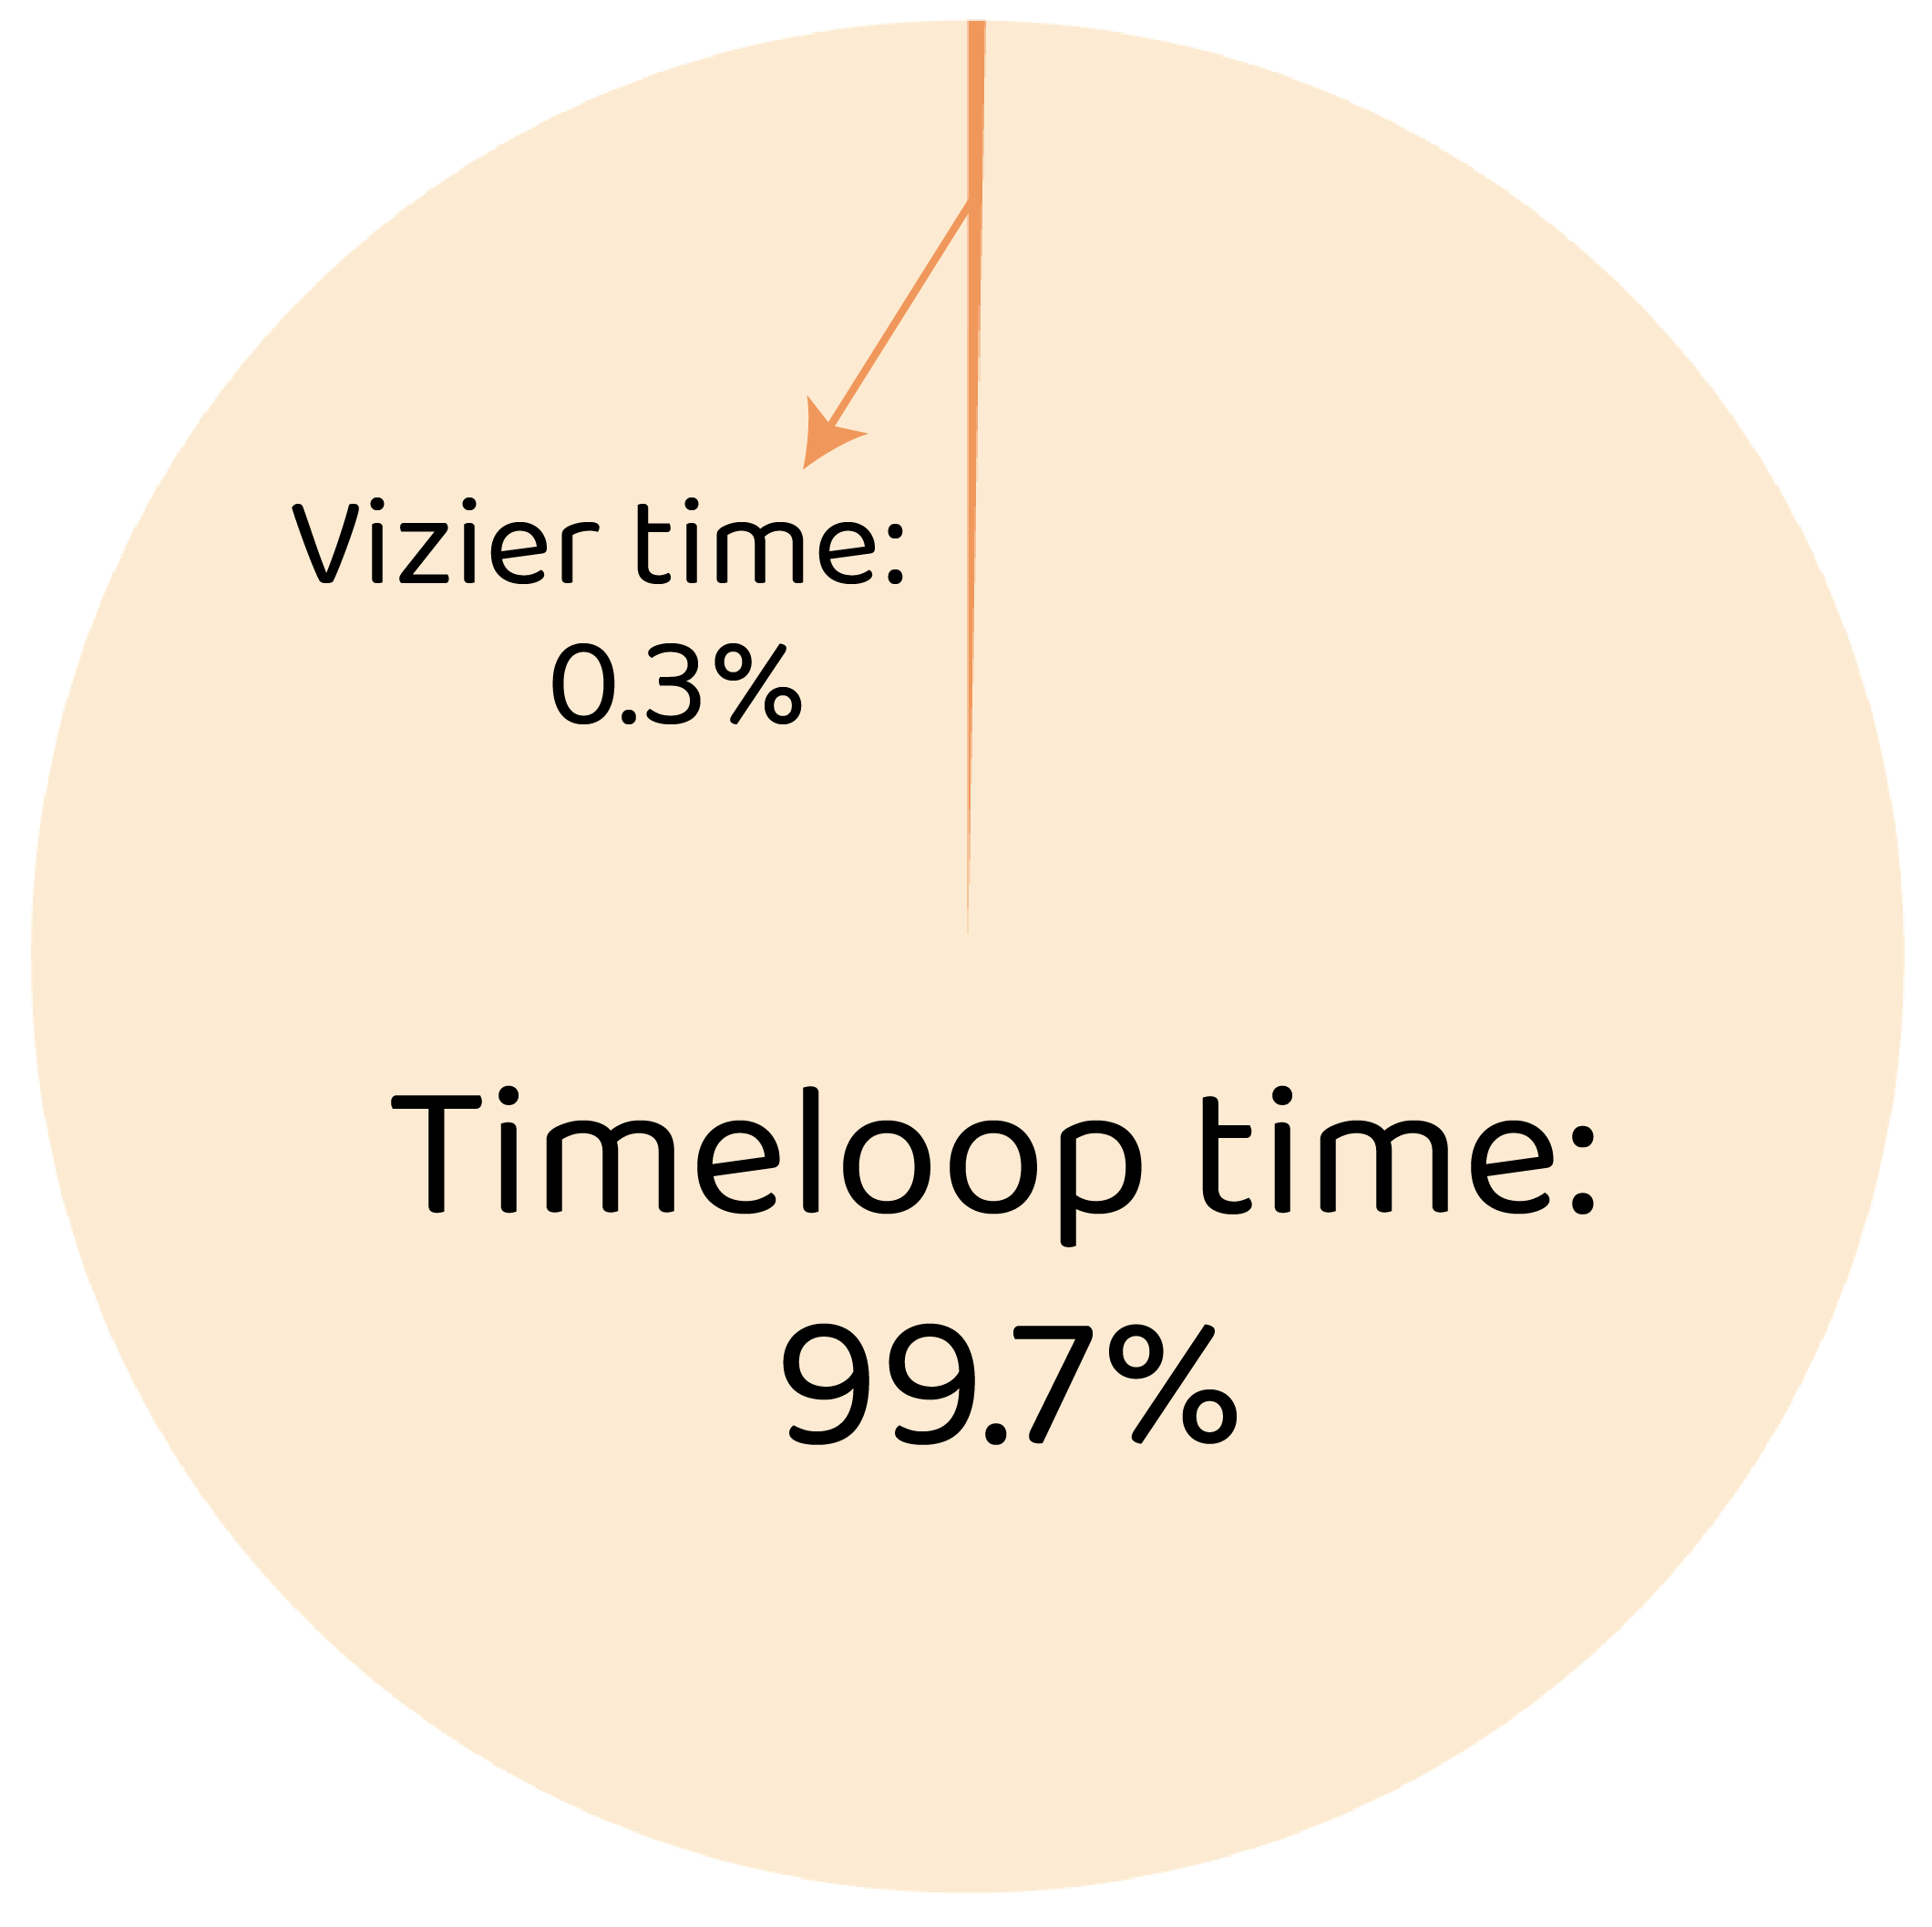
\includegraphics[width=\linewidth]{fig3/timeloop_vs_vizier.png}
% % %     \caption{Per-trial wall-clock breakdown.}
% % %     \label{fig:timeloop-time}
% % %     \vspace{-10pt}
% % % \end{wrapfigure}
% % % Despite V0's improvements, it inherits the sequential dependence on external tiling tools (e.g., Timeloop) because it lacks a linear expression for non-linear tiling-fusion interactions. As shown in Figure~\ref{fig:timeloop-time}, Timeloop accounts for over 99\% of per-trial latency, creating a prohibitive bottleneck for multi-thousand-trial searches. To resolve this, CHEETAH-V1 internalizes tiling by precomputing Pareto-pruned configurations and encoding them as decision variables. This removes Timeloop from the critical path, collapsing each trial to a single Vizier-proposal and LP-solve step. We start with introducing the preprocessing stage below before presenting the full formulation in Section~\ref{sec::v1}.

% % % % The limitations of prior work is still inherited in the V0 formulation due to the difficulty of expressing non-linear relationships as linear constraints. Therefore tiling decisions $(\Tmax_i, \Tmin_i, t_i^k)$ are fixed constants provided by additional software, such as Timeloop. A natural question is whether this sequential dependence also creates a \emph{runtime} bottleneck. Figure~\ref{fig:timeloop-time} confirms that it does: across different models, Timeloop scheduling on average accounts for over 99\% of per-trial wall-clock time, while the Vizier proposal and fusion ILP together consume less than 1\% on average. Because the outer loop requires thousands of trials to converge, the cumulative cost of repeated Timeloop invocations dominates the total search budget. This observation motivates a key design choice in CHEETAH-V1: rather than calling Timeloop online during each trial, we precompute a Pareto-pruned set of tiling configurations once (Section~\ref{sec:pareto}) and encode the tiling selection as decision variables \emph{inside} the LP. This eliminates Timeloop from the per-trial critical path entirely, reducing each trial to a single Vizier-proposal$\,\to\,$LP-solve step.

% % % % CHEETAH-V1 captures tiling as a \emph{decision variable} inside the LP, enabling the solver to jointly optimize tiling and fusion. We start with describing our preprocessing stage in Section~\ref{sec:pareto} before presenting the full formulation in Section~\ref{sec::v1}.


% % % \paragraph{Pareto Pruning Pre-Pass} The raw tiling search space for a $7$-dimensional convolution loop with $3$ memory levels is $\mathcal O(10^7)$ configurations per operation. We reduce this to a tractable Pareto-optimal subset $\mathcal{C}_i$ for each operation $i$ via a pre-pass for (1) L1 feasibility where configurations whose tiled working set exceeds L1 scratchpad capacity $C_{L1}$ are discarded; (2) Pareto optimality where a configuration $c$ is retained only if no other configuration achieves both lower $\Tmax_i(c)$ \emph{and} smaller working-set size in the Global Buffer.

% % % In practice, Pareto pruning reduces $\mathcal O(10^7)$ raw configurations to $|\mathcal{C}_i| \approx 10^2$ to $10^3$ per operation. Timeloop is run once per (operation, configuration) pair, producing the triple $(\Tmin_i(c), \Tmax_i(c), t_i^k(c))$ for each retained configuration $c \in \mathcal{C}_i$. These are precomputed constants---the LP solver makes no Timeloop calls at solve time.

% % % \paragraph{Time-invariant Pareto fronts.}
% % % A key observation is that the Pareto front shape is invariant to memory time: configurations are ranked by compute cycles and working-set bytes, neither of which depends on bandwidth. Changing bandwidth rescales the DRAM access cost $t_i^k(c)$ uniformly. This means the Pareto-pruned configuration sets can be precomputed \emph{once} and reused across all Vizier trials that share the same compute configuration class, amortizing the expensive Timeloop precomputation.

% % % \subsubsection{The Joint CHEETAH-V1 LP Formulation}\label{sec::v1}

% % % \paragraph{From fixed constants to decision variables.}
% % % In static and V0 formulations, Timeloop selects a single tiling per operation externally and passes the results to the LP as fixed constants $\Tmax_i$, $\Tmin_i$, $t_i^k$. The DRAM savings from pinning tensor $k$ of operation $i$ is then simply $t_i^k \cdot p_{i,o(i)}^k$---a constant times a variable, which is already linear. V1 brings this tiling choice \emph{inside} the LP by introducing \textbf{tiling selection variables} $y_{i,c} \in [0,1]$, one per Pareto-optimal configuration $c \in \mathcal{C}_i$ from the pre-pass, with the constraint $\sum_c y_{i,c} = 1$ (exactly one configuration is selected per operation). The Timeloop-precomputed constants $\Tmax_i(c)$, $\Tmin_i(c)$, $t_i^k(c)$ now become \emph{per-configuration coefficients} indexed by $c$. This means the DRAM savings term becomes $t_i^k(c) \cdot y_{i,c} \cdot p_{\text{assoc}(i,k),\, o(i)}$. This is a product of \emph{two} decision variables, which is bilinear and cannot be handled by a convex programming directly.
 
% % % % \paragraph{Linearization via McCormick envelopes.}
% % % % We linearize this product exactly via the classical McCormick substitution. Specifically,  we introduce \textbf{auxiliary variables} $w_{i,c,k} := y_{i,c} \cdot p_{\text{assoc}(i,k),\, o(i)}$ that represent the joint effect of selecting tiling $c$ \emph{and} pinning tensor $k$, constrained by:
% % % % \begin{equation}
% % % % \label{eq:mccormick}
% % % % \begin{aligned}
% % % %     w_{i,c,k} &\leq y_{i,c}, \qquad
% % % %     w_{i,c,k} \leq p_{\text{assoc}(i,k),\, o(i)} \\
% % % %     w_{i,c,k} &\geq y_{i,c} + p_{\text{assoc}(i,k),\, o(i)} - 1, \qquad
% % % %     w_{i,c,k} \geq 0
% % % % \end{aligned}
% % % % \end{equation}
% % % % Since both factors lie in $[0,1]$, these four constraints force $w_{i,c,k} = y_{i,c} \cdot p$ at any integer vertex, requiring no manually tuned constants. Together, $y_{i,c}$ and $w_{i,c,k}$ account for 1.6M of the 2.08M variables in the \Vone~ LP (Table~\ref{tab:v1_scale}). \todo{change to MoE?}

% % % \paragraph{Linearization via McCormick envelopes.}
% % % We linearize this product exactly via the classical McCormick substitution \citep{mccormick1976computability}. Specifically, we introduce \textbf{auxiliary variables} $w_{i,c,k} := y_{i,c} \cdot p_{\text{assoc}(i,k),\, o(i)}$ that represent the joint effect of selecting tiling $c$ \emph{and} pinning tensor $k$, constrained by:
% % % \begin{equation}
% % % \label{eq:mccormick}
% % % \begin{aligned}
% % %     w_{i,c,k} &\leq y_{i,c}, \qquad
% % %     w_{i,c,k} \leq p_{\text{assoc}(i,k),\, o(i)} \\
% % %     w_{i,c,k} &\geq y_{i,c} + p_{\text{assoc}(i,k),\, o(i)} - 1, \qquad
% % %     w_{i,c,k} \geq 0
% % % \end{aligned}
% % % \end{equation}
% % % Since both factors lie in $[0,1]$, these four constraints force $w_{i,c,k} = y_{i,c} \cdot p$ at any integer vertex, requiring no manually tuned constants. Together, $y_{i,c}$ and $w_{i,c,k}$ constitute the majority of V1's decision variables (Table~\ref{tab:v1_scale}).
 

% % % % \paragraph{Full formulation.}
% % % % Combining tiling selection, time-indexed placement, rematerialization, and McCormick linearization, the full V1  formulation is:

% % % % \begin{equation}
% % % % % \label{eq:v1}
% % % % \begin{aligned}
% % % % \min \quad & \sum_{i \in \mathcal{N}} T_i + \sum_{i \in \mathcal{N}} \sum_{t \in \mathcal{T}} c_i^{\text{remat}} \, r_{i,t} \\[4pt]
% % % % \text{s.t.} \quad
% % % % & \sum_{c \in \mathcal{C}_i} y_{i,c} = 1 & \forall\, i \in \mathcal{N} \\[3pt]
% % % % & T_i \geq \sum_{c \in \mathcal{C}_i} \Tmax_i(c)\, y_{i,c} - \sum_{c \in \mathcal{C}_i} \sum_{k} t_i^k(c)\, w_{i,c,k} & \forall\, i \in \mathcal{N} \\[3pt]
% % % % & T_i \geq \sum_{c \in \mathcal{C}_i} \Tmin_i(c)\, y_{i,c} & \forall\, i \in \mathcal{N} \\[3pt]
% % % % & w_{i,c,k} \leq y_{i,c} & \forall\, i, c, k \\
% % % % & w_{i,c,k} \leq p_{\text{assoc}(i,k),\, o(i)} & \forall\, i, c, k \\
% % % % & w_{i,c,k} \geq y_{i,c} + p_{\text{assoc}(i,k),\, o(i)} - 1 & \forall\, i, c, k \\[3pt]
% % % % & \sum_{e \in \mathcal{E}} d_e\, p_{e,t} + \sum_{i \in \mathcal{N}} d_i^W\, p_{i,t}^W \leq \CGM & \forall\, t \in \mathcal{T} \\[3pt]
% % % % & p_{e,t} \leq p_{e,t-1} + r_{\text{src}(e),\, t} & \forall\, e, t > o(\text{src}(e)) \\
% % % % & p_{i,t}^W \leq p_{i,t-1}^W & \forall\, i, t > o(i) \\[3pt]
% % % % & r_{i,t} = 0 & \forall\, i, t \leq o(i) \\
% % % % & r_{i,t} \leq p_{e,t} & \forall\, e \in \text{in}(i), t > o(i) \\
% % % % & r_{i,t} \leq p_{i,t}^W & \forall\, i, t > o(i) \\[3pt]
% % % % & T_i, p_{e,t}, p_{i,t}^W, r_{i,t}, w_{i,c,k} \geq 0 &
% % % % \end{aligned}
% % % % \tag{\textcolor{skyblue}{V1}}\label{eq:v1}
% % % % \end{equation}
% % % % full formulation below in appendix 
% % % % \begin{equation}
% % % % \begin{aligned}
% % % % \min \quad & \sum_{i \in \mathcal{N}} T_i + \sum_{i \in \mathcal{N}} \sum_{t \in \mathcal{T}} c_i^{\text{remat}} \, r_{i,t} \\[4pt]
% % % % \text{s.t.} \quad
% % % % & \sum_{c \in \mathcal{C}_i} y_{i,c} = 1 & \forall\, i \in \mathcal{N} \\[3pt]
% % % % & T_i \geq \max\!\left(\sum_{c \in \mathcal{C}_i} \Tmin_i(c)\, y_{i,c},\;\; \sum_{c \in \mathcal{C}_i} \Tmax_i(c)\, y_{i,c} - \sum_{c \in \mathcal{C}_i} \sum_{k} t_i^k(c)\, w_{i,c,k}\right) & \forall\, i \in \mathcal{N} \\[3pt]
% % % % & w_{i,c,k} \leq y_{i,c}, \quad w_{i,c,k} \leq p_{\text{assoc}(i,k),\, o(i)}, \quad w_{i,c,k} \geq y_{i,c} + p_{\text{assoc}(i,k),\, o(i)} - 1 & \forall\, i, c, k \\[3pt]
% % % % & \sum_{e \in \mathcal{E}} d_e\, p_{e,t} + \sum_{i \in \mathcal{N}} d_i^W\, p_{i,t}^W \leq \CGM & \forall\, t \in \mathcal{T} \\[3pt]
% % % % & p_{e,t} \leq p_{e,t-1} + r_{\text{src}(e),\, t} & \forall\, e,\, t > o(\text{src}(e)) \\
% % % % & p_{i,t}^W \leq p_{i,t-1}^W & \forall\, i,\, t > o(i) \\[3pt]
% % % % & r_{i,t} = 0 \;\; \forall\, t \leq o(i); \quad r_{i,t} \leq \min\!\big(p_{e,t},\, p_{i,t}^W\big) \;\; \forall\, e \in \text{in}(i),\, t > o(i) \\[3pt]
% % % % & T_i,\, p_{e,t},\, p_{i,t}^W,\, r_{i,t},\, w_{i,c,k} \geq 0 &
% % % % \end{aligned}
% % % % \tag{\textcolor{skyblue}{V1}}\label{eq:v1}
% % % % \end{equation}

% % % \paragraph{Variable and constraint digest.}
% % % The V1 formulation inherits all the features of the V0 formulation, and additionally captures tiling by introducing selection variables
% % % $y_{i,c} \in [0,1]$, constrained by $\sum_c y_{i,c} = 1$, to choose
% % % from $|\mathcal{C}_i|$ Pareto-optimal configurations.
% % % Each configuration defines compute costs $T_i^{\max}(c)$,
% % % $T_i^{\min}(c)$, and per-tensor DRAM savings $t_i^k(c)$.
% % % We linearize the resulting bilinear DRAM-savings term exactly via
% % % McCormick auxiliary variables $w_{i,c,k}$, which enforce $w_{i,c,k} \;=\; y_{i,c} \cdot p_{\mathrm{assoc}(i,k),\,o(i)}$ at integer vertices without a relaxation gap.

% % % Per-operation latency $T_i$ is lower-bounded by the weighted
% % % configuration floor $\sum_c T_i^{\min}(c)\, y_{i,c}$ and the weighted
% % % off-chip cost $\sum_c T_i^{\max}(c)\, y_{i,c}$ minus achievable savings
% % % $\sum_{c,k} t_i^k(c)\, w_{i,c,k}$.
% % % This coupling enables the solver to accept sub-optimal local tiling
% % % (higher $T_i^{\max}$) if its smaller memory footprint unlocks global
% % % fusion gains that outweigh the compute-utilization loss.
% % % Capacity and persistence constraints carry over from V0, utilizing
% % % edge-indexed placement $p_{e,t}$ to handle multi-fanout nodes.
% % % For DeepSeek-V3, the V1 LP scales to approximately $2{,}504{,}019$ variables, $2{,}983{,}450$ constraints, and $6{,}094{,}156$ non-zeros. Table~\ref{tab:v1_scale} provides a representative breakdown, Table~\ref{tab:comparison} summarizes features of each more powerful formulation; full per-model sizes are in Table~\ref{tab:exp1_lp_sizes} and \ref{tab:exp2_cluster_lp_sizes}. 



% % % % The V1 formulation extends V0 by making the tiling configuration a decision variable. The selection variables $y_{i,c} \in [0,1]$, with $\sum_c y_{i,c} = 1$, choose among $|\mathcal{C}_i|$ Pareto-optimal tiling configurations precomputed by Timeloop (Section~\ref{sec:pareto}). Each configuration $c$ determines the operation's compute cost $T_i^{\max}(c)$, on-chip floor $T_i^{\min}(c)$, and per-tensor DRAM savings $t_i^k(c)$.
% % % % The DRAM savings term $t_i^k(c) \cdot y_{i,c} \cdot p_{\text{assoc}(i,k),\,o(i)}$ 
% % % % is bilinear in the tiling selection and placement variables; we linearize it 
% % % % via McCormick auxiliary variables $w_{i,c,k}$, constrained by 
% % % % $w_{i,c,k} \leq y_{i,c}$, $w_{i,c,k} \leq p_{\text{assoc}(i,k),\,o(i)}$, and 
% % % % $w_{i,c,k} \geq y_{i,c} + p_{\text{assoc}(i,k),\,o(i)} - 1$. 
% % % % These three inequalities force $w_{i,c,k} = y_{i,c} \cdot p_{\text{assoc}(i,k),\,o(i)}$ 
% % % % at any integer-feasible point (\cref{prop:mccormick_exact}), so the LP exactly captures the 
% % % % bilinear interaction without introducing any relaxation gap at integer vertices.
% % % % The $T_i$ lower bound now takes the maximum of two configuration-dependent terms: the weighted on-chip floor $\sum_c T_i^{\min}(c)\, y_{i,c}$ and the weighted off-chip cost minus achievable savings $\sum_c T_i^{\max}(c)\, y_{i,c} - \sum_{c,k} t_i^k(c)\, w_{i,c,k}$.
% % % % This coupling is the core novelty of V1: the solver can accept a tiling with higher $T_i^{\max}(c)$ (lower compute utilization) if its smaller working set enables pinning decisions that reduce total DRAM traffic by more than the utilization loss.
% % % % All remaining constraints---memory capacity, persistence, and rematerialization---carry over from V0 with edge-indexed placement variables $p_{e,t}$ replacing per-tensor $p_{i,t}^k$ to correctly handle skip connections and multi-fanout nodes. For our largest workload, DeepSeek-V3 ($L \approx 6{,}300$ operations), the V1 LP contains approximately 2.5M variables, 3.0M constraints, and 6.1M nonzeros. Table~\ref{tab:v1_scale} provides a representative breakdown; full per-model sizes are in Table~\ref{tab:v1_scale}. 
% % % % \paragraph{Key constraint interactions.}
% % % % The execution-time constraints (lines 2--3: the upper and lower bounds for $T_i$) capture the central trade-off that is unique to \Vone: the LP must commit to a tiling configuration $c$ (via $y_{i,c}$) that sets both the baseline compute cost $\Tmax_i(c)$ and the achievable DRAM savings $t_i^k(c)$. A configuration with smaller tiles may have higher $\Tmax_i(c)$ (lower compute utilization) but smaller working sets, enabling more aggressive pinning. The LP balances these trade-offs simultaneously---precisely the cross-stage interaction that the sequential pipeline cannot discover.
 
% % % % The edge-indexed persistence constraint (line 8: $p_{e,t} \leq p_{e,t-1} + r_{\text{src}(e),\, t}$) and the memory capacity constraint (line 7: lower bound on $\CGM$) are inherited from \Vzero, which introduced per-edge placement variables $p_{e,t}$ to correctly model skip connections. \Vone~ extends this by coupling edge sizes to the tiling selection---since different configurations $c$ produce different activation working sets, the LP can now jointly reason about how tiling choices affect memory pressure across skip connections.


% % % \begin{figure}[ht!]
% % % \begin{minipage}[t]{0.48\textwidth}
% % % \vspace{0pt}
% % % \centering
% % % \captionof{table}{V1 variable and constraint counts
% % % (representative, DeepSeek-V3).}
% % % \label{tab:v1_scale}
% % % \footnotesize
% % % \begin{tabular}{@{}ll@{}}
% % % \toprule
% % % \textbf{Variable} & \textbf{Role} \\
% % % \midrule
% % % $T_i$       & Per-operation execution time \\
% % % $y_{i,c}$   & Tiling config selection ($|\mathcal{C}_i|$ options) \\
% % % $p_{e,t}$   & Edge-indexed activation placement \\
% % % $p_{i,t}^W$ & Weight placement \\
% % % $r_{i,t}$   & Rematerialization indicator \\
% % % $w_{i,c,k}$ & McCormick auxiliaries ($y_{i,c} \cdot p$) \\
% % % % \midrule
% % % % \multicolumn{2}{@{}l}{\textbf{DeepSeek-V3 totals}
% % % %                        ($L \approx 6{,}300$)} \\
% % % % \midrule
% % % % Variables   & $2{,}504{,}019$ \\
% % % % Constraints & $2{,}983{,}450$ \\
% % % % Nonzeros    & $6{,}094{,}156$ \\
% % % \bottomrule
% % % \end{tabular}
% % % \end{minipage}%
% % % \hspace{0.02\textwidth}%
% % % \begin{minipage}[t]{0.48\textwidth}
% % % \vspace{0pt}
% % % \centering
% % % \captionof{table}{Comparison of static, V0, and V1 formulations.}
% % % \label{tab:comparison}
% % % \footnotesize
% % % \begin{tabular}{@{}lccc@{}}
% % % \toprule
% % % \textbf{Property} & \textbf{Static} & \textbf{V0} & \textbf{V1} \\
% % % \midrule
% % % Joint tiling + fusion    & $\times$ & $\times$   & \checkmark \\
% % % Time-indexed placement   & $\times$ & \checkmark & \checkmark \\
% % % Rematerialization        & $\times$ & \checkmark & \checkmark \\
% % % Relaxed skip connections & $\times$ & Partial    & \checkmark \\
% % % \bottomrule
% % % \end{tabular}

% % % \medskip
% % % \raggedright
% % % \footnotesize
% % % % \textbf{Comparison across formulations.}
% % % % Table~\ref{tab:comparison} summarizes the progression from the
% % % % static formulation through V0 to V1.
% % % \end{minipage}
% % % \end{figure}


% % % % \begin{table}[ht!]
% % % % \centering
% % % % \caption{V1 variable and constraint counts (representative, DeepSeek-V3).}
% % % % \label{tab:v1_scale}
% % % % \small
% % % % \begin{tabular}{lrl}
% % % % \toprule
% % % % \textbf{Variable} & \textbf{Role} \\
% % % % \midrule
% % % % $T_i$ & Per-operation execution time \\
% % % % $y_{i,c}$ & Tiling configuration selection ($|\mathcal{C}_i|$ options per op) \\
% % % % $p_{e,t}$ & Edge-indexed activation placement \\
% % % % $p_{i,t}^W$ & Weight placement \\
% % % % $r_{i,t}$ & Rematerialization indicator \\
% % % % $w_{i,c,k}$ & McCormick auxiliaries ($y_{i,c} \cdot p$) \\
% % % % \midrule
% % % % \multicolumn{2}{l}{\textbf{DeepSeek-V3 totals} ($L \approx 6{,}300$)} \\
% % % % \midrule
% % % % Variables & 2,504,019 \\
% % % % Constraints & 2,983,450 \\
% % % % Nonzeros & 6,094,156 \\
% % % % \bottomrule
% % % % \end{tabular}
% % % % \end{table}
% % % % \paragraph{Comparison across formulations.}
% % % % Table~\ref{tab:comparison} summarizes the progression from static through V0 to V1.
% % % % \begin{table}[ht!]
% % % % \centering
% % % % \caption{Comparison of static, V0, and V1 formulations.}
% % % % \label{tab:comparison}
% % % % \small
% % % % \begin{tabular}{lccc}
% % % % \toprule
% % % % \textbf{Property} & \textbf{static} & \textbf{V0} & \textbf{V1} \\
% % % % \midrule
% % % % Joint tiling + fusion & \texttimes & \texttimes & \checkmark \\
% % % % Time-indexed placement & \texttimes & \checkmark & \checkmark \\
% % % % Rematerialization & \texttimes & \checkmark & \checkmark \\
% % % % Relaxed skip connections & \texttimes & Partial & \checkmark \\
% % % % % Config-dependent DRAM savings & \texttimes & \texttimes & \checkmark \\ 
% % % % % Bilinear linearization & --- & --- & McCormick \\
% % % % \bottomrule
% % % % \end{tabular}
% % % % \end{table}

% % % % \paragraph{Structural invariance for efficient LLM integration.}
% % % % A practical advantage of both our LP formulations is that the constraint matrix sparsity pattern is invariant across hardware configurations---only the numerical coefficients change. This means:
% % % % \begin{itemize}
% % % %     \item The LP solver's preconditioner can be designed once per neural network model and reused across all Vizier trials.
% % % %     \item An LLM-Architect can reason about constraint structure (which constraints are binding, which variables are fractional) without needing to understand the full LP.
% % % %     \item Warm-starting from a previous trial's LP solution is straightforward since the variable indexing is stable.
% % % % \end{itemize}

% % % \subsection{Strategic Intelligence: LLM-Guided Outer Search}
% % % \label{sec:llm_outer}
% % % We use Google Vizier as a black-box Bayesian optimizer to propose hardware configurations. While effective, vanilla Vizier treats search as pure function optimization, often requiring thousands of iterations to identify suboptimal regions without leveraging structural hardware-workload knowledge. To address this, we introduce an LLM-guided outer-loop controller based on SkyDiscovery that reasons about co-design decisions. By learning from a causal ledger of past trials and Lagrangian dual signals from the LP solver, the LLM proposes meaningful, constrained search-space candidates. This integration is enabled by the CHEETAH-V1 formulation, which removes the Timeloop bottleneck to reduce trial times from days to hours.The LLM-Architect reduces wasted trials by intelligently steering Vizier’s search without altering the inner solver or its optimality certificates. In this hybrid loop, the LLM determines global architectural regions, Vizier performs local Bayesian optimization within those patches, and the large-scale V1 LP solver evaluates each concrete candidate. The LLM-Architect loop proceeds as follows: 
% % % % We use Vizier as a black-box Bayesian optimizer to propose candidate hardware configurations. While effective, Vizier search strategies (LCS, UCB, etc) requires thousands of iterations explore and learn which regions are suboptimal and treats the search as a pure function optimization problem without leveraging structural knowledge about hardware-workload interactions.
% % % % We leverage an LLM-guided outer-loop controller that learns from logs of thousands of past co-design trials to propose meaningful search-space candidates for Vizier. This is a SkyDiscovery based outer LLM layer which reasons about hardware-software co-design decisions and learns from a causal ledger of constantly updated logs across trials, as well as feed-back signal such as dual variables through the LP solve. This is possible for CHEETAH-V1 LP formulation, since it removes the Timeloop-in-the-loop constraint, thus reducing the co-design problem from days to hours, and permitting the LLM outer loop. 

% % % % The LLM-Architect does not change the inner solver, and retains all the optimal certificates of the V1 LP formulation, but intelligently changes where the Vizier outer hardware optimizer searches to reduce wasted trials. The LLM proposes global decisions to determine constrained regions of the hardware search space; Vizier then performs local Bayesian optimization inside those regions; which then passes downstream into a large scale LP solver for the V1 formulation to evaluate each concrete candidate. The LLM-Architect loop proceeds as follows:

% % % \begin{enumerate}[leftmargin=1.6em, itemsep=4pt]

% % % \item \textbf{Extraction.}
% % % Deterministic scripts summarize recent trials into a \emph{Causal
% % % Ledger}. Each record includes hardware parameters, validity, Perf/TDP,
% % % LP cycles, capacity duals/slacks, bandwidth sensitivity, MFU, memory
% % % utilization, roofline gap, failure class, and LP solver metrics.

% % % \item \textbf{Context building.}
% % % The last $N$ trials and the Causal Ledger are compressed into a compact
% % % JSON context for the Architect. The context emphasizes empirical
% % % feasibility, observed invalid regions, best known valid designs, and
% % % physical audit signals.

% % % \item \textbf{Architect.}
% % % The online Architect, implemented as Qwen2.5-7B-Instruct with a LoRA
% % % adapter trained on past trial logs, diagnoses the dominant bottleneck
% % % and emits a campaign patch. The patch constrains macro-architectural
% % % search decisions such as Global Memory, DRAM bandwidth, total MACs,
% % % systolic shape, PE grid, and batch size. A larger teacher model,
% % % DeepSeek-V3.2, was used offline to generate or critique campaign labels
% % % but is not in the live loop.

% % % \item \textbf{Campaign validation.}
% % % A deterministic validator clips or rejects the LLM patch to enforce
% % % legal hardware ranges, TDP and area limits, MAC caps, CGM feasibility
% % % floors, compute/bandwidth coupling, and roofline constraints. This
% % % prevents the LLM from proposing physically implausible regions such as
% % % maximum-MAC/minimum-bandwidth designs.

% % % \item \textbf{Local optimization.}
% % % Vizier is initialized inside the validated patch and warm-started with
% % % prior trials that lie in the same region. Vizier then samples concrete
% % % hardware candidates within the approved campaign. The LLM therefore
% % % chooses the high-level architectural neighbourhood, while Vizier
% % % performs local adaptive optimization.

% % % \item \textbf{Unified V1 evaluation.}
% % % The large-scale LP solver evaluates each candidate by solving the V1
% % % joint tiling-fusion-placement LP using saved Pareto $\mathcal{C}$-sets.
% % % It returns the objective, cycles, selected tiling configurations,
% % % placement/rematerialization decisions, dual/slack summaries, and
% % % solver-quality diagnostics.

% % % \item \textbf{Roofline audit.}
% % % A deterministic Roofline Auditor checks whether the predicted latency
% % % is physically plausible. For each candidate we compute
% % % \begin{align}
% % %     t_{\text{compute}} &=
% % %         \frac{\text{useful FLOPs}}{\text{peak FLOPs/s}},
% % %     \qquad
% % %     t_{\text{memory}}  =
% % %         \frac{\text{post-placement DRAM bytes}}{\text{peak bandwidth}},
% % %     \nonumber\\
% % %     t_{\text{ideal}}   &=
% % %         \max\!\left(t_{\text{compute}},\, t_{\text{memory}}\right).
% % %     \label{eq:roofline_audit}
% % % \end{align}
% % % A candidate is rejected if the solver-reported latency falls below this
% % % lower bound, or if MFU or memory utilization exceeds 1.0 within
% % % tolerance.

% % % \item \textbf{Ledger update.}
% % % The loop records the campaign hypothesis, intervention, observed
% % % invalid-rate change, MFU change, roofline validity, and best Perf/TDP
% % % change. The ledger also records forbidden regions when a campaign
% % % produces excessive invalid trials.

% % % \end{enumerate}

% % % \noindent The Architect receives workload summaries, invalid-rate
% % % history, MFU, roofline signals, prior valid regions, normalized LP duals,
% % % and bandwidth sensitivities. The system starts from a safe empirically
% % % valid patch and permits duals only to make bounded edits, such as raising
% % % the CGM floor, increasing bandwidth, reducing MAC count, or changing
% % % systolic shapes. The validator rejects any dual-guided patch that
% % % excludes known high-performing valid regions or predicts a substantially
% % % worse feasible rate. This provides controlled architectural feedback in
% % % addition to prompt input.


% % % % \todo{Expand this section once the LLM+RL experimental protocol is finalized. Key questions to address: (1) Which LLM is used and how is it prompted? (2) How are LLM proposals integrated with Vizier's Bayesian model? (3) What is the sample efficiency improvement over pure Vizier?}





% % % edit for page limit 

% % \section{Methodology}
% % \label{sec:methods}

% % We present the CHEETAH (\acroletter{C}o-designed \acroletter{H}ardware \acroletter{E}xploration via \acroletter{E}fficient \acroletter{T}hroughput and \acroletter{H}ybrid-search) framework in three parts: Section~\ref{sec:v0} introduces CHEETAH-V0, which extends the static fusion ILP with time-indexed placement and rematerialization. Section~\ref{sec:v1} presents CHEETAH-V1, which jointly optimizes tiling and fusion via McCormick linearization. Section~\ref{sec:llm_outer} describes the LLM-Architect outer loop.


% % % \subsection{\Vzero~: Multi-Period Placement with Rematerialization}
% % \subsection{CHEETAH-V0: Multi-Period Placement with Rematerialization}
% % \label{sec:v0}

% % Our first extension models the neural network's execution as a sequence of $T$ discrete timesteps (one per operation in execution order). This decides at which time, which tensor is pinned, evicted, or recomputed to optimally minimize cycle counts. The key features are:

% % \paragraph{Time-indexed placement.}
% % Instead of a single binary $p_i^k$ per tensor, we introduce $p_{i,t}^k \in [0,1]$ for each tensor $k$ of layer $i$ at each timestep $t$. A tensor can be pinned at timestep $t=5$, and evicted at $t=10$. This models a dynamic memory manager within a single inference pass.

% % \paragraph{Rematerialization.}
% % Rather than always paying DRAM bandwidth to reload an evicted tensor, we introduce variables $r_{i,t} \in [0,1]$ indicating that layer $i$ is recomputed at timestep $t$ to restore its output to the Global Buffer. This is particularly valuable for models such as EfficientNet, where depthwise convolutions account for only ${\sim}5\%$ of total FLOPs but produce large activation tensors. Recomputing a depthwise layer to avoid re-reading 6\,MiB from DRAM at 256\,GB/s can be faster than the DRAM reload itself.

% % \paragraph{Relaxed skip-connection handling.}
% % We lift the limitation of our baseline original ILP, which restricts activation pinning to consecutively-executed operations and limits multi-fanout nodes so that at most one consumer benefits from on-chip data. CHEETAH-V0 uses edge-indexed placement variables $p_{e,t}$ for each edge $e \in \mathcal{E}$ of the dataflow graph, correctly modeling the case where one consumer of a skip connection benefits from on-chip data while another does not.

% % The CHEETAH-V0 LP formulation is:
% % \begin{equation}
% % % \label{eq:v0}
% % \begin{aligned}
% % \min \quad & \sum_{i \in \mathcal{N}} T_i + \sum_{i \in \mathcal{N}} \sum_{t \in \mathcal{T}} c_i^{\text{remat}} \, r_{i,t} \\
% % \text{s.t.} \quad
% % & T_i \geq \Tmax_i - \sum_{k \in \{I,O,W\}} t_i^k \cdot p_{i,o(i)}^k & \forall\, i \in \mathcal{N} \\
% % & T_i \geq \Tmin_i & \forall\, i \in \mathcal{N} \\
% % & \sum_{i \in \mathcal{N}} \sum_{k} d_i^k \, p_{i,t}^k \leq \CGM & \forall\, t \in \mathcal{T} \\
% % & p_{i,t}^k \leq p_{i,t-1}^k + r_{i,t} & \forall\, i, t, k \in \{I,O\} \\
% % & p_{i,t}^W \leq p_{i,t-1}^W & \forall\, i, t \\
% % & r_{i,t} = 0 & \forall\, i, t \leq o(i) \\
% % & 0 \leq p_{i,t}^k, r_{i,t} \leq 1 &
% % \end{aligned}
% % \tag{V0}\label{eq:v0}
% % \end{equation}


% % where $o(i)$ is the execution order of operation $i$, $d_i^k$ is the byte size of tensor $k$ for layer $i$, and $c_i^{\text{remat}}$ is the recomputation cost.

% % \paragraph{Variable and constraint digest.}
% % The V0 objective minimizes the sum of execution times $\sum_i T_i$ and
% % rematerialization costs $c_i^{\text{remat}}\, r_{i,t}$.
% % Per-operation latency $T_i$ is lower-bounded by the physical on-chip
% % floor $T_i^{\min}$ and the off-chip time $T_i^{\max}$ adjusted for DRAM
% % savings $t_i^k \cdot p_{i,o(i)}^k$ from pinned tensors.
% % Placement variables $p_{i,t}^k \in [0,1]$ track Global Memory residency
% % for inputs, outputs, and weights at each timestep, subject to a global
% % capacity constraint $C_{\text{GM}}$. Persistence is governed by $p_{i,t}^k \;\leq\; p_{i,t-1}^k + r_{i,t},$ enforcing that activations are either resident from the previous timestep
% % or recomputed; weight tensors satisfy the stricter monotone constraint
% % $p_{i,t}^W \leq p_{i,t-1}^W$, as weights cannot be rematerialized.
% % Rematerialization $r_{i,t}$ is only permitted post-execution
% % ($t > o(i)$) and requires on-chip availability of both inputs and
% % weights.
% % For DeepSeek-V3 ($L \approx 6{,}300$), this formulation yields a
% % large-scale program with approximately 3.3M variables and 3.7M
% % constraints.


% % % \subsection{\textcolor{skyblue}{V1}: Joint Tiling and Fusion via McCormick Linearization}
% % \subsection{CHEETAH-V1: Joint Tiling and Fusion via McCormick Linearization}
% % \label{sec:v1}

% % \begin{wrapfigure}{r}{0.2\linewidth}
% %     \vspace{-12pt}
% %     \centering
% %     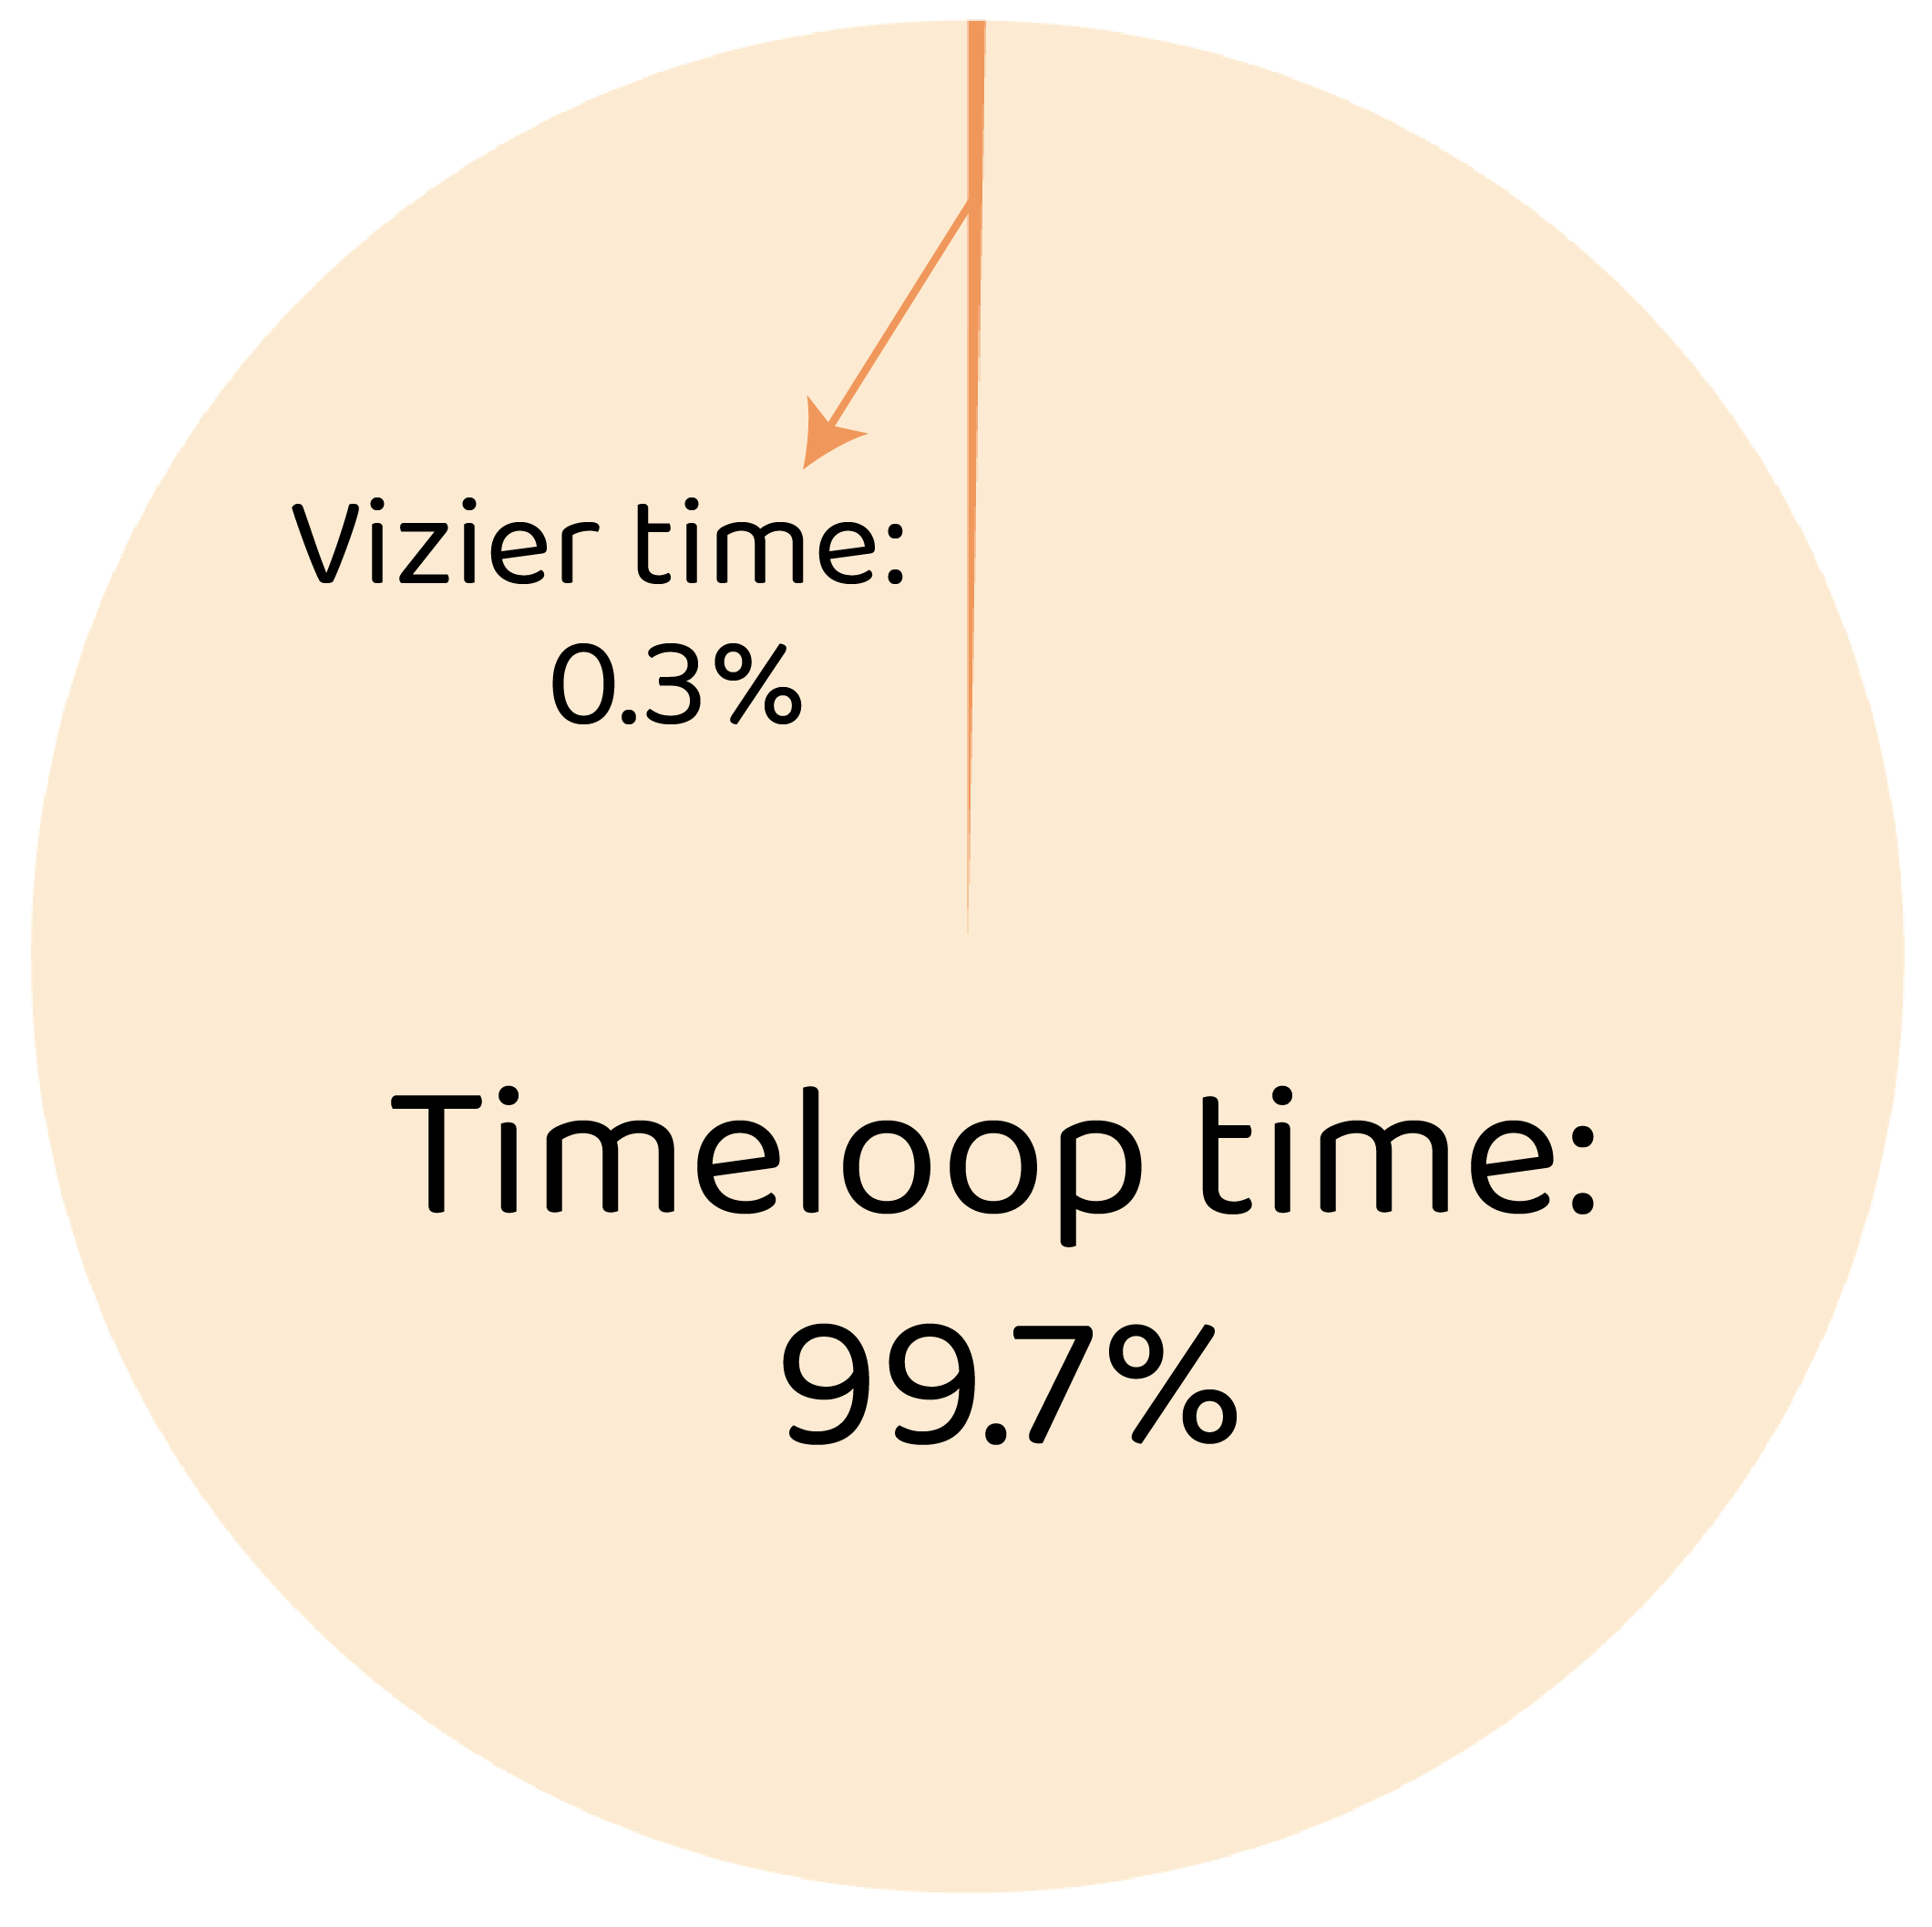
\includegraphics[width=\linewidth]{fig3/timeloop_vs_vizier.png}
% %     \caption{Per-trial wall-clock breakdown.}
% %     \label{fig:timeloop-time}
% %     \vspace{-10pt}
% % \end{wrapfigure}
% % Despite V0's improvements, it inherits the sequential dependence on external tiling tools (e.g., Timeloop) because it lacks a linear expression for non-linear tiling-fusion interactions. As shown in Figure~\ref{fig:timeloop-time}, Timeloop accounts for over 99\% of per-trial latency, creating a prohibitive bottleneck for multi-thousand-trial searches. To resolve this, CHEETAH-V1 internalizes tiling by precomputing Pareto-pruned configurations and encoding them as decision variables. This removes Timeloop from the critical path, collapsing each trial to a single Vizier-proposal and LP-solve step. We start with introducing the preprocessing stage below before presenting the full formulation in Section~\ref{sec::v1}.

% % % The limitations of prior work is still inherited in the V0 formulation due to the difficulty of expressing non-linear relationships as linear constraints. Therefore tiling decisions $(\Tmax_i, \Tmin_i, t_i^k)$ are fixed constants provided by additional software, such as Timeloop. A natural question is whether this sequential dependence also creates a \emph{runtime} bottleneck. Figure~\ref{fig:timeloop-time} confirms that it does: across different models, Timeloop scheduling on average accounts for over 99\% of per-trial wall-clock time, while the Vizier proposal and fusion ILP together consume less than 1\% on average. Because the outer loop requires thousands of trials to converge, the cumulative cost of repeated Timeloop invocations dominates the total search budget. This observation motivates a key design choice in CHEETAH-V1: rather than calling Timeloop online during each trial, we precompute a Pareto-pruned set of tiling configurations once (Section~\ref{sec:pareto}) and encode the tiling selection as decision variables \emph{inside} the LP. This eliminates Timeloop from the per-trial critical path entirely, reducing each trial to a single Vizier-proposal$\,\to\,$LP-solve step.

% % % CHEETAH-V1 captures tiling as a \emph{decision variable} inside the LP, enabling the solver to jointly optimize tiling and fusion. We start with describing our preprocessing stage in Section~\ref{sec:pareto} before presenting the full formulation in Section~\ref{sec::v1}.


% % \paragraph{Pareto Pruning Pre-Pass.} The raw tiling search space for a $7$-dimensional convolution loop with $3$ memory levels is $\mathcal O(10^7)$ configurations per operation. We reduce this to a tractable Pareto-optimal subset $\mathcal{C}_i$ for each operation $i$ via a pre-pass for (1) L1 feasibility where configurations whose tiled working set exceeds L1 scratchpad capacity $C_{L1}$ are discarded; (2) Pareto optimality where a configuration $c$ is retained only if no other configuration achieves both lower $\Tmax_i(c)$ \emph{and} smaller working-set size in the Global Buffer.

% % In practice, Pareto pruning reduces $\mathcal O(10^7)$ raw configurations to $|\mathcal{C}_i| \approx 10^2$ to $10^3$ per operation. Timeloop is run once per (operation, configuration) pair, producing the triple $(\Tmin_i(c), \Tmax_i(c), t_i^k(c))$ for each retained configuration $c \in \mathcal{C}_i$. These are precomputed constants---the LP solver makes no Timeloop calls at solve time.

% % \paragraph{Time-invariant Pareto fronts.}
% % A key observation is that the Pareto front shape is invariant to memory time: configurations are ranked by compute cycles and working-set bytes, neither of which depends on bandwidth. Changing bandwidth rescales the DRAM access cost $t_i^k(c)$ uniformly. This means the Pareto-pruned configuration sets can be precomputed \emph{once} and reused across all Vizier trials that share the same compute configuration class, amortizing the expensive Timeloop precomputation.

% % % \subsubsection{The Joint CHEETAH-V1 LP Formulation}\label{sec::v1}

% % \paragraph{From fixed constants to decision variables.}
% % In static and V0 formulations, Timeloop selects a single tiling per operation externally and passes the results to the LP as fixed constants $\Tmax_i$, $\Tmin_i$, $t_i^k$. The DRAM savings from pinning tensor $k$ of operation $i$ is then simply $t_i^k \cdot p_{i,o(i)}^k$---a constant times a variable, which is already linear. V1 brings this tiling choice \emph{inside} the LP by introducing \textbf{tiling selection variables} $y_{i,c} \in [0,1]$, one per Pareto-optimal configuration $c \in \mathcal{C}_i$ from the pre-pass, with the constraint $\sum_c y_{i,c} = 1$ (exactly one configuration is selected per operation). The Timeloop-precomputed constants $\Tmax_i(c)$, $\Tmin_i(c)$, $t_i^k(c)$ now become \emph{per-configuration coefficients} indexed by $c$. This means the DRAM savings term becomes $t_i^k(c) \cdot y_{i,c} \cdot p_{\text{assoc}(i,k),\, o(i)}$. This is a product of \emph{two} decision variables, which is bilinear and cannot be handled by a convex programming directly.
 
% % % \paragraph{Linearization via McCormick envelopes.}
% % % We linearize this product exactly via the classical McCormick substitution. Specifically,  we introduce \textbf{auxiliary variables} $w_{i,c,k} := y_{i,c} \cdot p_{\text{assoc}(i,k),\, o(i)}$ that represent the joint effect of selecting tiling $c$ \emph{and} pinning tensor $k$, constrained by:
% % % \begin{equation}
% % % \label{eq:mccormick}
% % % \begin{aligned}
% % %     w_{i,c,k} &\leq y_{i,c}, \qquad
% % %     w_{i,c,k} \leq p_{\text{assoc}(i,k),\, o(i)} \\
% % %     w_{i,c,k} &\geq y_{i,c} + p_{\text{assoc}(i,k),\, o(i)} - 1, \qquad
% % %     w_{i,c,k} \geq 0
% % % \end{aligned}
% % % \end{equation}
% % % Since both factors lie in $[0,1]$, these four constraints force $w_{i,c,k} = y_{i,c} \cdot p$ at any integer vertex, requiring no manually tuned constants. Together, $y_{i,c}$ and $w_{i,c,k}$ account for 1.6M of the 2.08M variables in the \Vone~ LP (Table~\ref{tab:v1_scale}). \todo{change to MoE?}

% % \paragraph{Linearization via McCormick envelopes.}
% % We linearize this product exactly via the classical McCormick substitution \citep{mccormick1976computability}. Specifically, we introduce \textbf{auxiliary variables} $w_{i,c,k} := y_{i,c} \cdot p_{\text{assoc}(i,k),\, o(i)}$ that represent the joint effect of selecting tiling $c$ \emph{and} pinning tensor $k$, constrained by:
% % \begin{equation}
% % \label{eq:mccormick}
% % \begin{aligned}
% %     w_{i,c,k} &\leq y_{i,c}, \qquad
% %     w_{i,c,k} \leq p_{\text{assoc}(i,k),\, o(i)} \\
% %     w_{i,c,k} &\geq y_{i,c} + p_{\text{assoc}(i,k),\, o(i)} - 1, \qquad
% %     w_{i,c,k} \geq 0
% % \end{aligned}
% % \end{equation}
% % Since both factors lie in $[0,1]$, these four constraints force $w_{i,c,k} = y_{i,c} \cdot p$ at any integer vertex, requiring no manually tuned constants. Together, $y_{i,c}$ and $w_{i,c,k}$ constitute the majority of V1's decision variables (Table~\ref{tab:v1_scale}).

% % \paragraph{The Joint CHEETAH-V1 LP Formulation.}
% % Combining tiling selection, time-indexed placement, rematerialization, and McCormick linearization, the full V1 formulation is:
% % \begin{equation}
% % \begin{aligned}
% % \min \quad & \sum_{i \in \mathcal{N}} T_i + \sum_{i \in \mathcal{N}} \sum_{t \in \mathcal{T}} c_i^{\text{remat}} \, r_{i,t} \\[4pt]
% % \text{s.t.} \quad
% % & \sum_{c \in \mathcal{C}_i} y_{i,c} = 1 & \forall\, i \in \mathcal{N} \\[3pt]
% % & T_i \geq \max\!\left(\sum_{c \in \mathcal{C}_i} \Tmin_i(c)\, y_{i,c},\;\; \sum_{c \in \mathcal{C}_i} \Tmax_i(c)\, y_{i,c} - \sum_{c \in \mathcal{C}_i} \sum_{k} t_i^k(c)\, w_{i,c,k}\right) & \forall\, i \in \mathcal{N} \\[3pt]
% % & w_{i,c,k} \leq y_{i,c}, \quad w_{i,c,k} \leq p_{\text{assoc}(i,k),\, o(i)}, \quad w_{i,c,k} \geq y_{i,c} + p_{\text{assoc}(i,k),\, o(i)} - 1 & \forall\, i, c, k \\[3pt]
% % & \sum_{e \in \mathcal{E}} d_e\, p_{e,t} + \sum_{i \in \mathcal{N}} d_i^W\, p_{i,t}^W \leq \CGM & \forall\, t \in \mathcal{T} \\[3pt]
% % & p_{e,t} \leq p_{e,t-1} + r_{\text{src}(e),\, t} & \forall\, e,\, t > o(\text{src}(e)) \\
% % & p_{i,t}^W \leq p_{i,t-1}^W & \forall\, i,\, t > o(i) \\[3pt]
% % & r_{i,t} = 0 \;\; \forall\, t \leq o(i); \quad r_{i,t} \leq \min\!\big(p_{e,t},\, p_{i,t}^W\big) \;\; \forall\, e \in \text{in}(i),\, t > o(i) \\[3pt]
% % & T_i,\, p_{e,t},\, p_{i,t}^W,\, r_{i,t},\, w_{i,c,k} \geq 0 &
% % \end{aligned}
% % \tag{V1}\label{eq:v1}
% % \end{equation}

% % \paragraph{Variable and constraint digest.}
% % The V1 formulation inherits all the features of the V0 formulation, and additionally captures tiling by introducing selection variables
% % $y_{i,c} \in [0,1]$, constrained by $\sum_c y_{i,c} = 1$, to choose
% % from $|\mathcal{C}_i|$ Pareto-optimal configurations.
% % Each configuration defines compute costs $T_i^{\max}(c)$,
% % $T_i^{\min}(c)$, and per-tensor DRAM savings $t_i^k(c)$.
% % We linearize the resulting bilinear DRAM-savings term exactly via
% % McCormick auxiliary variables $w_{i,c,k}$, which enforce $w_{i,c,k} \;=\; y_{i,c} \cdot p_{\mathrm{assoc}(i,k),\,o(i)}$ at integer vertices without a relaxation gap.

% % Per-operation latency $T_i$ is lower-bounded by the weighted
% % configuration floor $\sum_c T_i^{\min}(c)\, y_{i,c}$ and the weighted
% % off-chip cost $\sum_c T_i^{\max}(c)\, y_{i,c}$ minus achievable savings
% % $\sum_{c,k} t_i^k(c)\, w_{i,c,k}$.
% % This coupling enables the solver to accept sub-optimal local tiling
% % (higher $T_i^{\max}$) if its smaller memory footprint unlocks global
% % fusion gains that outweigh the compute-utilization loss.
% % Capacity and persistence constraints carry over from V0, utilizing
% % edge-indexed placement $p_{e,t}$ to handle multi-fanout nodes.
% % For DeepSeek-V3, the V1 LP scales to approximately 2.5M variables,
% % 3.0M constraints and 6.1M nonzeros. Table~\ref{tab:v1_scale} provides a representative breakdown, Table~\ref{tab:comparison} summarizes features of each formulation; full per-model sizes are in Table~\ref{tab:exp1_lp_sizes} and \ref{tab:exp2_cluster_lp_sizes}. 



% % % The V1 formulation extends V0 by making the tiling configuration a decision variable. The selection variables $y_{i,c} \in [0,1]$, with $\sum_c y_{i,c} = 1$, choose among $|\mathcal{C}_i|$ Pareto-optimal tiling configurations precomputed by Timeloop (Section~\ref{sec:pareto}). Each configuration $c$ determines the operation's compute cost $T_i^{\max}(c)$, on-chip floor $T_i^{\min}(c)$, and per-tensor DRAM savings $t_i^k(c)$.
% % % The DRAM savings term $t_i^k(c) \cdot y_{i,c} \cdot p_{\text{assoc}(i,k),\,o(i)}$ 
% % % is bilinear in the tiling selection and placement variables; we linearize it 
% % % via McCormick auxiliary variables $w_{i,c,k}$, constrained by 
% % % $w_{i,c,k} \leq y_{i,c}$, $w_{i,c,k} \leq p_{\text{assoc}(i,k),\,o(i)}$, and 
% % % $w_{i,c,k} \geq y_{i,c} + p_{\text{assoc}(i,k),\,o(i)} - 1$. 
% % % These three inequalities force $w_{i,c,k} = y_{i,c} \cdot p_{\text{assoc}(i,k),\,o(i)}$ 
% % % at any integer-feasible point (\cref{prop:mccormick_exact}), so the LP exactly captures the 
% % % bilinear interaction without introducing any relaxation gap at integer vertices.
% % % The $T_i$ lower bound now takes the maximum of two configuration-dependent terms: the weighted on-chip floor $\sum_c T_i^{\min}(c)\, y_{i,c}$ and the weighted off-chip cost minus achievable savings $\sum_c T_i^{\max}(c)\, y_{i,c} - \sum_{c,k} t_i^k(c)\, w_{i,c,k}$.
% % % This coupling is the core novelty of V1: the solver can accept a tiling with higher $T_i^{\max}(c)$ (lower compute utilization) if its smaller working set enables pinning decisions that reduce total DRAM traffic by more than the utilization loss.
% % % All remaining constraints---memory capacity, persistence, and rematerialization---carry over from V0 with edge-indexed placement variables $p_{e,t}$ replacing per-tensor $p_{i,t}^k$ to correctly handle skip connections and multi-fanout nodes. For our largest workload, DeepSeek-V3 ($L \approx 6{,}300$ operations), the V1 LP contains approximately 2.5M variables, 3.0M constraints, and 6.1M nonzeros. Table~\ref{tab:v1_scale} provides a representative breakdown; full per-model sizes are in Table~\ref{tab:v1_scale}. 
% % % \paragraph{Key constraint interactions.}
% % % The execution-time constraints (lines 2--3: the upper and lower bounds for $T_i$) capture the central trade-off that is unique to \Vone: the LP must commit to a tiling configuration $c$ (via $y_{i,c}$) that sets both the baseline compute cost $\Tmax_i(c)$ and the achievable DRAM savings $t_i^k(c)$. A configuration with smaller tiles may have higher $\Tmax_i(c)$ (lower compute utilization) but smaller working sets, enabling more aggressive pinning. The LP balances these trade-offs simultaneously---precisely the cross-stage interaction that the sequential pipeline cannot discover.
 
% % % The edge-indexed persistence constraint (line 8: $p_{e,t} \leq p_{e,t-1} + r_{\text{src}(e),\, t}$) and the memory capacity constraint (line 7: lower bound on $\CGM$) are inherited from \Vzero, which introduced per-edge placement variables $p_{e,t}$ to correctly model skip connections. \Vone~ extends this by coupling edge sizes to the tiling selection---since different configurations $c$ produce different activation working sets, the LP can now jointly reason about how tiling choices affect memory pressure across skip connections.


% % \begin{figure}[ht!]
% % \begin{minipage}[t]{0.48\textwidth}
% % \vspace{0pt}
% % \centering
% % \captionof{table}{V1 variable and constraint counts
% % (representative, DeepSeek-V3).}
% % \label{tab:v1_scale}
% % \footnotesize
% % \begin{tabular}{@{}ll@{}}
% % \toprule
% % \textbf{Variable} & \textbf{Role} \\
% % \midrule
% % $T_i$       & Per-operation execution time \\
% % $y_{i,c}$   & Tiling config selection ($|\mathcal{C}_i|$ options) \\
% % $p_{e,t}$   & Edge-indexed activation placement \\
% % $p_{i,t}^W$ & Weight placement \\
% % $r_{i,t}$   & Rematerialization indicator \\
% % $w_{i,c,k}$ & McCormick auxiliaries ($y_{i,c} \cdot p$) \\
% % % \midrule
% % % \multicolumn{2}{@{}l}{\textbf{DeepSeek-V3 totals}
% % %                        ($L \approx 6{,}300$)} \\
% % % \midrule
% % % Variables   & $2{,}504{,}019$ \\
% % % Constraints & $2{,}983{,}450$ \\
% % % Nonzeros    & $6{,}094{,}156$ \\
% % \bottomrule
% % \end{tabular}
% % \end{minipage}%
% % \hspace{0.02\textwidth}%
% % \begin{minipage}[t]{0.48\textwidth}
% % \vspace{0pt}
% % \centering
% % \captionof{table}{Comparison of static, V0, and V1 formulations.}
% % \label{tab:comparison}
% % \footnotesize
% % \begin{tabular}{@{}lccc@{}}
% % \toprule
% % \textbf{Property} & \textbf{Static} & \textbf{V0} & \textbf{V1} \\
% % \midrule
% % Joint tiling + fusion    & $\times$ & $\times$   & \checkmark \\
% % Time-indexed placement   & $\times$ & \checkmark & \checkmark \\
% % Rematerialization        & $\times$ & \checkmark & \checkmark \\
% % Relaxed skip connections & $\times$ & Partial    & \checkmark \\
% % \bottomrule
% % \end{tabular}

% % \medskip
% % \raggedright
% % \footnotesize
% % % \textbf{Comparison across formulations.}
% % % Table~\ref{tab:comparison} summarizes the progression from the
% % % static formulation through V0 to V1.
% % \end{minipage}
% % \end{figure}


% % % \begin{table}[ht!]
% % % \centering
% % % \caption{V1 variable and constraint counts (representative, DeepSeek-V3).}
% % % \label{tab:v1_scale}
% % % \small
% % % \begin{tabular}{lrl}
% % % \toprule
% % % \textbf{Variable} & \textbf{Role} \\
% % % \midrule
% % % $T_i$ & Per-operation execution time \\
% % % $y_{i,c}$ & Tiling configuration selection ($|\mathcal{C}_i|$ options per op) \\
% % % $p_{e,t}$ & Edge-indexed activation placement \\
% % % $p_{i,t}^W$ & Weight placement \\
% % % $r_{i,t}$ & Rematerialization indicator \\
% % % $w_{i,c,k}$ & McCormick auxiliaries ($y_{i,c} \cdot p$) \\
% % % \midrule
% % % \multicolumn{2}{l}{\textbf{DeepSeek-V3 totals} ($L \approx 6{,}300$)} \\
% % % \midrule
% % % Variables & 2,504,019 \\
% % % Constraints & 2,983,450 \\
% % % Nonzeros & 6,094,156 \\
% % % \bottomrule
% % % \end{tabular}
% % % \end{table}
% % % \paragraph{Comparison across formulations.}
% % % Table~\ref{tab:comparison} summarizes the progression from static through V0 to V1.
% % % \begin{table}[ht!]
% % % \centering
% % % \caption{Comparison of static, V0, and V1 formulations.}
% % % \label{tab:comparison}
% % % \small
% % % \begin{tabular}{lccc}
% % % \toprule
% % % \textbf{Property} & \textbf{static} & \textbf{V0} & \textbf{V1} \\
% % % \midrule
% % % Joint tiling + fusion & \texttimes & \texttimes & \checkmark \\
% % % Time-indexed placement & \texttimes & \checkmark & \checkmark \\
% % % Rematerialization & \texttimes & \checkmark & \checkmark \\
% % % Relaxed skip connections & \texttimes & Partial & \checkmark \\
% % % % Config-dependent DRAM savings & \texttimes & \texttimes & \checkmark \\ 
% % % % Bilinear linearization & --- & --- & McCormick \\
% % % \bottomrule
% % % \end{tabular}
% % % \end{table}

% % % \paragraph{Structural invariance for efficient LLM integration.}
% % % A practical advantage of both our LP formulations is that the constraint matrix sparsity pattern is invariant across hardware configurations---only the numerical coefficients change. This means:
% % % \begin{itemize}
% % %     \item The LP solver's preconditioner can be designed once per neural network model and reused across all Vizier trials.
% % %     \item An LLM-Architect can reason about constraint structure (which constraints are binding, which variables are fractional) without needing to understand the full LP.
% % %     \item Warm-starting from a previous trial's LP solution is straightforward since the variable indexing is stable.
% % % \end{itemize}

% % \subsection{Strategic Intelligence: LLM-Guided Outer Search}
% % \label{sec:llm_outer}
% % We use Google Vizier as a black-box Bayesian optimizer to propose hardware configurations. While effective, vanilla Vizier treats search as pure function optimization, often requiring thousands of iterations to identify suboptimal regions without leveraging structural hardware-workload knowledge. To address this, we introduce an LLM-guided outer-loop controller based on SkyDiscovery that reasons about co-design decisions. This integration is enabled by the CHEETAH-V1 formulation, which removes the Timeloop bottleneck to reduce trial times from days to hours.

% % In this hybrid loop, the LLM acts as a \emph{Causal Architect}: it reads a compact \emph{Causal Ledger} of past trials---containing hardware parameters, validity, Perf/TDP, LP duals/slacks, MFU, and roofline diagnostics---and emits a \emph{campaign patch} that constrains Vizier's search to a workload-appropriate architectural neighborhood (e.g., adjusting Global Memory floors, DRAM bandwidth ranges, or systolic shapes). A deterministic \emph{Campaign Validator} clips or rejects each patch to enforce physical constraints (TDP caps, area limits, MAC/bandwidth coupling), preventing the LLM from proposing implausible regions. Vizier then performs local Bayesian optimization within the approved patch, and the V1 LP evaluates each concrete candidate. A \emph{Roofline Auditor} rejects any result whose predicted latency falls below the physical lower bound $\mathrm{LB} = \max(t_{\text{compute}}, t_{\text{memory}})$. The ledger records each intervention and outcome, preventing redundant exploration and ensuring full auditability. The online Architect is implemented as Qwen2.5-7B-Instruct with a LoRA adapter trained on past trial logs; a larger teacher model (DeepSeek-V3.2) was used offline for campaign label generation. The full loop details are in Appendix~\ref{app:llm_loop}.


% % page edit

% % \section{Methodology}
% % \label{sec:methods}

% % We present the CHEETAH (\acroletter{C}o-designed \acroletter{H}ardware \acroletter{E}xploration via \acroletter{E}fficient \acroletter{T}hroughput and \acroletter{H}ybrid-search) framework in three parts: Section~\ref{sec:v0} introduces CHEETAH-V0, which extends the static fusion ILP with time-indexed placement and rematerialization. Section~\ref{sec:v1} presents CHEETAH-V1, which jointly optimizes tiling and fusion via McCormick linearization. Section~\ref{sec:llm_outer} describes the LLM-Architect outer loop.


% % % \subsection{\Vzero~: Multi-Period Placement with Rematerialization}
% % \subsection{CHEETAH-V0: Multi-Period Placement with Rematerialization}
% % \label{sec:v0}

% % Our first extension models the neural network's execution as a sequence of $T$ discrete timesteps (one per operation in execution order). This decides at which time, which tensor is pinned, evicted, or recomputed to optimally minimize cycle counts. The key features are:

% % \paragraph{Time-indexed placement.}
% % Instead of a single binary $p_i^k$ per tensor, we introduce $p_{i,t}^k \in [0,1]$ for each tensor $k$ of layer $i$ at each timestep $t$. A tensor can be pinned at timestep $t=5$, and evicted at $t=10$. This models a dynamic memory manager within a single inference pass.

% % \paragraph{Rematerialization.}
% % Rather than always paying DRAM bandwidth to reload an evicted tensor, we introduce variables $r_{i,t} \in [0,1]$ indicating that layer $i$ is recomputed at timestep $t$ to restore its output to the Global Buffer. This is particularly valuable for models such as EfficientNet, where depthwise convolutions account for only ${\sim}5\%$ of total FLOPs but produce large activation tensors. Recomputing a depthwise layer to avoid re-reading 6\,MiB from DRAM at 256\,GB/s can be faster than the DRAM reload itself.

% % \paragraph{Relaxed skip-connection handling.}
% % We lift the limitation of our baseline original ILP, which restricts activation pinning to consecutively-executed operations and limits multi-fanout nodes so that at most one consumer benefits from on-chip data. CHEETAH-V0 uses edge-indexed placement variables $p_{e,t}$ for each edge $e \in \mathcal{E}$ of the dataflow graph, correctly modeling the case where one consumer of a skip connection benefits from on-chip data while another does not.

% % The CHEETAH-V0 LP formulation is:
% % \begin{equation}
% % % \label{eq:v0}
% % \begin{aligned}
% % \min \quad & \sum_{i \in \mathcal{N}} T_i + \sum_{i \in \mathcal{N}} \sum_{t \in \mathcal{T}} c_i^{\text{remat}} \, r_{i,t} \\
% % \text{s.t.} \quad
% % & T_i \geq \Tmax_i - \sum_{k \in \{I,O,W\}} t_i^k \cdot p_{i,o(i)}^k & \forall\, i \in \mathcal{N} \\
% % & T_i \geq \Tmin_i & \forall\, i \in \mathcal{N} \\
% % & \sum_{i \in \mathcal{N}} \sum_{k} d_i^k \, p_{i,t}^k \leq \CGM & \forall\, t \in \mathcal{T} \\
% % & p_{i,t}^k \leq p_{i,t-1}^k + r_{i,t} & \forall\, i, t, k \in \{I,O\} \\
% % & p_{i,t}^W \leq p_{i,t-1}^W & \forall\, i, t \\
% % & r_{i,t} = 0 & \forall\, i, t \leq o(i) \\
% % & 0 \leq p_{i,t}^k, r_{i,t} \leq 1 &
% % \end{aligned}
% % \tag{V0}\label{eq:v0}
% % \end{equation}


% % where $o(i)$ is the execution order of operation $i$, $d_i^k$ is the byte size of tensor $k$ for layer $i$, and $c_i^{\text{remat}}$ is the recomputation cost.

% % \paragraph{Variable and constraint digest.}
% % The V0 objective minimizes the sum of execution times $\sum_i T_i$ and
% % rematerialization costs $c_i^{\text{remat}}\, r_{i,t}$.
% % Per-operation latency $T_i$ is lower-bounded by the physical on-chip
% % floor $T_i^{\min}$ and the off-chip time $T_i^{\max}$ adjusted for DRAM
% % savings $t_i^k \cdot p_{i,o(i)}^k$ from pinned tensors.
% % Placement variables $p_{i,t}^k \in [0,1]$ track Global Memory residency
% % for inputs, outputs, and weights at each timestep, subject to a global
% % capacity constraint $C_{\text{GM}}$. Persistence is governed by $p_{i,t}^k \;\leq\; p_{i,t-1}^k + r_{i,t},$ enforcing that activations are either resident from the previous timestep
% % or recomputed; weight tensors satisfy the stricter monotone constraint
% % $p_{i,t}^W \leq p_{i,t-1}^W$, as weights cannot be rematerialized.
% % Rematerialization $r_{i,t}$ is only permitted post-execution
% % ($t > o(i)$) and requires on-chip availability of both inputs and
% % weights.
% % For DeepSeek-V3 ($L \approx 6{,}300$), this formulation yields a
% % large-scale program with approximately 3.3M variables and 3.7M
% % constraints.


% % % \subsection{\textcolor{skyblue}{V1}: Joint Tiling and Fusion via McCormick Linearization}
% % \subsection{CHEETAH-V1: Joint Tiling and Fusion via McCormick Linearization}
% % \label{sec:v1}

% % \begin{wrapfigure}{r}{0.2\linewidth}
% %     \vspace{-12pt}
% %     \centering
% %     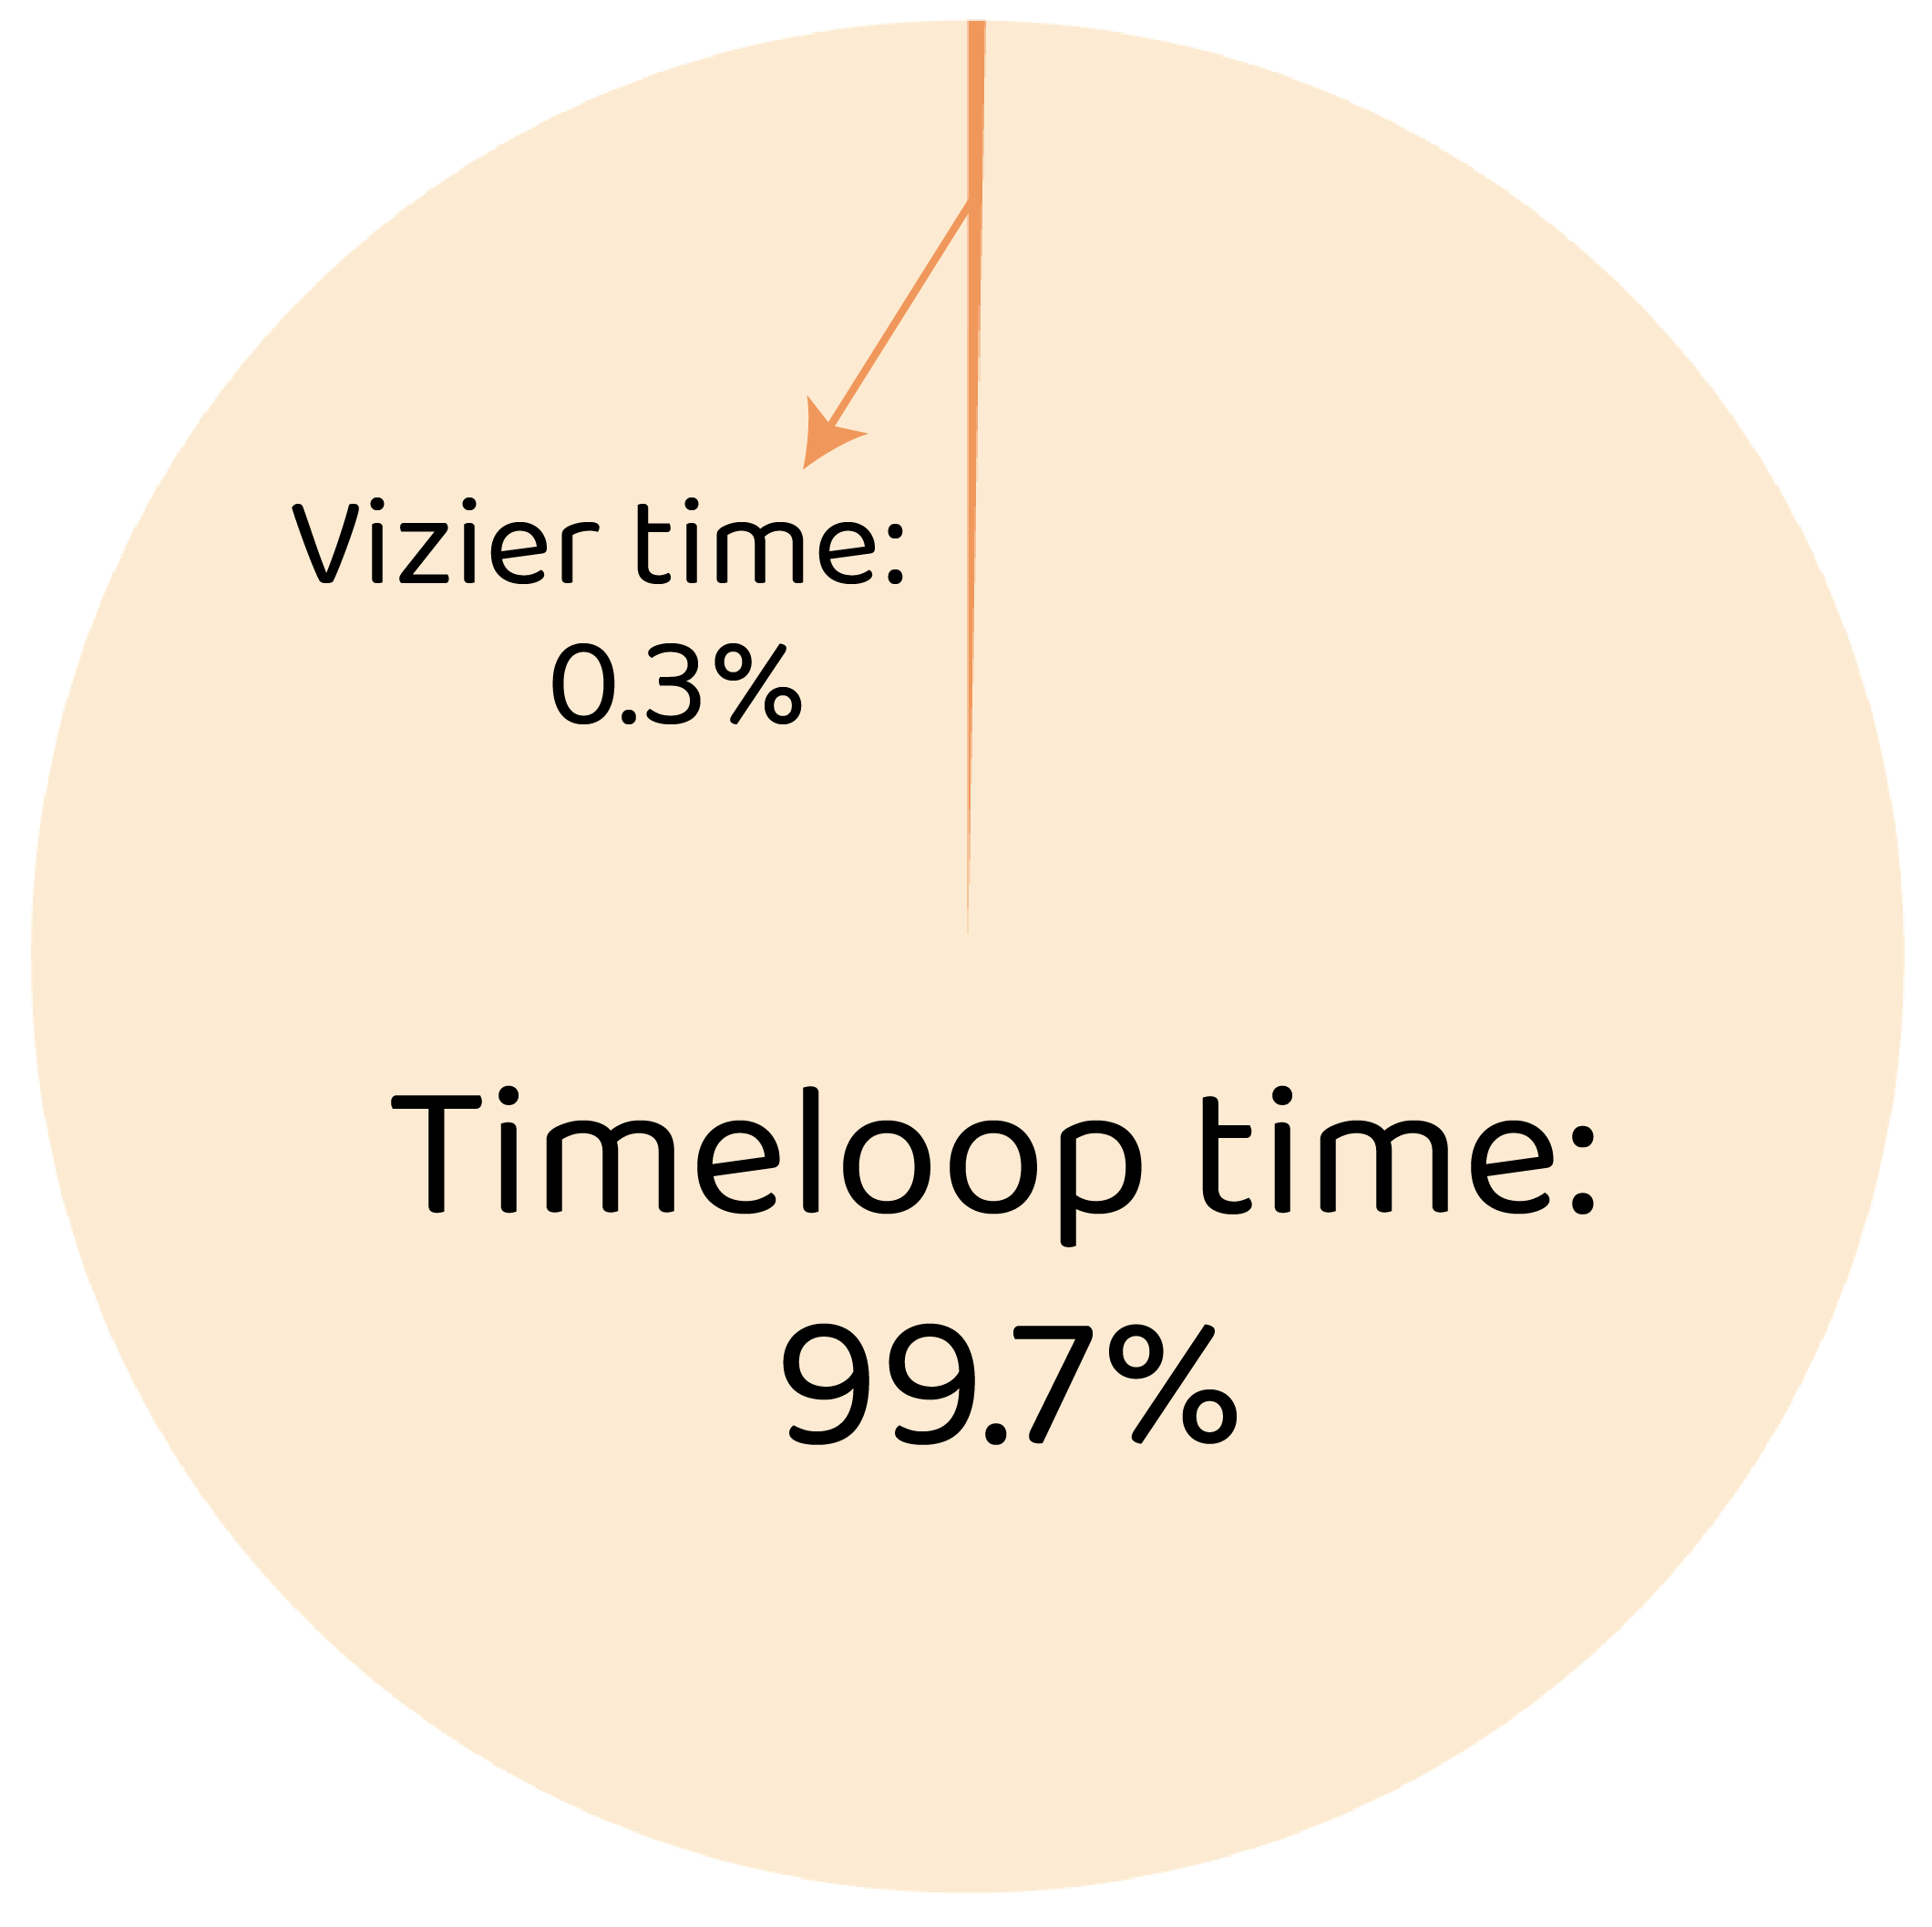
\includegraphics[width=\linewidth]{fig3/timeloop_vs_vizier.png}
% %     \caption{Per-trial wall-clock breakdown.}
% %     \label{fig:timeloop-time}
% %     \vspace{-10pt}
% % \end{wrapfigure}
% % Despite V0's improvements, it inherits the sequential dependence on external tiling tools (e.g., Timeloop) because it lacks a linear expression for non-linear tiling-fusion interactions. As shown in Figure~\ref{fig:timeloop-time}, Timeloop accounts for over 99\% of per-trial latency, creating a prohibitive bottleneck for multi-thousand-trial searches. To resolve this, CHEETAH-V1 internalizes tiling by precomputing Pareto-pruned configurations and encoding them as decision variables. This removes Timeloop from the critical path, collapsing each trial to a single Vizier-proposal and LP-solve step. We start with introducing the preprocessing stage below before presenting the full formulation in Section~\ref{sec::v1}.

% % % The limitations of prior work is still inherited in the V0 formulation due to the difficulty of expressing non-linear relationships as linear constraints. Therefore tiling decisions $(\Tmax_i, \Tmin_i, t_i^k)$ are fixed constants provided by additional software, such as Timeloop. A natural question is whether this sequential dependence also creates a \emph{runtime} bottleneck. Figure~\ref{fig:timeloop-time} confirms that it does: across different models, Timeloop scheduling on average accounts for over 99\% of per-trial wall-clock time, while the Vizier proposal and fusion ILP together consume less than 1\% on average. Because the outer loop requires thousands of trials to converge, the cumulative cost of repeated Timeloop invocations dominates the total search budget. This observation motivates a key design choice in CHEETAH-V1: rather than calling Timeloop online during each trial, we precompute a Pareto-pruned set of tiling configurations once (Section~\ref{sec:pareto}) and encode the tiling selection as decision variables \emph{inside} the LP. This eliminates Timeloop from the per-trial critical path entirely, reducing each trial to a single Vizier-proposal$\,\to\,$LP-solve step.

% % % CHEETAH-V1 captures tiling as a \emph{decision variable} inside the LP, enabling the solver to jointly optimize tiling and fusion. We start with describing our preprocessing stage in Section~\ref{sec:pareto} before presenting the full formulation in Section~\ref{sec::v1}.


% % \paragraph{Pareto Pruning Pre-Pass} The raw tiling search space for a $7$-dimensional convolution loop with $3$ memory levels is $\mathcal O(10^7)$ configurations per operation. We reduce this to a tractable Pareto-optimal subset $\mathcal{C}_i$ for each operation $i$ via a pre-pass for (1) L1 feasibility where configurations whose tiled working set exceeds L1 scratchpad capacity $C_{L1}$ are discarded; (2) Pareto optimality where a configuration $c$ is retained only if no other configuration achieves both lower $\Tmax_i(c)$ \emph{and} smaller working-set size in the Global Buffer.

% % In practice, Pareto pruning reduces $\mathcal O(10^7)$ raw configurations to $|\mathcal{C}_i| \approx 10^2$ to $10^3$ per operation. Timeloop is run once per (operation, configuration) pair, producing the triple $(\Tmin_i(c), \Tmax_i(c), t_i^k(c))$ for each retained configuration $c \in \mathcal{C}_i$. These are precomputed constants---the LP solver makes no Timeloop calls at solve time.

% % \paragraph{Time-invariant Pareto fronts.}
% % A key observation is that the Pareto front shape is invariant to memory time: configurations are ranked by compute cycles and working-set bytes, neither of which depends on bandwidth. Changing bandwidth rescales the DRAM access cost $t_i^k(c)$ uniformly. This means the Pareto-pruned configuration sets can be precomputed \emph{once} and reused across all Vizier trials that share the same compute configuration class, amortizing the expensive Timeloop precomputation.

% % \subsubsection{The Joint CHEETAH-V1 LP Formulation}\label{sec::v1}

% % \paragraph{From fixed constants to decision variables.}
% % In static and V0 formulations, Timeloop selects a single tiling per operation externally and passes the results to the LP as fixed constants $\Tmax_i$, $\Tmin_i$, $t_i^k$. The DRAM savings from pinning tensor $k$ of operation $i$ is then simply $t_i^k \cdot p_{i,o(i)}^k$---a constant times a variable, which is already linear. V1 brings this tiling choice \emph{inside} the LP by introducing \textbf{tiling selection variables} $y_{i,c} \in [0,1]$, one per Pareto-optimal configuration $c \in \mathcal{C}_i$ from the pre-pass, with the constraint $\sum_c y_{i,c} = 1$ (exactly one configuration is selected per operation). The Timeloop-precomputed constants $\Tmax_i(c)$, $\Tmin_i(c)$, $t_i^k(c)$ now become \emph{per-configuration coefficients} indexed by $c$. This means the DRAM savings term becomes $t_i^k(c) \cdot y_{i,c} \cdot p_{\text{assoc}(i,k),\, o(i)}$. This is a product of \emph{two} decision variables, which is bilinear and cannot be handled by a convex programming directly.
 
% % % \paragraph{Linearization via McCormick envelopes.}
% % % We linearize this product exactly via the classical McCormick substitution. Specifically,  we introduce \textbf{auxiliary variables} $w_{i,c,k} := y_{i,c} \cdot p_{\text{assoc}(i,k),\, o(i)}$ that represent the joint effect of selecting tiling $c$ \emph{and} pinning tensor $k$, constrained by:
% % % \begin{equation}
% % % \label{eq:mccormick}
% % % \begin{aligned}
% % %     w_{i,c,k} &\leq y_{i,c}, \qquad
% % %     w_{i,c,k} \leq p_{\text{assoc}(i,k),\, o(i)} \\
% % %     w_{i,c,k} &\geq y_{i,c} + p_{\text{assoc}(i,k),\, o(i)} - 1, \qquad
% % %     w_{i,c,k} \geq 0
% % % \end{aligned}
% % % \end{equation}
% % % Since both factors lie in $[0,1]$, these four constraints force $w_{i,c,k} = y_{i,c} \cdot p$ at any integer vertex, requiring no manually tuned constants. Together, $y_{i,c}$ and $w_{i,c,k}$ account for 1.6M of the 2.08M variables in the \Vone~ LP (Table~\ref{tab:v1_scale}). \todo{change to MoE?}

% % \paragraph{Linearization via McCormick envelopes.}
% % We linearize this product exactly via the classical McCormick substitution \citep{mccormick1976computability}. Specifically, we introduce \textbf{auxiliary variables} $w_{i,c,k} := y_{i,c} \cdot p_{\text{assoc}(i,k),\, o(i)}$ that represent the joint effect of selecting tiling $c$ \emph{and} pinning tensor $k$, constrained by:
% % \begin{equation}
% % \label{eq:mccormick}
% % \begin{aligned}
% %     w_{i,c,k} &\leq y_{i,c}, \qquad
% %     w_{i,c,k} \leq p_{\text{assoc}(i,k),\, o(i)} \\
% %     w_{i,c,k} &\geq y_{i,c} + p_{\text{assoc}(i,k),\, o(i)} - 1, \qquad
% %     w_{i,c,k} \geq 0
% % \end{aligned}
% % \end{equation}
% % Since both factors lie in $[0,1]$, these four constraints force $w_{i,c,k} = y_{i,c} \cdot p$ at any integer vertex, requiring no manually tuned constants. Together, $y_{i,c}$ and $w_{i,c,k}$ constitute the majority of V1's decision variables (Table~\ref{tab:v1_scale}).
 

% % % \paragraph{Full formulation.}
% % % Combining tiling selection, time-indexed placement, rematerialization, and McCormick linearization, the full V1  formulation is:

% % % \begin{equation}
% % % % \label{eq:v1}
% % % \begin{aligned}
% % % \min \quad & \sum_{i \in \mathcal{N}} T_i + \sum_{i \in \mathcal{N}} \sum_{t \in \mathcal{T}} c_i^{\text{remat}} \, r_{i,t} \\[4pt]
% % % \text{s.t.} \quad
% % % & \sum_{c \in \mathcal{C}_i} y_{i,c} = 1 & \forall\, i \in \mathcal{N} \\[3pt]
% % % & T_i \geq \sum_{c \in \mathcal{C}_i} \Tmax_i(c)\, y_{i,c} - \sum_{c \in \mathcal{C}_i} \sum_{k} t_i^k(c)\, w_{i,c,k} & \forall\, i \in \mathcal{N} \\[3pt]
% % % & T_i \geq \sum_{c \in \mathcal{C}_i} \Tmin_i(c)\, y_{i,c} & \forall\, i \in \mathcal{N} \\[3pt]
% % % & w_{i,c,k} \leq y_{i,c} & \forall\, i, c, k \\
% % % & w_{i,c,k} \leq p_{\text{assoc}(i,k),\, o(i)} & \forall\, i, c, k \\
% % % & w_{i,c,k} \geq y_{i,c} + p_{\text{assoc}(i,k),\, o(i)} - 1 & \forall\, i, c, k \\[3pt]
% % % & \sum_{e \in \mathcal{E}} d_e\, p_{e,t} + \sum_{i \in \mathcal{N}} d_i^W\, p_{i,t}^W \leq \CGM & \forall\, t \in \mathcal{T} \\[3pt]
% % % & p_{e,t} \leq p_{e,t-1} + r_{\text{src}(e),\, t} & \forall\, e, t > o(\text{src}(e)) \\
% % % & p_{i,t}^W \leq p_{i,t-1}^W & \forall\, i, t > o(i) \\[3pt]
% % % & r_{i,t} = 0 & \forall\, i, t \leq o(i) \\
% % % & r_{i,t} \leq p_{e,t} & \forall\, e \in \text{in}(i), t > o(i) \\
% % % & r_{i,t} \leq p_{i,t}^W & \forall\, i, t > o(i) \\[3pt]
% % % & T_i, p_{e,t}, p_{i,t}^W, r_{i,t}, w_{i,c,k} \geq 0 &
% % % \end{aligned}
% % % \tag{\textcolor{skyblue}{V1}}\label{eq:v1}
% % % \end{equation}
% % % full formulation below in appendix 
% % % \begin{equation}
% % % \begin{aligned}
% % % \min \quad & \sum_{i \in \mathcal{N}} T_i + \sum_{i \in \mathcal{N}} \sum_{t \in \mathcal{T}} c_i^{\text{remat}} \, r_{i,t} \\[4pt]
% % % \text{s.t.} \quad
% % % & \sum_{c \in \mathcal{C}_i} y_{i,c} = 1 & \forall\, i \in \mathcal{N} \\[3pt]
% % % & T_i \geq \max\!\left(\sum_{c \in \mathcal{C}_i} \Tmin_i(c)\, y_{i,c},\;\; \sum_{c \in \mathcal{C}_i} \Tmax_i(c)\, y_{i,c} - \sum_{c \in \mathcal{C}_i} \sum_{k} t_i^k(c)\, w_{i,c,k}\right) & \forall\, i \in \mathcal{N} \\[3pt]
% % % & w_{i,c,k} \leq y_{i,c}, \quad w_{i,c,k} \leq p_{\text{assoc}(i,k),\, o(i)}, \quad w_{i,c,k} \geq y_{i,c} + p_{\text{assoc}(i,k),\, o(i)} - 1 & \forall\, i, c, k \\[3pt]
% % % & \sum_{e \in \mathcal{E}} d_e\, p_{e,t} + \sum_{i \in \mathcal{N}} d_i^W\, p_{i,t}^W \leq \CGM & \forall\, t \in \mathcal{T} \\[3pt]
% % % & p_{e,t} \leq p_{e,t-1} + r_{\text{src}(e),\, t} & \forall\, e,\, t > o(\text{src}(e)) \\
% % % & p_{i,t}^W \leq p_{i,t-1}^W & \forall\, i,\, t > o(i) \\[3pt]
% % % & r_{i,t} = 0 \;\; \forall\, t \leq o(i); \quad r_{i,t} \leq \min\!\big(p_{e,t},\, p_{i,t}^W\big) \;\; \forall\, e \in \text{in}(i),\, t > o(i) \\[3pt]
% % % & T_i,\, p_{e,t},\, p_{i,t}^W,\, r_{i,t},\, w_{i,c,k} \geq 0 &
% % % \end{aligned}
% % % \tag{\textcolor{skyblue}{V1}}\label{eq:v1}
% % % \end{equation}

% % \paragraph{Variable and constraint digest.}
% % The V1 formulation inherits all the features of the V0 formulation, and additionally captures tiling by introducing selection variables
% % $y_{i,c} \in [0,1]$, constrained by $\sum_c y_{i,c} = 1$, to choose
% % from $|\mathcal{C}_i|$ Pareto-optimal configurations.
% % Each configuration defines compute costs $T_i^{\max}(c)$,
% % $T_i^{\min}(c)$, and per-tensor DRAM savings $t_i^k(c)$.
% % We linearize the resulting bilinear DRAM-savings term exactly via
% % McCormick auxiliary variables $w_{i,c,k}$, which enforce $w_{i,c,k} \;=\; y_{i,c} \cdot p_{\mathrm{assoc}(i,k),\,o(i)}$ at integer vertices without a relaxation gap.

% % Per-operation latency $T_i$ is lower-bounded by the weighted
% % configuration floor $\sum_c T_i^{\min}(c)\, y_{i,c}$ and the weighted
% % off-chip cost $\sum_c T_i^{\max}(c)\, y_{i,c}$ minus achievable savings
% % $\sum_{c,k} t_i^k(c)\, w_{i,c,k}$.
% % This coupling enables the solver to accept sub-optimal local tiling
% % (higher $T_i^{\max}$) if its smaller memory footprint unlocks global
% % fusion gains that outweigh the compute-utilization loss.
% % Capacity and persistence constraints carry over from V0, utilizing
% % edge-indexed placement $p_{e,t}$ to handle multi-fanout nodes.
% % For DeepSeek-V3, the V1 LP scales to approximately $2{,}504{,}019$ variables, $2{,}983{,}450$ constraints, and $6{,}094{,}156$ non-zeros. Table~\ref{tab:v1_scale} provides a representative breakdown, Table~\ref{tab:comparison} summarizes features of each more powerful formulation; full per-model sizes are in Table~\ref{tab:exp1_lp_sizes} and \ref{tab:exp2_cluster_lp_sizes}. 



% % % The V1 formulation extends V0 by making the tiling configuration a decision variable. The selection variables $y_{i,c} \in [0,1]$, with $\sum_c y_{i,c} = 1$, choose among $|\mathcal{C}_i|$ Pareto-optimal tiling configurations precomputed by Timeloop (Section~\ref{sec:pareto}). Each configuration $c$ determines the operation's compute cost $T_i^{\max}(c)$, on-chip floor $T_i^{\min}(c)$, and per-tensor DRAM savings $t_i^k(c)$.
% % % The DRAM savings term $t_i^k(c) \cdot y_{i,c} \cdot p_{\text{assoc}(i,k),\,o(i)}$ 
% % % is bilinear in the tiling selection and placement variables; we linearize it 
% % % via McCormick auxiliary variables $w_{i,c,k}$, constrained by 
% % % $w_{i,c,k} \leq y_{i,c}$, $w_{i,c,k} \leq p_{\text{assoc}(i,k),\,o(i)}$, and 
% % % $w_{i,c,k} \geq y_{i,c} + p_{\text{assoc}(i,k),\,o(i)} - 1$. 
% % % These three inequalities force $w_{i,c,k} = y_{i,c} \cdot p_{\text{assoc}(i,k),\,o(i)}$ 
% % % at any integer-feasible point (\cref{prop:mccormick_exact}), so the LP exactly captures the 
% % % bilinear interaction without introducing any relaxation gap at integer vertices.
% % % The $T_i$ lower bound now takes the maximum of two configuration-dependent terms: the weighted on-chip floor $\sum_c T_i^{\min}(c)\, y_{i,c}$ and the weighted off-chip cost minus achievable savings $\sum_c T_i^{\max}(c)\, y_{i,c} - \sum_{c,k} t_i^k(c)\, w_{i,c,k}$.
% % % This coupling is the core novelty of V1: the solver can accept a tiling with higher $T_i^{\max}(c)$ (lower compute utilization) if its smaller working set enables pinning decisions that reduce total DRAM traffic by more than the utilization loss.
% % % All remaining constraints---memory capacity, persistence, and rematerialization---carry over from V0 with edge-indexed placement variables $p_{e,t}$ replacing per-tensor $p_{i,t}^k$ to correctly handle skip connections and multi-fanout nodes. For our largest workload, DeepSeek-V3 ($L \approx 6{,}300$ operations), the V1 LP contains approximately 2.5M variables, 3.0M constraints, and 6.1M nonzeros. Table~\ref{tab:v1_scale} provides a representative breakdown; full per-model sizes are in Table~\ref{tab:v1_scale}. 
% % % \paragraph{Key constraint interactions.}
% % % The execution-time constraints (lines 2--3: the upper and lower bounds for $T_i$) capture the central trade-off that is unique to \Vone: the LP must commit to a tiling configuration $c$ (via $y_{i,c}$) that sets both the baseline compute cost $\Tmax_i(c)$ and the achievable DRAM savings $t_i^k(c)$. A configuration with smaller tiles may have higher $\Tmax_i(c)$ (lower compute utilization) but smaller working sets, enabling more aggressive pinning. The LP balances these trade-offs simultaneously---precisely the cross-stage interaction that the sequential pipeline cannot discover.
 
% % % The edge-indexed persistence constraint (line 8: $p_{e,t} \leq p_{e,t-1} + r_{\text{src}(e),\, t}$) and the memory capacity constraint (line 7: lower bound on $\CGM$) are inherited from \Vzero, which introduced per-edge placement variables $p_{e,t}$ to correctly model skip connections. \Vone~ extends this by coupling edge sizes to the tiling selection---since different configurations $c$ produce different activation working sets, the LP can now jointly reason about how tiling choices affect memory pressure across skip connections.


% % \begin{figure}[ht!]
% % \begin{minipage}[t]{0.48\textwidth}
% % \vspace{0pt}
% % \centering
% % \captionof{table}{V1 variable and constraint counts
% % (representative, DeepSeek-V3).}
% % \label{tab:v1_scale}
% % \footnotesize
% % \begin{tabular}{@{}ll@{}}
% % \toprule
% % \textbf{Variable} & \textbf{Role} \\
% % \midrule
% % $T_i$       & Per-operation execution time \\
% % $y_{i,c}$   & Tiling config selection ($|\mathcal{C}_i|$ options) \\
% % $p_{e,t}$   & Edge-indexed activation placement \\
% % $p_{i,t}^W$ & Weight placement \\
% % $r_{i,t}$   & Rematerialization indicator \\
% % $w_{i,c,k}$ & McCormick auxiliaries ($y_{i,c} \cdot p$) \\
% % % \midrule
% % % \multicolumn{2}{@{}l}{\textbf{DeepSeek-V3 totals}
% % %                        ($L \approx 6{,}300$)} \\
% % % \midrule
% % % Variables   & $2{,}504{,}019$ \\
% % % Constraints & $2{,}983{,}450$ \\
% % % Nonzeros    & $6{,}094{,}156$ \\
% % \bottomrule
% % \end{tabular}
% % \end{minipage}%
% % \hspace{0.02\textwidth}%
% % \begin{minipage}[t]{0.48\textwidth}
% % \vspace{0pt}
% % \centering
% % \captionof{table}{Comparison of static, V0, and V1 formulations.}
% % \label{tab:comparison}
% % \footnotesize
% % \begin{tabular}{@{}lccc@{}}
% % \toprule
% % \textbf{Property} & \textbf{Static} & \textbf{V0} & \textbf{V1} \\
% % \midrule
% % Joint tiling + fusion    & $\times$ & $\times$   & \checkmark \\
% % Time-indexed placement   & $\times$ & \checkmark & \checkmark \\
% % Rematerialization        & $\times$ & \checkmark & \checkmark \\
% % Relaxed skip connections & $\times$ & Partial    & \checkmark \\
% % \bottomrule
% % \end{tabular}

% % \medskip
% % \raggedright
% % \footnotesize
% % % \textbf{Comparison across formulations.}
% % % Table~\ref{tab:comparison} summarizes the progression from the
% % % static formulation through V0 to V1.
% % \end{minipage}
% % \end{figure}


% % % \begin{table}[ht!]
% % % \centering
% % % \caption{V1 variable and constraint counts (representative, DeepSeek-V3).}
% % % \label{tab:v1_scale}
% % % \small
% % % \begin{tabular}{lrl}
% % % \toprule
% % % \textbf{Variable} & \textbf{Role} \\
% % % \midrule
% % % $T_i$ & Per-operation execution time \\
% % % $y_{i,c}$ & Tiling configuration selection ($|\mathcal{C}_i|$ options per op) \\
% % % $p_{e,t}$ & Edge-indexed activation placement \\
% % % $p_{i,t}^W$ & Weight placement \\
% % % $r_{i,t}$ & Rematerialization indicator \\
% % % $w_{i,c,k}$ & McCormick auxiliaries ($y_{i,c} \cdot p$) \\
% % % \midrule
% % % \multicolumn{2}{l}{\textbf{DeepSeek-V3 totals} ($L \approx 6{,}300$)} \\
% % % \midrule
% % % Variables & 2,504,019 \\
% % % Constraints & 2,983,450 \\
% % % Nonzeros & 6,094,156 \\
% % % \bottomrule
% % % \end{tabular}
% % % \end{table}
% % % \paragraph{Comparison across formulations.}
% % % Table~\ref{tab:comparison} summarizes the progression from static through V0 to V1.
% % % \begin{table}[ht!]
% % % \centering
% % % \caption{Comparison of static, V0, and V1 formulations.}
% % % \label{tab:comparison}
% % % \small
% % % \begin{tabular}{lccc}
% % % \toprule
% % % \textbf{Property} & \textbf{static} & \textbf{V0} & \textbf{V1} \\
% % % \midrule
% % % Joint tiling + fusion & \texttimes & \texttimes & \checkmark \\
% % % Time-indexed placement & \texttimes & \checkmark & \checkmark \\
% % % Rematerialization & \texttimes & \checkmark & \checkmark \\
% % % Relaxed skip connections & \texttimes & Partial & \checkmark \\
% % % % Config-dependent DRAM savings & \texttimes & \texttimes & \checkmark \\ 
% % % % Bilinear linearization & --- & --- & McCormick \\
% % % \bottomrule
% % % \end{tabular}
% % % \end{table}

% % % \paragraph{Structural invariance for efficient LLM integration.}
% % % A practical advantage of both our LP formulations is that the constraint matrix sparsity pattern is invariant across hardware configurations---only the numerical coefficients change. This means:
% % % \begin{itemize}
% % %     \item The LP solver's preconditioner can be designed once per neural network model and reused across all Vizier trials.
% % %     \item An LLM-Architect can reason about constraint structure (which constraints are binding, which variables are fractional) without needing to understand the full LP.
% % %     \item Warm-starting from a previous trial's LP solution is straightforward since the variable indexing is stable.
% % % \end{itemize}

% % \subsection{Strategic Intelligence: LLM-Guided Outer Search}
% % \label{sec:llm_outer}
% % We use Google Vizier as a black-box Bayesian optimizer to propose hardware configurations. While effective, vanilla Vizier treats search as pure function optimization, often requiring thousands of iterations to identify suboptimal regions without leveraging structural hardware-workload knowledge. To address this, we introduce an LLM-guided outer-loop controller based on SkyDiscovery that reasons about co-design decisions. By learning from a causal ledger of past trials and Lagrangian dual signals from the LP solver, the LLM proposes meaningful, constrained search-space candidates. This integration is enabled by the CHEETAH-V1 formulation, which removes the Timeloop bottleneck to reduce trial times from days to hours.The LLM-Architect reduces wasted trials by intelligently steering Vizier’s search without altering the inner solver or its optimality certificates. In this hybrid loop, the LLM determines global architectural regions, Vizier performs local Bayesian optimization within those patches, and the large-scale V1 LP solver evaluates each concrete candidate. The LLM-Architect loop proceeds as follows: 
% % % We use Vizier as a black-box Bayesian optimizer to propose candidate hardware configurations. While effective, Vizier search strategies (LCS, UCB, etc) requires thousands of iterations explore and learn which regions are suboptimal and treats the search as a pure function optimization problem without leveraging structural knowledge about hardware-workload interactions.
% % % We leverage an LLM-guided outer-loop controller that learns from logs of thousands of past co-design trials to propose meaningful search-space candidates for Vizier. This is a SkyDiscovery based outer LLM layer which reasons about hardware-software co-design decisions and learns from a causal ledger of constantly updated logs across trials, as well as feed-back signal such as dual variables through the LP solve. This is possible for CHEETAH-V1 LP formulation, since it removes the Timeloop-in-the-loop constraint, thus reducing the co-design problem from days to hours, and permitting the LLM outer loop. 

% % % The LLM-Architect does not change the inner solver, and retains all the optimal certificates of the V1 LP formulation, but intelligently changes where the Vizier outer hardware optimizer searches to reduce wasted trials. The LLM proposes global decisions to determine constrained regions of the hardware search space; Vizier then performs local Bayesian optimization inside those regions; which then passes downstream into a large scale LP solver for the V1 formulation to evaluate each concrete candidate. The LLM-Architect loop proceeds as follows:

% % \begin{enumerate}[leftmargin=1.6em, itemsep=4pt]

% % \item \textbf{Extraction.}
% % Deterministic scripts summarize recent trials into a \emph{Causal
% % Ledger}. Each record includes hardware parameters, validity, Perf/TDP,
% % LP cycles, capacity duals/slacks, bandwidth sensitivity, MFU, memory
% % utilization, roofline gap, failure class, and LP solver metrics.

% % \item \textbf{Context building.}
% % The last $N$ trials and the Causal Ledger are compressed into a compact
% % JSON context for the Architect. The context emphasizes empirical
% % feasibility, observed invalid regions, best known valid designs, and
% % physical audit signals.

% % \item \textbf{Architect.}
% % The online Architect, implemented as Qwen2.5-7B-Instruct with a LoRA
% % adapter trained on past trial logs, diagnoses the dominant bottleneck
% % and emits a campaign patch. The patch constrains macro-architectural
% % search decisions such as Global Memory, DRAM bandwidth, total MACs,
% % systolic shape, PE grid, and batch size. A larger teacher model,
% % DeepSeek-V3.2, was used offline to generate or critique campaign labels
% % but is not in the live loop.

% % \item \textbf{Campaign validation.}
% % A deterministic validator clips or rejects the LLM patch to enforce
% % legal hardware ranges, TDP and area limits, MAC caps, CGM feasibility
% % floors, compute/bandwidth coupling, and roofline constraints. This
% % prevents the LLM from proposing physically implausible regions such as
% % maximum-MAC/minimum-bandwidth designs.

% % \item \textbf{Local optimization.}
% % Vizier is initialized inside the validated patch and warm-started with
% % prior trials that lie in the same region. Vizier then samples concrete
% % hardware candidates within the approved campaign. The LLM therefore
% % chooses the high-level architectural neighbourhood, while Vizier
% % performs local adaptive optimization.

% % \item \textbf{Unified V1 evaluation.}
% % The large-scale LP solver evaluates each candidate by solving the V1
% % joint tiling-fusion-placement LP using saved Pareto $\mathcal{C}$-sets.
% % It returns the objective, cycles, selected tiling configurations,
% % placement/rematerialization decisions, dual/slack summaries, and
% % solver-quality diagnostics.

% % \item \textbf{Roofline audit.}
% % A deterministic Roofline Auditor checks whether the predicted latency
% % is physically plausible. For each candidate we compute
% % \begin{align}
% %     t_{\text{compute}} &=
% %         \frac{\text{useful FLOPs}}{\text{peak FLOPs/s}},
% %     \qquad
% %     t_{\text{memory}}  =
% %         \frac{\text{post-placement DRAM bytes}}{\text{peak bandwidth}},
% %     \nonumber\\
% %     t_{\text{ideal}}   &=
% %         \max\!\left(t_{\text{compute}},\, t_{\text{memory}}\right).
% %     \label{eq:roofline_audit}
% % \end{align}
% % A candidate is rejected if the solver-reported latency falls below this
% % lower bound, or if MFU or memory utilization exceeds 1.0 within
% % tolerance.

% % \item \textbf{Ledger update.}
% % The loop records the campaign hypothesis, intervention, observed
% % invalid-rate change, MFU change, roofline validity, and best Perf/TDP
% % change. The ledger also records forbidden regions when a campaign
% % produces excessive invalid trials.

% % \end{enumerate}

% % \noindent The Architect receives workload summaries, invalid-rate
% % history, MFU, roofline signals, prior valid regions, normalized LP duals,
% % and bandwidth sensitivities. The system starts from a safe empirically
% % valid patch and permits duals only to make bounded edits, such as raising
% % the CGM floor, increasing bandwidth, reducing MAC count, or changing
% % systolic shapes. The validator rejects any dual-guided patch that
% % excludes known high-performing valid regions or predicts a substantially
% % worse feasible rate. This provides controlled architectural feedback in
% % addition to prompt input.


% % % \todo{Expand this section once the LLM+RL experimental protocol is finalized. Key questions to address: (1) Which LLM is used and how is it prompted? (2) How are LLM proposals integrated with Vizier's Bayesian model? (3) What is the sample efficiency improvement over pure Vizier?}





% % edit for page limit 
% \vspace{-0.4cm}
% \section{Methodology}
% \label{sec:methods}
% \vspace{-0.2cm}
% We present the CHEETAH (\acroletter{C}o-designed \acroletter{H}ardware \acroletter{E}xploration via \acroletter{E}fficient \acroletter{T}hroughput and \acroletter{H}ybrid-search) framework in three parts: Section~\ref{sec:v0} introduces CHEETAH-V0, which extends the static fusion ILP with time-indexed placement and rematerialization. Section~\ref{sec:v1} presents CHEETAH-V1, which jointly optimizes tiling and fusion via McCormick linearization. Section~\ref{sec:llm_outer} describes the LLM-Architect outer loop. Appendix~\ref{sec:theory} provides theoretical analysis on the exactness of our mathematical modeling, and Appendix~\ref{app:invar} provides details on structured constraint matrices.


% % \subsection{\Vzero~: Multi-Period Placement with Rematerialization}
% \subsection{CHEETAH-V0: Multi-Period Placement with Rematerialization}
% \label{sec:v0}

% Our first extension models the neural network's execution as a sequence of $T$ discrete timesteps (one per operation in execution order). This decides at which time, which tensor is pinned, evicted, or recomputed to optimally minimize cycle counts. The key features are:

% \paragraph{Time-indexed placement.}
% Instead of a single binary $p_i^k$ per tensor, we introduce $p_{i,t}^k \in [0,1]$ for each tensor $k$ of layer $i$ at each timestep $t$. A tensor can be pinned at timestep $t=5$, and evicted at $t=10$. This models a dynamic memory manager within a single inference pass.

% \paragraph{Rematerialization.}
% Rather than always paying DRAM bandwidth to reload an evicted tensor, we introduce variables $r_{i,t} \in [0,1]$ indicating that layer $i$ is recomputed at timestep $t$ to restore its output to the Global Buffer. This is particularly valuable for models such as EfficientNet, where depthwise convolutions account for only ${\sim}5\%$ of total FLOPs but produce large activation tensors. Recomputing a depthwise layer to avoid re-reading 6\,MiB from DRAM at 256\,GB/s can be faster than the DRAM reload itself.

% \paragraph{Relaxed skip-connection handling.}
% We lift the limitation of our baseline original ILP, which restricts activation pinning to consecutively-executed operations and limits multi-fanout nodes so that at most one consumer benefits from on-chip data. CHEETAH-V0 uses edge-indexed placement variables $p_{e,t}$ for each edge $e \in \mathcal{E}$ of the dataflow graph, correctly modeling the case where one consumer of a skip connection benefits from on-chip data while another does not.

% \vspace{-6pt}
% The CHEETAH-V0 LP formulation is:
% \begin{equation}
% % \label{eq:v0}
% \begin{aligned}
% \min \quad & \sum_{i \in \mathcal{N}} T_i + \sum_{i \in \mathcal{N}} \sum_{t \in \mathcal{T}} c_i^{\text{remat}} \, r_{i,t} \\
% \text{s.t.} \quad
% & T_i \geq \Tmax_i - \sum_{k \in \{I,O,W\}} t_i^k \cdot p_{i,o(i)}^k & \forall\, i \in \mathcal{N} \\
% & T_i \geq \Tmin_i & \forall\, i \in \mathcal{N} \\
% & \sum_{i \in \mathcal{N}} \sum_{k} d_i^k \, p_{i,t}^k \leq \CGM & \forall\, t \in \mathcal{T} \\
% & p_{i,t}^k \leq p_{i,t-1}^k + r_{i,t} & \forall\, i, t, k \in \{I,O\} \\
% & p_{i,t}^W \leq p_{i,t-1}^W & \forall\, i, t \\
% & r_{i,t} = 0 & \forall\, i, t \leq o(i) \\
% & 0 \leq p_{i,t}^k, r_{i,t} \leq 1 &
% \end{aligned}
% \tag{V0}\label{eq:v0}
% \end{equation}

% \vspace{-4pt}

% where $o(i)$ is the execution order of operation $i$, $d_i^k$ is the byte size of tensor $k$ for layer $i$, and $c_i^{\text{remat}}$ is the recomputation cost.

% \paragraph{Variable and constraint digest.}
% The objective minimizes total execution time $\sum_i T_i$ plus rematerialization costs. Per-operation latency $T_i$ is lower-bounded by the on-chip floor $T_i^{\min}$ and the off-chip time $T_i^{\max}$ adjusted for DRAM savings from pinned tensors. Persistence constraints enforce monotone eviction for weights and allow recomputation-based restoration for activations; rematerialization is only permitted post-execution and requires on-chip availability of both inputs and weights.
% For DeepSeek-V3 ($L \approx 6{,}300$), this formulation yields a large-scale program with approximately 3.3M variables and 3.7M constraints. See Appendix~\ref{sec:lps} for a detailed breakdown. 


% % \subsection{\textcolor{skyblue}{V1}: Joint Tiling and Fusion via McCormick Linearization}
% \vspace{-6pt}
% \subsection{CHEETAH-V1: Joint Tiling and Fusion via McCormick Linearization}
% \label{sec:v1}

% \begin{wrapfigure}{r}{0.2\linewidth}
%     \vspace{-12pt}
%     \centering
%     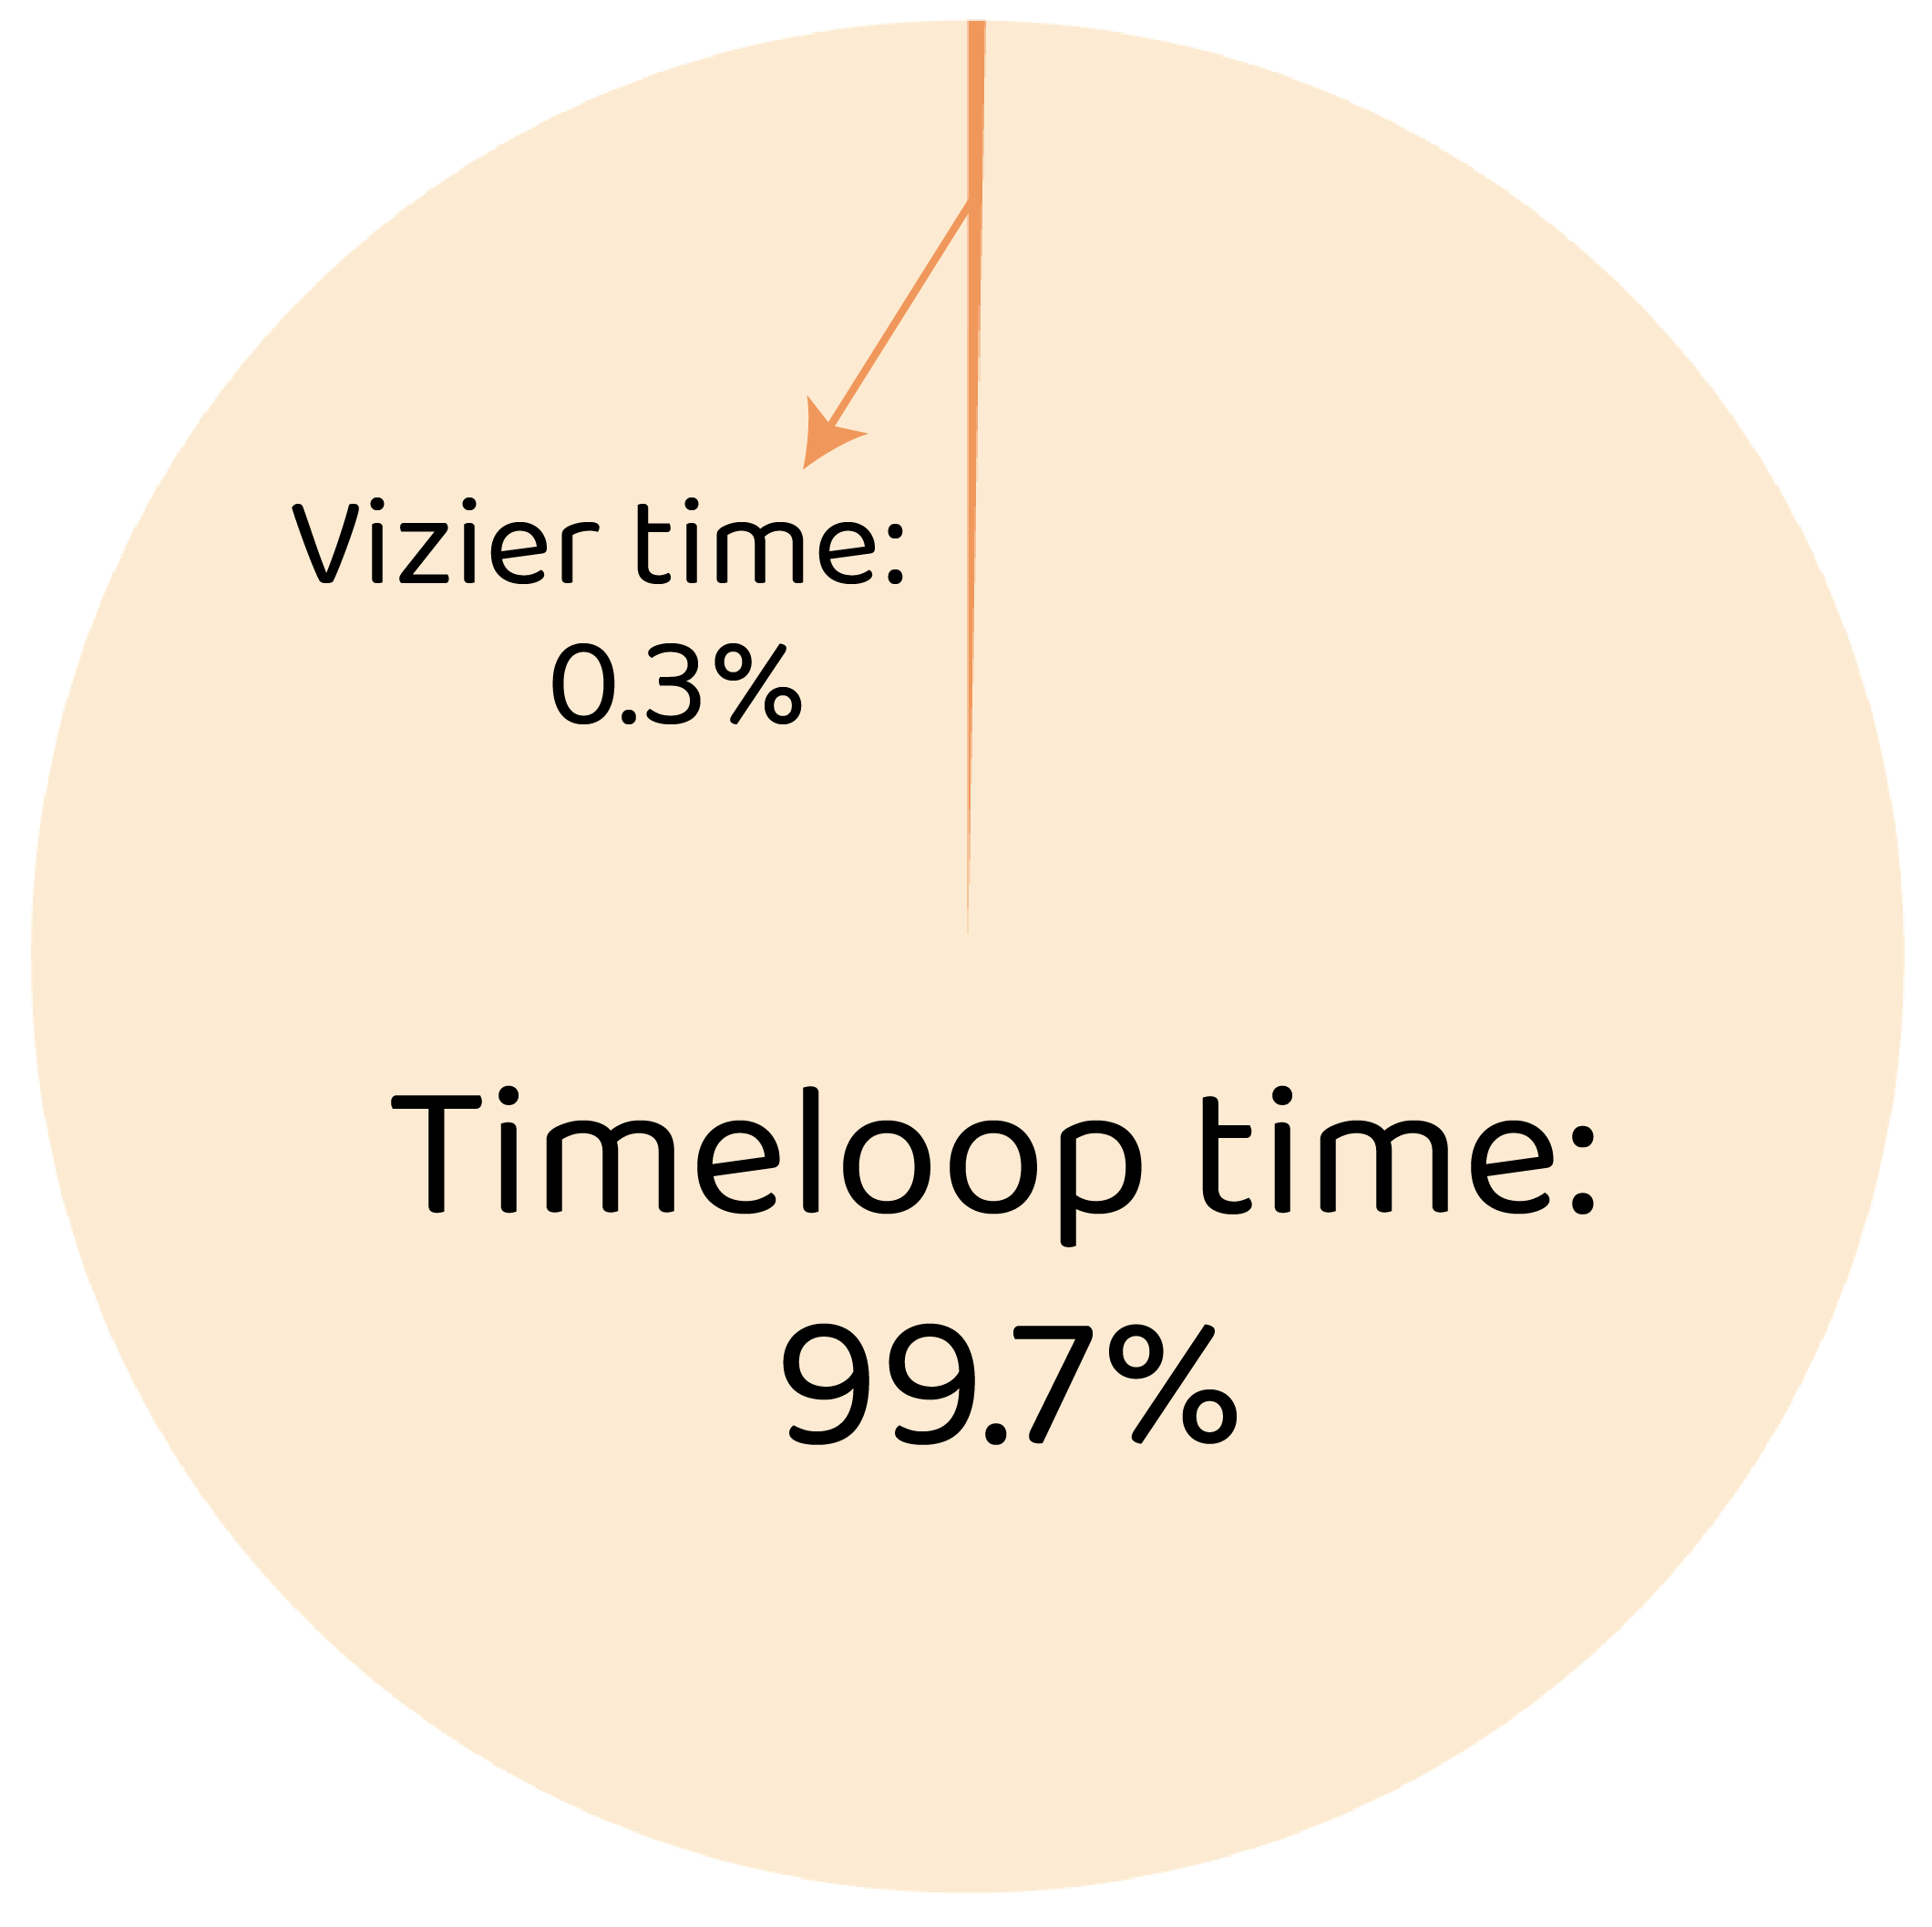
\includegraphics[width=\linewidth]{fig3/timeloop_vs_vizier.png}
%     \caption{Per-trial wall-clock breakdown.}
%     \label{fig:timeloop-time}
%     \vspace{-10pt}
% \end{wrapfigure}
% Despite V0's improvements, it inherits the sequential dependence on external tiling tools (e.g., Timeloop) because it lacks a linear expression for non-linear tiling-fusion interactions. As shown in Figure~\ref{fig:timeloop-time}, Timeloop accounts for over 99\% of per-trial latency, creating a prohibitive bottleneck for multi-thousand-trial searches. To resolve this, CHEETAH-V1 internalizes tiling by precomputing Pareto-pruned configurations and encoding them as decision variables. This removes Timeloop from the critical path, collapsing each trial to a single Vizier-proposal and LP-solve step. We start with introducing the preprocessing stage below before presenting the full formulation.

% % The limitations of prior work is still inherited in the V0 formulation due to the difficulty of expressing non-linear relationships as linear constraints. Therefore tiling decisions $(\Tmax_i, \Tmin_i, t_i^k)$ are fixed constants provided by additional software, such as Timeloop. A natural question is whether this sequential dependence also creates a \emph{runtime} bottleneck. Figure~\ref{fig:timeloop-time} confirms that it does: across different models, Timeloop scheduling on average accounts for over 99\% of per-trial wall-clock time, while the Vizier proposal and fusion ILP together consume less than 1\% on average. Because the outer loop requires thousands of trials to converge, the cumulative cost of repeated Timeloop invocations dominates the total search budget. This observation motivates a key design choice in CHEETAH-V1: rather than calling Timeloop online during each trial, we precompute a Pareto-pruned set of tiling configurations once (Section~\ref{sec:pareto}) and encode the tiling selection as decision variables \emph{inside} the LP. This eliminates Timeloop from the per-trial critical path entirely, reducing each trial to a single Vizier-proposal$\,\to\,$LP-solve step.

% % CHEETAH-V1 captures tiling as a \emph{decision variable} inside the LP, enabling the solver to jointly optimize tiling and fusion. We start with describing our preprocessing stage in Section~\ref{sec:pareto} before presenting the full formulation in Section~\ref{sec::v1}.


% \paragraph{Pareto Pruning Pre-Pass} The raw tiling search space for a $7$-dimensional convolution loop with $3$ memory levels is $\mathcal O(10^7)$ configurations per operation. We reduce this to a tractable Pareto-optimal subset $\mathcal{C}_i$ for each operation $i$ via a pre-pass for (1) L1 feasibility where configurations whose tiled working set exceeds L1 scratchpad capacity $C_{L1}$ are discarded; (2) Pareto optimality where a configuration $c$ is retained only if no other configuration achieves both lower $\Tmax_i(c)$ \emph{and} smaller working-set size in the Global Buffer.

% In practice, Pareto pruning reduces $\mathcal O(10^7)$ raw configurations to $|\mathcal{C}_i| \approx 10^2$ to $10^3$ per operation. Timeloop is run once per (operation, configuration) pair, producing the triple $(\Tmin_i(c), \Tmax_i(c), t_i^k(c))$ for each retained configuration $c \in \mathcal{C}_i$. These are precomputed constants---the LP solver makes no Timeloop calls at solve time. Appendix~\ref{app:details} provides more details.

% \paragraph{Time-invariant Pareto fronts.}
% A key observation is that the Pareto front shape is invariant to memory time: configurations are ranked by compute cycles and working-set bytes, neither of which depends on bandwidth. Changing bandwidth rescales the DRAM access cost $t_i^k(c)$ uniformly. This means the Pareto-pruned configuration sets can be precomputed \emph{once} and reused across all Vizier trials that share the same compute configuration class, amortizing the expensive Timeloop precomputation.

% % \subsubsection{The Joint CHEETAH-V1 LP Formulation}\label{sec::v1}

% \paragraph{From fixed constants to decision variables.}
% V1 brings the tiling choice \emph{inside} the LP by introducing \textbf{tiling selection variables} $y_{i,c} \in [0,1]$, one per Pareto-optimal configuration $c \in \mathcal{C}_i$ from the pre-pass, with the constraint $\sum_c y_{i,c} = 1$ (exactly one configuration is selected per operation). The Timeloop-precomputed constants $\Tmax_i(c)$, $\Tmin_i(c)$, $t_i^k(c)$ now become \emph{per-configuration coefficients} indexed by $c$, so the DRAM savings term becomes $t_i^k(c) \cdot y_{i,c} \cdot p_{\text{assoc}(i,k),\, o(i)}$---a product of \emph{two} decision variables, which is bilinear and cannot be handled by convex programming directly.
 
% % \paragraph{Linearization via McCormick envelopes.}
% % We linearize this product exactly via the classical McCormick substitution. Specifically,  we introduce \textbf{auxiliary variables} $w_{i,c,k} := y_{i,c} \cdot p_{\text{assoc}(i,k),\, o(i)}$ that represent the joint effect of selecting tiling $c$ \emph{and} pinning tensor $k$, constrained by:
% % \begin{equation}
% % \label{eq:mccormick}
% % \begin{aligned}
% %     w_{i,c,k} &\leq y_{i,c}, \qquad
% %     w_{i,c,k} \leq p_{\text{assoc}(i,k),\, o(i)} \\
% %     w_{i,c,k} &\geq y_{i,c} + p_{\text{assoc}(i,k),\, o(i)} - 1, \qquad
% %     w_{i,c,k} \geq 0
% % \end{aligned}
% % \end{equation}
% % Since both factors lie in $[0,1]$, these four constraints force $w_{i,c,k} = y_{i,c} \cdot p$ at any integer vertex, requiring no manually tuned constants. Together, $y_{i,c}$ and $w_{i,c,k}$ account for 1.6M of the 2.08M variables in the \Vone~ LP (Table~\ref{tab:v1_scale}). \todo{change to MoE?}

% \paragraph{Linearization via McCormick envelopes.}
% We linearize this product exactly via the classical McCormick substitution \citep{mccormick1976computability}. Specifically, we introduce \textbf{auxiliary variables} $w_{i,c,k} := y_{i,c} \cdot p_{\text{assoc}(i,k),\, o(i)}$ that represent the joint effect of selecting tiling $c$ \emph{and} pinning tensor $k$, constrained by:
% \vspace{-4pt}
% \begin{equation}
% \label{eq:mccormick}
% \begin{aligned}
%     w_{i,c,k} &\leq y_{i,c}, \qquad
%     w_{i,c,k} \leq p_{\text{assoc}(i,k),\, o(i)} \\
%     w_{i,c,k} &\geq y_{i,c} + p_{\text{assoc}(i,k),\, o(i)} - 1, \qquad
%     w_{i,c,k} \geq 0
% \end{aligned}
% \end{equation}
% Since both factors lie in $[0,1]$, these four constraints force $w_{i,c,k} = y_{i,c} \cdot p$ at any integer vertex, requiring no manually tuned constants. Together, $y_{i,c}$ and $w_{i,c,k}$ constitute the majority of V1's decision variables (Table~\ref{tab:v1_scale}).
% \vspace{-4pt}
% \paragraph{The Joint CHEETAH-V1 LP Formulation.}
% Combining tiling selection, time-indexed placement, rematerialization, and McCormick linearization, the full V1 formulation is:
% \begin{equation}
% \begin{aligned}
% \min \quad & \sum_{i \in \mathcal{N}} T_i + \sum_{i \in \mathcal{N}} \sum_{t \in \mathcal{T}} c_i^{\text{remat}} \, r_{i,t} \\[4pt]
% \text{s.t.} \quad
% & \sum_{c \in \mathcal{C}_i} y_{i,c} = 1 & \forall\, i \in \mathcal{N} \\[3pt]
% & T_i \geq \max\!\left(\sum_{c \in \mathcal{C}_i} \Tmin_i(c)\, y_{i,c},\;\; \sum_{c \in \mathcal{C}_i} \Tmax_i(c)\, y_{i,c} - \sum_{c \in \mathcal{C}_i} \sum_{k} t_i^k(c)\, w_{i,c,k}\right) & \forall\, i \in \mathcal{N} \\[3pt]
% & w_{i,c,k} \leq y_{i,c}, \quad w_{i,c,k} \leq p_{\text{assoc}(i,k),\, o(i)}, \quad w_{i,c,k} \geq y_{i,c} + p_{\text{assoc}(i,k),\, o(i)} - 1 & \forall\, i, c, k \\[3pt]
% & \sum_{e \in \mathcal{E}} d_e\, p_{e,t} + \sum_{i \in \mathcal{N}} d_i^W\, p_{i,t}^W \leq \CGM & \forall\, t \in \mathcal{T} \\[3pt]
% & p_{e,t} \leq p_{e,t-1} + r_{\text{src}(e),\, t} & \forall\, e,\, t > o(\text{src}(e)) \\
% & p_{i,t}^W \leq p_{i,t-1}^W & \forall\, i,\, t > o(i) \\[3pt]
% & r_{i,t} = 0 \;\; \forall\, t \leq o(i); \quad r_{i,t} \leq \min\!\big(p_{e,t},\, p_{i,t}^W\big) \;\; \forall\, e \in \text{in}(i),\, t > o(i) \\[3pt]
% & T_i,\, p_{e,t},\, p_{i,t}^W,\, r_{i,t},\, w_{i,c,k} \geq 0 &
% \end{aligned}
% \tag{V1}\label{eq:v1}
% \end{equation}

% \vspace{-4pt}



% \paragraph{Variable and constraint digest.}
% The V1 formulation inherits all the features of the V0 formulation, and additionally captures tiling by introducing selection variables
% $y_{i,c} \in [0,1]$, constrained by $\sum_c y_{i,c} = 1$, to choose
% from $|\mathcal{C}_i|$ Pareto-optimal configurations.
% Each configuration defines compute costs $T_i^{\max}(c)$,
% $T_i^{\min}(c)$, and per-tensor DRAM savings $t_i^k(c)$.
% We linearize the resulting bilinear DRAM-savings term exactly via
% McCormick auxiliary variables $w_{i,c,k}$, which enforce $w_{i,c,k} \;=\; y_{i,c} \cdot p_{\mathrm{assoc}(i,k),\,o(i)}$ at integer vertices without a relaxation gap. Appendix~\ref{app:lps} describes variables and constraints in detail.

% Per-operation latency $T_i$ is lower-bounded by the weighted
% configuration floor $\sum_c T_i^{\min}(c)\, y_{i,c}$ and the weighted
% off-chip cost $\sum_c T_i^{\max}(c)\, y_{i,c}$ minus achievable savings
% $\sum_{c,k} t_i^k(c)\, w_{i,c,k}$.
% This coupling enables the solver to accept sub-optimal local tiling
% (higher $T_i^{\max}$) if its smaller memory footprint unlocks global
% fusion gains that outweigh the compute-utilization loss.
% Capacity and persistence constraints carry over from V0, utilizing
% edge-indexed placement $p_{e,t}$ to handle multi-fanout nodes.
% For DeepSeek-V3, the V1 LP scales to approximately 2.5M variables,
% 3.0M constraints and 6.1M nonzeros. Table~\ref{tab:v1_scale} provides a representative breakdown; full per-model sizes are in Table~\ref{tab:exp1_lp_sizes} and \ref{tab:exp2_cluster_lp_sizes}. 



% % The V1 formulation extends V0 by making the tiling configuration a decision variable. The selection variables $y_{i,c} \in [0,1]$, with $\sum_c y_{i,c} = 1$, choose among $|\mathcal{C}_i|$ Pareto-optimal tiling configurations precomputed by Timeloop (Section~\ref{sec:pareto}). Each configuration $c$ determines the operation's compute cost $T_i^{\max}(c)$, on-chip floor $T_i^{\min}(c)$, and per-tensor DRAM savings $t_i^k(c)$.
% % The DRAM savings term $t_i^k(c) \cdot y_{i,c} \cdot p_{\text{assoc}(i,k),\,o(i)}$ 
% % is bilinear in the tiling selection and placement variables; we linearize it 
% % via McCormick auxiliary variables $w_{i,c,k}$, constrained by 
% % $w_{i,c,k} \leq y_{i,c}$, $w_{i,c,k} \leq p_{\text{assoc}(i,k),\,o(i)}$, and 
% % $w_{i,c,k} \geq y_{i,c} + p_{\text{assoc}(i,k),\,o(i)} - 1$. 
% % These three inequalities force $w_{i,c,k} = y_{i,c} \cdot p_{\text{assoc}(i,k),\,o(i)}$ 
% % at any integer-feasible point (\cref{prop:mccormick_exact}), so the LP exactly captures the 
% % bilinear interaction without introducing any relaxation gap at integer vertices.
% % The $T_i$ lower bound now takes the maximum of two configuration-dependent terms: the weighted on-chip floor $\sum_c T_i^{\min}(c)\, y_{i,c}$ and the weighted off-chip cost minus achievable savings $\sum_c T_i^{\max}(c)\, y_{i,c} - \sum_{c,k} t_i^k(c)\, w_{i,c,k}$.
% % This coupling is the core novelty of V1: the solver can accept a tiling with higher $T_i^{\max}(c)$ (lower compute utilization) if its smaller working set enables pinning decisions that reduce total DRAM traffic by more than the utilization loss.
% % All remaining constraints---memory capacity, persistence, and rematerialization---carry over from V0 with edge-indexed placement variables $p_{e,t}$ replacing per-tensor $p_{i,t}^k$ to correctly handle skip connections and multi-fanout nodes. For our largest workload, DeepSeek-V3 ($L \approx 6{,}300$ operations), the V1 LP contains approximately 2.5M variables, 3.0M constraints, and 6.1M nonzeros. Table~\ref{tab:v1_scale} provides a representative breakdown; full per-model sizes are in Table~\ref{tab:v1_scale}. 
% % \paragraph{Key constraint interactions.}
% % The execution-time constraints (lines 2--3: the upper and lower bounds for $T_i$) capture the central trade-off that is unique to \Vone: the LP must commit to a tiling configuration $c$ (via $y_{i,c}$) that sets both the baseline compute cost $\Tmax_i(c)$ and the achievable DRAM savings $t_i^k(c)$. A configuration with smaller tiles may have higher $\Tmax_i(c)$ (lower compute utilization) but smaller working sets, enabling more aggressive pinning. The LP balances these trade-offs simultaneously---precisely the cross-stage interaction that the sequential pipeline cannot discover.
 
% % The edge-indexed persistence constraint (line 8: $p_{e,t} \leq p_{e,t-1} + r_{\text{src}(e),\, t}$) and the memory capacity constraint (line 7: lower bound on $\CGM$) are inherited from \Vzero, which introduced per-edge placement variables $p_{e,t}$ to correctly model skip connections. \Vone~ extends this by coupling edge sizes to the tiling selection---since different configurations $c$ produce different activation working sets, the LP can now jointly reason about how tiling choices affect memory pressure across skip connections.




% % \centering
% % \caption{V1 variable and constraint counts (representative, DeepSeek-V3).}
% % \label{tab:v1_scale}
% % \small
% % \begin{tabular}{lrl}
% % \toprule
% % \textbf{Variable} & \textbf{Role} \\
% % \midrule
% % $T_i$ & Per-operation execution time \\
% % $y_{i,c}$ & Tiling configuration selection ($|\mathcal{C}_i|$ options per op) \\
% % $p_{e,t}$ & Edge-indexed activation placement \\
% % $p_{i,t}^W$ & Weight placement \\
% % $r_{i,t}$ & Rematerialization indicator \\
% % $w_{i,c,k}$ & McCormick auxiliaries ($y_{i,c} \cdot p$) \\
% % \midrule
% % \multicolumn{2}{l}{\textbf{DeepSeek-V3 totals} ($L \approx 6{,}300$)} \\
% % \midrule
% % Variables & 2,504,019 \\
% % Constraints & 2,983,450 \\
% % Nonzeros & 6,094,156 \\
% % \bottomrule
% % \end{tabular}
% % \end{table}
% % \paragraph{Comparison across formulations.}
% % Table~\ref{tab:comparison} summarizes the progression from static through V0 to V1.
% % \begin{table}[ht!]
% % \centering
% % \caption{Comparison of static, V0, and V1 formulations.}
% % \label{tab:comparison}
% % \small
% % \begin{tabular}{lccc}
% % \toprule
% % \textbf{Property} & \textbf{static} & \textbf{V0} & \textbf{V1} \\
% % \midrule
% % Joint tiling + fusion & \texttimes & \texttimes & \checkmark \\
% % Time-indexed placement & \texttimes & \checkmark & \checkmark \\
% % Rematerialization & \texttimes & \checkmark & \checkmark \\
% % Relaxed skip connections & \texttimes & Partial & \checkmark \\
% % % Config-dependent DRAM savings & \texttimes & \texttimes & \checkmark \\ 
% % % Bilinear linearization & --- & --- & McCormick \\
% % \bottomrule
% % \end{tabular}
% % \end{table}

% % \paragraph{Structural invariance for efficient LLM integration.}
% % A practical advantage of both our LP formulations is that the constraint matrix sparsity pattern is invariant across hardware configurations---only the numerical coefficients change. This means:
% % \begin{itemize}
% %     \item The LP solver's preconditioner can be designed once per neural network model and reused across all Vizier trials.
% %     \item An LLM-Architect can reason about constraint structure (which constraints are binding, which variables are fractional) without needing to understand the full LP.
% %     \item Warm-starting from a previous trial's LP solution is straightforward since the variable indexing is stable.
% % \end{itemize}

% \begin{wraptable}{r}{0.48\textwidth}
% \vspace{-12pt}   
% \centering
% \caption{V1 variable and constraint counts
% (representative, DeepSeek-V3).}
% \label{tab:v1_scale}
% \footnotesize
% \begin{tabular}{@{}ll@{}}
% \toprule
% \textbf{Variable} & \textbf{Role} \\
% \midrule
% $T_i$       & Per-operation execution time \\
% $y_{i,c}$   & Tiling config selection ($|\mathcal{C}_i|$ options) \\
% $p_{e,t}$   & Edge-indexed activation placement \\
% $p_{i,t}^W$ & Weight placement \\
% $r_{i,t}$   & Rematerialization indicator \\
% $w_{i,c,k}$ & McCormick auxiliaries ($y_{i,c} \cdot p$) \\
% \midrule
% \multicolumn{2}{@{}l}{\textbf{DeepSeek-V3 totals}
%                        ($L \approx 6{,}300$)} \\
% \midrule
% Variables   & $2{,}504{,}019$ \\
% Constraints & $2{,}983{,}450$ \\
% Nonzeros    & $6{,}094{,}156$ \\
% \bottomrule
% \end{tabular}
% \vspace{-14pt} 
% \end{wraptable}

% \vspace{-0.1cm}
% \subsection{Strategic Intelligence: LLM-Guided Outer Search}
% \label{sec:llm_outer}
% \vspace{-0.1cm}
% We use Google Vizier as a black-box Bayesian optimizer to propose hardware configurations. While effective, Vizier requires thousands of iterations to identify suboptimal regions without leveraging structural hardware-workload knowledge. To address this, we introduce an LLM-guided outer-loop controller based on SkyDiscovery that reasons about co-design decisions. This integration is enabled by the CHEETAH-V1 formulation, which removes the Timeloop bottleneck to reduce trial times from days to hours.

% In this hybrid loop, the LLM acts as a \emph{Causal Architect}: it reads a compact \emph{Causal Ledger} of past trials---containing hardware parameters, validity, Perf/TDP, LP duals/slacks, MFU, and roofline diagnostics---and emits a \emph{campaign patch} that constrains Vizier's search to a workload-appropriate architectural neighborhood (e.g., adjusting Global Memory floors, DRAM bandwidth ranges, or systolic shapes). A deterministic \emph{Campaign Validator} clips or rejects each patch to enforce physical constraints (TDP caps, area limits, MAC/bandwidth coupling), preventing the LLM from proposing infeasible regions. Vizier then performs local Bayesian optimization within the approved patch, and the V1 LP evaluates each concrete candidate. A \emph{Roofline Auditor} rejects any result whose predicted latency falls below the physical lower bound $\mathrm{LB} = \max(t_{\text{compute}}, t_{\text{memory}})$. The ledger records each intervention and outcome, preventing redundant exploration. The online Architect is implemented as Qwen2.5-7B-Instruct \citep{qwen25technicalreport} with a LoRA \ref{hu2021lora} adapter trained on past trial logs; a larger teacher model (DeepSeek-V3.2) was used offline for campaign label generation. The full loop details are in Appendix~\ref{app:llm_loop}. We now evaluate the full CHEETAH pipeline---V0, V1, and the LLM Architect---across $11$ vision and language workloads.


% page limit edit

% % \section{Methodology}
% % \label{sec:methods}

% % We present the CHEETAH (\acroletter{C}o-designed \acroletter{H}ardware \acroletter{E}xploration via \acroletter{E}fficient \acroletter{T}hroughput and \acroletter{H}ybrid-search) framework in three parts: Section~\ref{sec:v0} introduces CHEETAH-V0, which extends the static fusion ILP with time-indexed placement and rematerialization. Section~\ref{sec:v1} presents CHEETAH-V1, which jointly optimizes tiling and fusion via McCormick linearization. Section~\ref{sec:llm_outer} describes the LLM-Architect outer loop.


% % % \subsection{\Vzero~: Multi-Period Placement with Rematerialization}
% % \subsection{CHEETAH-V0: Multi-Period Placement with Rematerialization}
% % \label{sec:v0}

% % Our first extension models the neural network's execution as a sequence of $T$ discrete timesteps (one per operation in execution order). This decides at which time, which tensor is pinned, evicted, or recomputed to optimally minimize cycle counts. The key features are:

% % \paragraph{Time-indexed placement.}
% % Instead of a single binary $p_i^k$ per tensor, we introduce $p_{i,t}^k \in [0,1]$ for each tensor $k$ of layer $i$ at each timestep $t$. A tensor can be pinned at timestep $t=5$, and evicted at $t=10$. This models a dynamic memory manager within a single inference pass.

% % \paragraph{Rematerialization.}
% % Rather than always paying DRAM bandwidth to reload an evicted tensor, we introduce variables $r_{i,t} \in [0,1]$ indicating that layer $i$ is recomputed at timestep $t$ to restore its output to the Global Buffer. This is particularly valuable for models such as EfficientNet, where depthwise convolutions account for only ${\sim}5\%$ of total FLOPs but produce large activation tensors. Recomputing a depthwise layer to avoid re-reading 6\,MiB from DRAM at 256\,GB/s can be faster than the DRAM reload itself.

% % \paragraph{Relaxed skip-connection handling.}
% % We lift the limitation of our baseline original ILP, which restricts activation pinning to consecutively-executed operations and limits multi-fanout nodes so that at most one consumer benefits from on-chip data. CHEETAH-V0 uses edge-indexed placement variables $p_{e,t}$ for each edge $e \in \mathcal{E}$ of the dataflow graph, correctly modeling the case where one consumer of a skip connection benefits from on-chip data while another does not.

% % The CHEETAH-V0 LP formulation is:
% % \begin{equation}
% % % \label{eq:v0}
% % \begin{aligned}
% % \min \quad & \sum_{i \in \mathcal{N}} T_i + \sum_{i \in \mathcal{N}} \sum_{t \in \mathcal{T}} c_i^{\text{remat}} \, r_{i,t} \\
% % \text{s.t.} \quad
% % & T_i \geq \Tmax_i - \sum_{k \in \{I,O,W\}} t_i^k \cdot p_{i,o(i)}^k & \forall\, i \in \mathcal{N} \\
% % & T_i \geq \Tmin_i & \forall\, i \in \mathcal{N} \\
% % & \sum_{i \in \mathcal{N}} \sum_{k} d_i^k \, p_{i,t}^k \leq \CGM & \forall\, t \in \mathcal{T} \\
% % & p_{i,t}^k \leq p_{i,t-1}^k + r_{i,t} & \forall\, i, t, k \in \{I,O\} \\
% % & p_{i,t}^W \leq p_{i,t-1}^W & \forall\, i, t \\
% % & r_{i,t} = 0 & \forall\, i, t \leq o(i) \\
% % & 0 \leq p_{i,t}^k, r_{i,t} \leq 1 &
% % \end{aligned}
% % \tag{V0}\label{eq:v0}
% % \end{equation}


% % where $o(i)$ is the execution order of operation $i$, $d_i^k$ is the byte size of tensor $k$ for layer $i$, and $c_i^{\text{remat}}$ is the recomputation cost.

% % \paragraph{Variable and constraint digest.}
% % The V0 objective minimizes the sum of execution times $\sum_i T_i$ and
% % rematerialization costs $c_i^{\text{remat}}\, r_{i,t}$.
% % Per-operation latency $T_i$ is lower-bounded by the physical on-chip
% % floor $T_i^{\min}$ and the off-chip time $T_i^{\max}$ adjusted for DRAM
% % savings $t_i^k \cdot p_{i,o(i)}^k$ from pinned tensors.
% % Placement variables $p_{i,t}^k \in [0,1]$ track Global Memory residency
% % for inputs, outputs, and weights at each timestep, subject to a global
% % capacity constraint $C_{\text{GM}}$. Persistence is governed by $p_{i,t}^k \;\leq\; p_{i,t-1}^k + r_{i,t},$ enforcing that activations are either resident from the previous timestep
% % or recomputed; weight tensors satisfy the stricter monotone constraint
% % $p_{i,t}^W \leq p_{i,t-1}^W$, as weights cannot be rematerialized.
% % Rematerialization $r_{i,t}$ is only permitted post-execution
% % ($t > o(i)$) and requires on-chip availability of both inputs and
% % weights.
% % For DeepSeek-V3 ($L \approx 6{,}300$), this formulation yields a
% % large-scale program with approximately 3.3M variables and 3.7M
% % constraints.


% % % \subsection{\textcolor{skyblue}{V1}: Joint Tiling and Fusion via McCormick Linearization}
% % \subsection{CHEETAH-V1: Joint Tiling and Fusion via McCormick Linearization}
% % \label{sec:v1}

% % \begin{wrapfigure}{r}{0.2\linewidth}
% %     \vspace{-12pt}
% %     \centering
% %     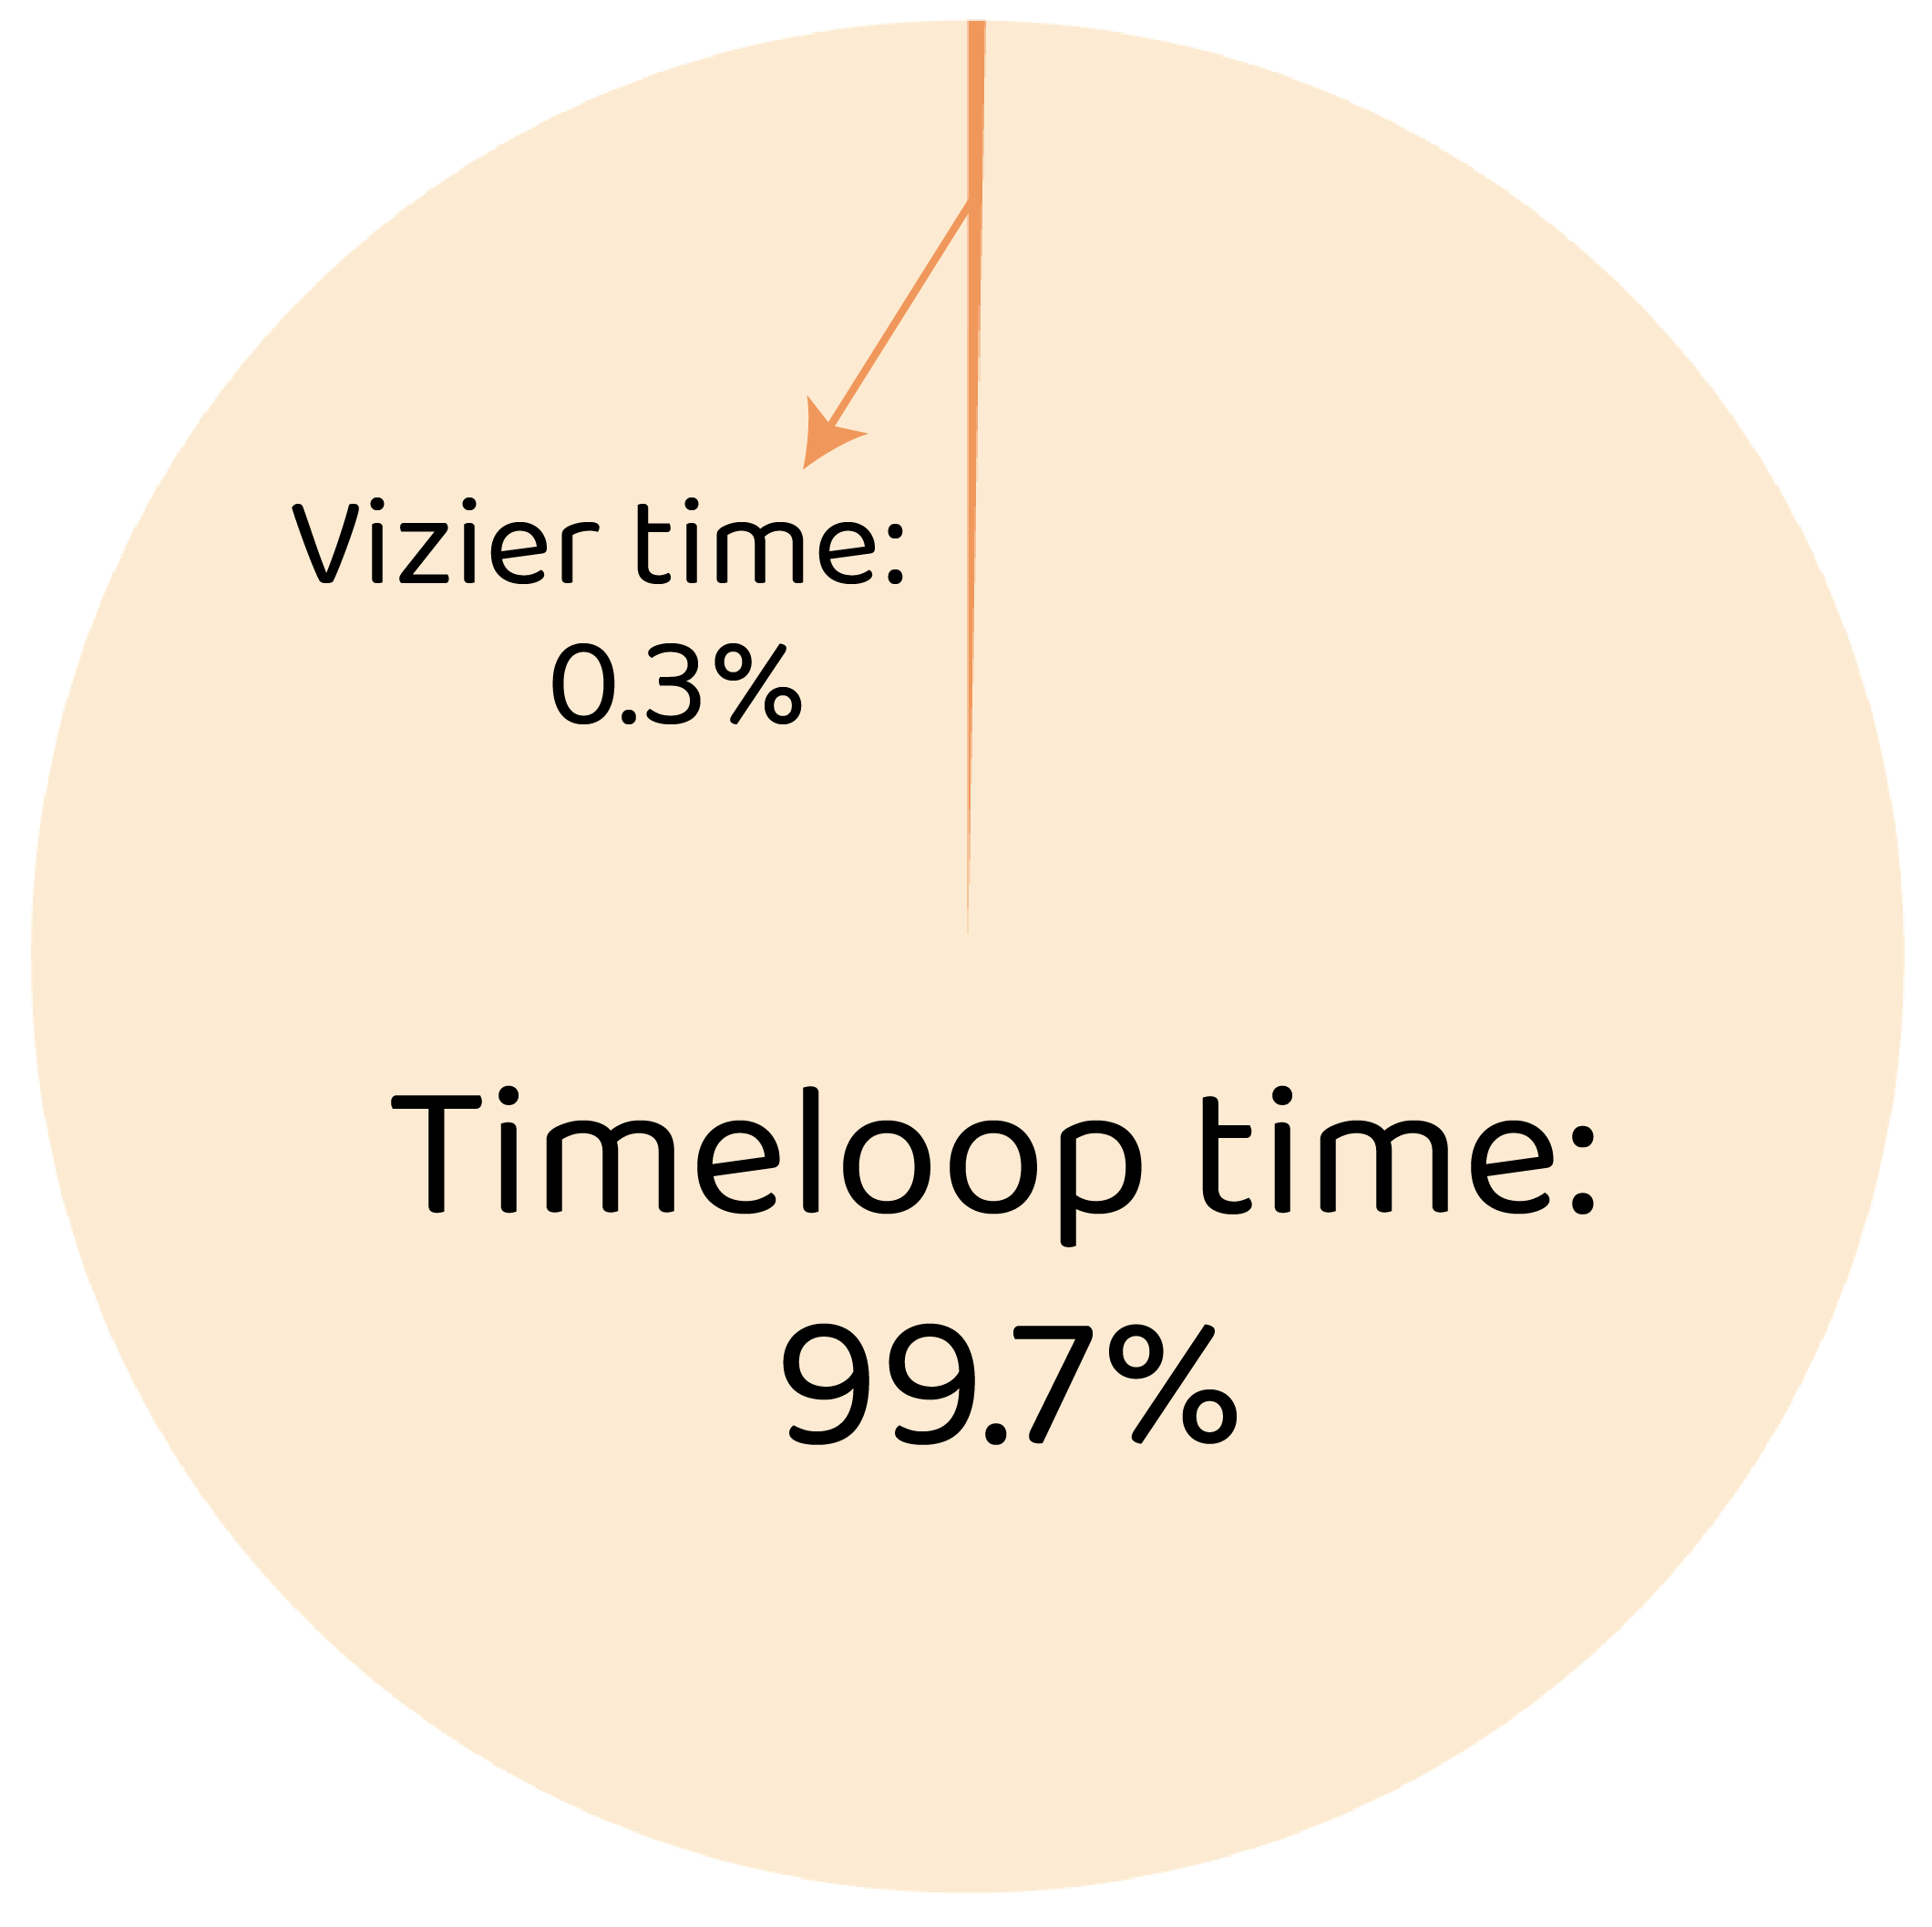
\includegraphics[width=\linewidth]{fig3/timeloop_vs_vizier.png}
% %     \caption{Per-trial wall-clock breakdown.}
% %     \label{fig:timeloop-time}
% %     \vspace{-10pt}
% % \end{wrapfigure}
% % Despite V0's improvements, it inherits the sequential dependence on external tiling tools (e.g., Timeloop) because it lacks a linear expression for non-linear tiling-fusion interactions. As shown in Figure~\ref{fig:timeloop-time}, Timeloop accounts for over 99\% of per-trial latency, creating a prohibitive bottleneck for multi-thousand-trial searches. To resolve this, CHEETAH-V1 internalizes tiling by precomputing Pareto-pruned configurations and encoding them as decision variables. This removes Timeloop from the critical path, collapsing each trial to a single Vizier-proposal and LP-solve step. We start with introducing the preprocessing stage below before presenting the full formulation in Section~\ref{sec::v1}.

% % % The limitations of prior work is still inherited in the V0 formulation due to the difficulty of expressing non-linear relationships as linear constraints. Therefore tiling decisions $(\Tmax_i, \Tmin_i, t_i^k)$ are fixed constants provided by additional software, such as Timeloop. A natural question is whether this sequential dependence also creates a \emph{runtime} bottleneck. Figure~\ref{fig:timeloop-time} confirms that it does: across different models, Timeloop scheduling on average accounts for over 99\% of per-trial wall-clock time, while the Vizier proposal and fusion ILP together consume less than 1\% on average. Because the outer loop requires thousands of trials to converge, the cumulative cost of repeated Timeloop invocations dominates the total search budget. This observation motivates a key design choice in CHEETAH-V1: rather than calling Timeloop online during each trial, we precompute a Pareto-pruned set of tiling configurations once (Section~\ref{sec:pareto}) and encode the tiling selection as decision variables \emph{inside} the LP. This eliminates Timeloop from the per-trial critical path entirely, reducing each trial to a single Vizier-proposal$\,\to\,$LP-solve step.

% % % CHEETAH-V1 captures tiling as a \emph{decision variable} inside the LP, enabling the solver to jointly optimize tiling and fusion. We start with describing our preprocessing stage in Section~\ref{sec:pareto} before presenting the full formulation in Section~\ref{sec::v1}.


% % \paragraph{Pareto Pruning Pre-Pass} The raw tiling search space for a $7$-dimensional convolution loop with $3$ memory levels is $\mathcal O(10^7)$ configurations per operation. We reduce this to a tractable Pareto-optimal subset $\mathcal{C}_i$ for each operation $i$ via a pre-pass for (1) L1 feasibility where configurations whose tiled working set exceeds L1 scratchpad capacity $C_{L1}$ are discarded; (2) Pareto optimality where a configuration $c$ is retained only if no other configuration achieves both lower $\Tmax_i(c)$ \emph{and} smaller working-set size in the Global Buffer.

% % In practice, Pareto pruning reduces $\mathcal O(10^7)$ raw configurations to $|\mathcal{C}_i| \approx 10^2$ to $10^3$ per operation. Timeloop is run once per (operation, configuration) pair, producing the triple $(\Tmin_i(c), \Tmax_i(c), t_i^k(c))$ for each retained configuration $c \in \mathcal{C}_i$. These are precomputed constants---the LP solver makes no Timeloop calls at solve time.

% % \paragraph{Time-invariant Pareto fronts.}
% % A key observation is that the Pareto front shape is invariant to memory time: configurations are ranked by compute cycles and working-set bytes, neither of which depends on bandwidth. Changing bandwidth rescales the DRAM access cost $t_i^k(c)$ uniformly. This means the Pareto-pruned configuration sets can be precomputed \emph{once} and reused across all Vizier trials that share the same compute configuration class, amortizing the expensive Timeloop precomputation.

% % \subsubsection{The Joint CHEETAH-V1 LP Formulation}\label{sec::v1}

% % \paragraph{From fixed constants to decision variables.}
% % In static and V0 formulations, Timeloop selects a single tiling per operation externally and passes the results to the LP as fixed constants $\Tmax_i$, $\Tmin_i$, $t_i^k$. The DRAM savings from pinning tensor $k$ of operation $i$ is then simply $t_i^k \cdot p_{i,o(i)}^k$---a constant times a variable, which is already linear. V1 brings this tiling choice \emph{inside} the LP by introducing \textbf{tiling selection variables} $y_{i,c} \in [0,1]$, one per Pareto-optimal configuration $c \in \mathcal{C}_i$ from the pre-pass, with the constraint $\sum_c y_{i,c} = 1$ (exactly one configuration is selected per operation). The Timeloop-precomputed constants $\Tmax_i(c)$, $\Tmin_i(c)$, $t_i^k(c)$ now become \emph{per-configuration coefficients} indexed by $c$. This means the DRAM savings term becomes $t_i^k(c) \cdot y_{i,c} \cdot p_{\text{assoc}(i,k),\, o(i)}$. This is a product of \emph{two} decision variables, which is bilinear and cannot be handled by a convex programming directly.
 
% % % \paragraph{Linearization via McCormick envelopes.}
% % % We linearize this product exactly via the classical McCormick substitution. Specifically,  we introduce \textbf{auxiliary variables} $w_{i,c,k} := y_{i,c} \cdot p_{\text{assoc}(i,k),\, o(i)}$ that represent the joint effect of selecting tiling $c$ \emph{and} pinning tensor $k$, constrained by:
% % % \begin{equation}
% % % \label{eq:mccormick}
% % % \begin{aligned}
% % %     w_{i,c,k} &\leq y_{i,c}, \qquad
% % %     w_{i,c,k} \leq p_{\text{assoc}(i,k),\, o(i)} \\
% % %     w_{i,c,k} &\geq y_{i,c} + p_{\text{assoc}(i,k),\, o(i)} - 1, \qquad
% % %     w_{i,c,k} \geq 0
% % % \end{aligned}
% % % \end{equation}
% % % Since both factors lie in $[0,1]$, these four constraints force $w_{i,c,k} = y_{i,c} \cdot p$ at any integer vertex, requiring no manually tuned constants. Together, $y_{i,c}$ and $w_{i,c,k}$ account for 1.6M of the 2.08M variables in the \Vone~ LP (Table~\ref{tab:v1_scale}). \todo{change to MoE?}

% % \paragraph{Linearization via McCormick envelopes.}
% % We linearize this product exactly via the classical McCormick substitution \citep{mccormick1976computability}. Specifically, we introduce \textbf{auxiliary variables} $w_{i,c,k} := y_{i,c} \cdot p_{\text{assoc}(i,k),\, o(i)}$ that represent the joint effect of selecting tiling $c$ \emph{and} pinning tensor $k$, constrained by:
% % \begin{equation}
% % \label{eq:mccormick}
% % \begin{aligned}
% %     w_{i,c,k} &\leq y_{i,c}, \qquad
% %     w_{i,c,k} \leq p_{\text{assoc}(i,k),\, o(i)} \\
% %     w_{i,c,k} &\geq y_{i,c} + p_{\text{assoc}(i,k),\, o(i)} - 1, \qquad
% %     w_{i,c,k} \geq 0
% % \end{aligned}
% % \end{equation}
% % Since both factors lie in $[0,1]$, these four constraints force $w_{i,c,k} = y_{i,c} \cdot p$ at any integer vertex, requiring no manually tuned constants. Together, $y_{i,c}$ and $w_{i,c,k}$ constitute the majority of V1's decision variables (Table~\ref{tab:v1_scale}).
 

% % % \paragraph{Full formulation.}
% % % Combining tiling selection, time-indexed placement, rematerialization, and McCormick linearization, the full V1  formulation is:

% % % \begin{equation}
% % % % \label{eq:v1}
% % % \begin{aligned}
% % % \min \quad & \sum_{i \in \mathcal{N}} T_i + \sum_{i \in \mathcal{N}} \sum_{t \in \mathcal{T}} c_i^{\text{remat}} \, r_{i,t} \\[4pt]
% % % \text{s.t.} \quad
% % % & \sum_{c \in \mathcal{C}_i} y_{i,c} = 1 & \forall\, i \in \mathcal{N} \\[3pt]
% % % & T_i \geq \sum_{c \in \mathcal{C}_i} \Tmax_i(c)\, y_{i,c} - \sum_{c \in \mathcal{C}_i} \sum_{k} t_i^k(c)\, w_{i,c,k} & \forall\, i \in \mathcal{N} \\[3pt]
% % % & T_i \geq \sum_{c \in \mathcal{C}_i} \Tmin_i(c)\, y_{i,c} & \forall\, i \in \mathcal{N} \\[3pt]
% % % & w_{i,c,k} \leq y_{i,c} & \forall\, i, c, k \\
% % % & w_{i,c,k} \leq p_{\text{assoc}(i,k),\, o(i)} & \forall\, i, c, k \\
% % % & w_{i,c,k} \geq y_{i,c} + p_{\text{assoc}(i,k),\, o(i)} - 1 & \forall\, i, c, k \\[3pt]
% % % & \sum_{e \in \mathcal{E}} d_e\, p_{e,t} + \sum_{i \in \mathcal{N}} d_i^W\, p_{i,t}^W \leq \CGM & \forall\, t \in \mathcal{T} \\[3pt]
% % % & p_{e,t} \leq p_{e,t-1} + r_{\text{src}(e),\, t} & \forall\, e, t > o(\text{src}(e)) \\
% % % & p_{i,t}^W \leq p_{i,t-1}^W & \forall\, i, t > o(i) \\[3pt]
% % % & r_{i,t} = 0 & \forall\, i, t \leq o(i) \\
% % % & r_{i,t} \leq p_{e,t} & \forall\, e \in \text{in}(i), t > o(i) \\
% % % & r_{i,t} \leq p_{i,t}^W & \forall\, i, t > o(i) \\[3pt]
% % % & T_i, p_{e,t}, p_{i,t}^W, r_{i,t}, w_{i,c,k} \geq 0 &
% % % \end{aligned}
% % % \tag{\textcolor{skyblue}{V1}}\label{eq:v1}
% % % \end{equation}
% % % full formulation below in appendix 
% % % \begin{equation}
% % % \begin{aligned}
% % % \min \quad & \sum_{i \in \mathcal{N}} T_i + \sum_{i \in \mathcal{N}} \sum_{t \in \mathcal{T}} c_i^{\text{remat}} \, r_{i,t} \\[4pt]
% % % \text{s.t.} \quad
% % % & \sum_{c \in \mathcal{C}_i} y_{i,c} = 1 & \forall\, i \in \mathcal{N} \\[3pt]
% % % & T_i \geq \max\!\left(\sum_{c \in \mathcal{C}_i} \Tmin_i(c)\, y_{i,c},\;\; \sum_{c \in \mathcal{C}_i} \Tmax_i(c)\, y_{i,c} - \sum_{c \in \mathcal{C}_i} \sum_{k} t_i^k(c)\, w_{i,c,k}\right) & \forall\, i \in \mathcal{N} \\[3pt]
% % % & w_{i,c,k} \leq y_{i,c}, \quad w_{i,c,k} \leq p_{\text{assoc}(i,k),\, o(i)}, \quad w_{i,c,k} \geq y_{i,c} + p_{\text{assoc}(i,k),\, o(i)} - 1 & \forall\, i, c, k \\[3pt]
% % % & \sum_{e \in \mathcal{E}} d_e\, p_{e,t} + \sum_{i \in \mathcal{N}} d_i^W\, p_{i,t}^W \leq \CGM & \forall\, t \in \mathcal{T} \\[3pt]
% % % & p_{e,t} \leq p_{e,t-1} + r_{\text{src}(e),\, t} & \forall\, e,\, t > o(\text{src}(e)) \\
% % % & p_{i,t}^W \leq p_{i,t-1}^W & \forall\, i,\, t > o(i) \\[3pt]
% % % & r_{i,t} = 0 \;\; \forall\, t \leq o(i); \quad r_{i,t} \leq \min\!\big(p_{e,t},\, p_{i,t}^W\big) \;\; \forall\, e \in \text{in}(i),\, t > o(i) \\[3pt]
% % % & T_i,\, p_{e,t},\, p_{i,t}^W,\, r_{i,t},\, w_{i,c,k} \geq 0 &
% % % \end{aligned}
% % % \tag{\textcolor{skyblue}{V1}}\label{eq:v1}
% % % \end{equation}

% % \paragraph{Variable and constraint digest.}
% % The V1 formulation inherits all the features of the V0 formulation, and additionally captures tiling by introducing selection variables
% % $y_{i,c} \in [0,1]$, constrained by $\sum_c y_{i,c} = 1$, to choose
% % from $|\mathcal{C}_i|$ Pareto-optimal configurations.
% % Each configuration defines compute costs $T_i^{\max}(c)$,
% % $T_i^{\min}(c)$, and per-tensor DRAM savings $t_i^k(c)$.
% % We linearize the resulting bilinear DRAM-savings term exactly via
% % McCormick auxiliary variables $w_{i,c,k}$, which enforce $w_{i,c,k} \;=\; y_{i,c} \cdot p_{\mathrm{assoc}(i,k),\,o(i)}$ at integer vertices without a relaxation gap.

% % Per-operation latency $T_i$ is lower-bounded by the weighted
% % configuration floor $\sum_c T_i^{\min}(c)\, y_{i,c}$ and the weighted
% % off-chip cost $\sum_c T_i^{\max}(c)\, y_{i,c}$ minus achievable savings
% % $\sum_{c,k} t_i^k(c)\, w_{i,c,k}$.
% % This coupling enables the solver to accept sub-optimal local tiling
% % (higher $T_i^{\max}$) if its smaller memory footprint unlocks global
% % fusion gains that outweigh the compute-utilization loss.
% % Capacity and persistence constraints carry over from V0, utilizing
% % edge-indexed placement $p_{e,t}$ to handle multi-fanout nodes.
% % For DeepSeek-V3, the V1 LP scales to approximately $2{,}504{,}019$ variables, $2{,}983{,}450$ constraints, and $6{,}094{,}156$ non-zeros. Table~\ref{tab:v1_scale} provides a representative breakdown, Table~\ref{tab:comparison} summarizes features of each more powerful formulation; full per-model sizes are in Table~\ref{tab:exp1_lp_sizes} and \ref{tab:exp2_cluster_lp_sizes}. 



% % % The V1 formulation extends V0 by making the tiling configuration a decision variable. The selection variables $y_{i,c} \in [0,1]$, with $\sum_c y_{i,c} = 1$, choose among $|\mathcal{C}_i|$ Pareto-optimal tiling configurations precomputed by Timeloop (Section~\ref{sec:pareto}). Each configuration $c$ determines the operation's compute cost $T_i^{\max}(c)$, on-chip floor $T_i^{\min}(c)$, and per-tensor DRAM savings $t_i^k(c)$.
% % % The DRAM savings term $t_i^k(c) \cdot y_{i,c} \cdot p_{\text{assoc}(i,k),\,o(i)}$ 
% % % is bilinear in the tiling selection and placement variables; we linearize it 
% % % via McCormick auxiliary variables $w_{i,c,k}$, constrained by 
% % % $w_{i,c,k} \leq y_{i,c}$, $w_{i,c,k} \leq p_{\text{assoc}(i,k),\,o(i)}$, and 
% % % $w_{i,c,k} \geq y_{i,c} + p_{\text{assoc}(i,k),\,o(i)} - 1$. 
% % % These three inequalities force $w_{i,c,k} = y_{i,c} \cdot p_{\text{assoc}(i,k),\,o(i)}$ 
% % % at any integer-feasible point (\cref{prop:mccormick_exact}), so the LP exactly captures the 
% % % bilinear interaction without introducing any relaxation gap at integer vertices.
% % % The $T_i$ lower bound now takes the maximum of two configuration-dependent terms: the weighted on-chip floor $\sum_c T_i^{\min}(c)\, y_{i,c}$ and the weighted off-chip cost minus achievable savings $\sum_c T_i^{\max}(c)\, y_{i,c} - \sum_{c,k} t_i^k(c)\, w_{i,c,k}$.
% % % This coupling is the core novelty of V1: the solver can accept a tiling with higher $T_i^{\max}(c)$ (lower compute utilization) if its smaller working set enables pinning decisions that reduce total DRAM traffic by more than the utilization loss.
% % % All remaining constraints---memory capacity, persistence, and rematerialization---carry over from V0 with edge-indexed placement variables $p_{e,t}$ replacing per-tensor $p_{i,t}^k$ to correctly handle skip connections and multi-fanout nodes. For our largest workload, DeepSeek-V3 ($L \approx 6{,}300$ operations), the V1 LP contains approximately 2.5M variables, 3.0M constraints, and 6.1M nonzeros. Table~\ref{tab:v1_scale} provides a representative breakdown; full per-model sizes are in Table~\ref{tab:v1_scale}. 
% % % \paragraph{Key constraint interactions.}
% % % The execution-time constraints (lines 2--3: the upper and lower bounds for $T_i$) capture the central trade-off that is unique to \Vone: the LP must commit to a tiling configuration $c$ (via $y_{i,c}$) that sets both the baseline compute cost $\Tmax_i(c)$ and the achievable DRAM savings $t_i^k(c)$. A configuration with smaller tiles may have higher $\Tmax_i(c)$ (lower compute utilization) but smaller working sets, enabling more aggressive pinning. The LP balances these trade-offs simultaneously---precisely the cross-stage interaction that the sequential pipeline cannot discover.
 
% % % The edge-indexed persistence constraint (line 8: $p_{e,t} \leq p_{e,t-1} + r_{\text{src}(e),\, t}$) and the memory capacity constraint (line 7: lower bound on $\CGM$) are inherited from \Vzero, which introduced per-edge placement variables $p_{e,t}$ to correctly model skip connections. \Vone~ extends this by coupling edge sizes to the tiling selection---since different configurations $c$ produce different activation working sets, the LP can now jointly reason about how tiling choices affect memory pressure across skip connections.


% % \begin{figure}[ht!]
% % \begin{minipage}[t]{0.48\textwidth}
% % \vspace{0pt}
% % \centering
% % \captionof{table}{V1 variable and constraint counts
% % (representative, DeepSeek-V3).}
% % \label{tab:v1_scale}
% % \footnotesize
% % \begin{tabular}{@{}ll@{}}
% % \toprule
% % \textbf{Variable} & \textbf{Role} \\
% % \midrule
% % $T_i$       & Per-operation execution time \\
% % $y_{i,c}$   & Tiling config selection ($|\mathcal{C}_i|$ options) \\
% % $p_{e,t}$   & Edge-indexed activation placement \\
% % $p_{i,t}^W$ & Weight placement \\
% % $r_{i,t}$   & Rematerialization indicator \\
% % $w_{i,c,k}$ & McCormick auxiliaries ($y_{i,c} \cdot p$) \\
% % % \midrule
% % % \multicolumn{2}{@{}l}{\textbf{DeepSeek-V3 totals}
% % %                        ($L \approx 6{,}300$)} \\
% % % \midrule
% % % Variables   & $2{,}504{,}019$ \\
% % % Constraints & $2{,}983{,}450$ \\
% % % Nonzeros    & $6{,}094{,}156$ \\
% % \bottomrule
% % \end{tabular}
% % \end{minipage}%
% % \hspace{0.02\textwidth}%
% % \begin{minipage}[t]{0.48\textwidth}
% % \vspace{0pt}
% % \centering
% % \captionof{table}{Comparison of static, V0, and V1 formulations.}
% % \label{tab:comparison}
% % \footnotesize
% % \begin{tabular}{@{}lccc@{}}
% % \toprule
% % \textbf{Property} & \textbf{Static} & \textbf{V0} & \textbf{V1} \\
% % \midrule
% % Joint tiling + fusion    & $\times$ & $\times$   & \checkmark \\
% % Time-indexed placement   & $\times$ & \checkmark & \checkmark \\
% % Rematerialization        & $\times$ & \checkmark & \checkmark \\
% % Relaxed skip connections & $\times$ & Partial    & \checkmark \\
% % \bottomrule
% % \end{tabular}

% % \medskip
% % \raggedright
% % \footnotesize
% % % \textbf{Comparison across formulations.}
% % % Table~\ref{tab:comparison} summarizes the progression from the
% % % static formulation through V0 to V1.
% % \end{minipage}
% % \end{figure}


% % % \begin{table}[ht!]
% % % \centering
% % % \caption{V1 variable and constraint counts (representative, DeepSeek-V3).}
% % % \label{tab:v1_scale}
% % % \small
% % % \begin{tabular}{lrl}
% % % \toprule
% % % \textbf{Variable} & \textbf{Role} \\
% % % \midrule
% % % $T_i$ & Per-operation execution time \\
% % % $y_{i,c}$ & Tiling configuration selection ($|\mathcal{C}_i|$ options per op) \\
% % % $p_{e,t}$ & Edge-indexed activation placement \\
% % % $p_{i,t}^W$ & Weight placement \\
% % % $r_{i,t}$ & Rematerialization indicator \\
% % % $w_{i,c,k}$ & McCormick auxiliaries ($y_{i,c} \cdot p$) \\
% % % \midrule
% % % \multicolumn{2}{l}{\textbf{DeepSeek-V3 totals} ($L \approx 6{,}300$)} \\
% % % \midrule
% % % Variables & 2,504,019 \\
% % % Constraints & 2,983,450 \\
% % % Nonzeros & 6,094,156 \\
% % % \bottomrule
% % % \end{tabular}
% % % \end{table}
% % % \paragraph{Comparison across formulations.}
% % % Table~\ref{tab:comparison} summarizes the progression from static through V0 to V1.
% % % \begin{table}[ht!]
% % % \centering
% % % \caption{Comparison of static, V0, and V1 formulations.}
% % % \label{tab:comparison}
% % % \small
% % % \begin{tabular}{lccc}
% % % \toprule
% % % \textbf{Property} & \textbf{static} & \textbf{V0} & \textbf{V1} \\
% % % \midrule
% % % Joint tiling + fusion & \texttimes & \texttimes & \checkmark \\
% % % Time-indexed placement & \texttimes & \checkmark & \checkmark \\
% % % Rematerialization & \texttimes & \checkmark & \checkmark \\
% % % Relaxed skip connections & \texttimes & Partial & \checkmark \\
% % % % Config-dependent DRAM savings & \texttimes & \texttimes & \checkmark \\ 
% % % % Bilinear linearization & --- & --- & McCormick \\
% % % \bottomrule
% % % \end{tabular}
% % % \end{table}

% % % \paragraph{Structural invariance for efficient LLM integration.}
% % % A practical advantage of both our LP formulations is that the constraint matrix sparsity pattern is invariant across hardware configurations---only the numerical coefficients change. This means:
% % % \begin{itemize}
% % %     \item The LP solver's preconditioner can be designed once per neural network model and reused across all Vizier trials.
% % %     \item An LLM-Architect can reason about constraint structure (which constraints are binding, which variables are fractional) without needing to understand the full LP.
% % %     \item Warm-starting from a previous trial's LP solution is straightforward since the variable indexing is stable.
% % % \end{itemize}

% % \subsection{Strategic Intelligence: LLM-Guided Outer Search}
% % \label{sec:llm_outer}
% % We use Google Vizier as a black-box Bayesian optimizer to propose hardware configurations. While effective, vanilla Vizier treats search as pure function optimization, often requiring thousands of iterations to identify suboptimal regions without leveraging structural hardware-workload knowledge. To address this, we introduce an LLM-guided outer-loop controller based on SkyDiscovery that reasons about co-design decisions. By learning from a causal ledger of past trials and Lagrangian dual signals from the LP solver, the LLM proposes meaningful, constrained search-space candidates. This integration is enabled by the CHEETAH-V1 formulation, which removes the Timeloop bottleneck to reduce trial times from days to hours.The LLM-Architect reduces wasted trials by intelligently steering Vizier’s search without altering the inner solver or its optimality certificates. In this hybrid loop, the LLM determines global architectural regions, Vizier performs local Bayesian optimization within those patches, and the large-scale V1 LP solver evaluates each concrete candidate. The LLM-Architect loop proceeds as follows: 
% % % We use Vizier as a black-box Bayesian optimizer to propose candidate hardware configurations. While effective, Vizier search strategies (LCS, UCB, etc) requires thousands of iterations explore and learn which regions are suboptimal and treats the search as a pure function optimization problem without leveraging structural knowledge about hardware-workload interactions.
% % % We leverage an LLM-guided outer-loop controller that learns from logs of thousands of past co-design trials to propose meaningful search-space candidates for Vizier. This is a SkyDiscovery based outer LLM layer which reasons about hardware-software co-design decisions and learns from a causal ledger of constantly updated logs across trials, as well as feed-back signal such as dual variables through the LP solve. This is possible for CHEETAH-V1 LP formulation, since it removes the Timeloop-in-the-loop constraint, thus reducing the co-design problem from days to hours, and permitting the LLM outer loop. 

% % % The LLM-Architect does not change the inner solver, and retains all the optimal certificates of the V1 LP formulation, but intelligently changes where the Vizier outer hardware optimizer searches to reduce wasted trials. The LLM proposes global decisions to determine constrained regions of the hardware search space; Vizier then performs local Bayesian optimization inside those regions; which then passes downstream into a large scale LP solver for the V1 formulation to evaluate each concrete candidate. The LLM-Architect loop proceeds as follows:

% % \begin{enumerate}[leftmargin=1.6em, itemsep=4pt]

% % \item \textbf{Extraction.}
% % Deterministic scripts summarize recent trials into a \emph{Causal
% % Ledger}. Each record includes hardware parameters, validity, Perf/TDP,
% % LP cycles, capacity duals/slacks, bandwidth sensitivity, MFU, memory
% % utilization, roofline gap, failure class, and LP solver metrics.

% % \item \textbf{Context building.}
% % The last $N$ trials and the Causal Ledger are compressed into a compact
% % JSON context for the Architect. The context emphasizes empirical
% % feasibility, observed invalid regions, best known valid designs, and
% % physical audit signals.

% % \item \textbf{Architect.}
% % The online Architect, implemented as Qwen2.5-7B-Instruct with a LoRA
% % adapter trained on past trial logs, diagnoses the dominant bottleneck
% % and emits a campaign patch. The patch constrains macro-architectural
% % search decisions such as Global Memory, DRAM bandwidth, total MACs,
% % systolic shape, PE grid, and batch size. A larger teacher model,
% % DeepSeek-V3.2, was used offline to generate or critique campaign labels
% % but is not in the live loop.

% % \item \textbf{Campaign validation.}
% % A deterministic validator clips or rejects the LLM patch to enforce
% % legal hardware ranges, TDP and area limits, MAC caps, CGM feasibility
% % floors, compute/bandwidth coupling, and roofline constraints. This
% % prevents the LLM from proposing physically implausible regions such as
% % maximum-MAC/minimum-bandwidth designs.

% % \item \textbf{Local optimization.}
% % Vizier is initialized inside the validated patch and warm-started with
% % prior trials that lie in the same region. Vizier then samples concrete
% % hardware candidates within the approved campaign. The LLM therefore
% % chooses the high-level architectural neighbourhood, while Vizier
% % performs local adaptive optimization.

% % \item \textbf{Unified V1 evaluation.}
% % The large-scale LP solver evaluates each candidate by solving the V1
% % joint tiling-fusion-placement LP using saved Pareto $\mathcal{C}$-sets.
% % It returns the objective, cycles, selected tiling configurations,
% % placement/rematerialization decisions, dual/slack summaries, and
% % solver-quality diagnostics.

% % \item \textbf{Roofline audit.}
% % A deterministic Roofline Auditor checks whether the predicted latency
% % is physically plausible. For each candidate we compute
% % \begin{align}
% %     t_{\text{compute}} &=
% %         \frac{\text{useful FLOPs}}{\text{peak FLOPs/s}},
% %     \qquad
% %     t_{\text{memory}}  =
% %         \frac{\text{post-placement DRAM bytes}}{\text{peak bandwidth}},
% %     \nonumber\\
% %     t_{\text{ideal}}   &=
% %         \max\!\left(t_{\text{compute}},\, t_{\text{memory}}\right).
% %     \label{eq:roofline_audit}
% % \end{align}
% % A candidate is rejected if the solver-reported latency falls below this
% % lower bound, or if MFU or memory utilization exceeds 1.0 within
% % tolerance.

% % \item \textbf{Ledger update.}
% % The loop records the campaign hypothesis, intervention, observed
% % invalid-rate change, MFU change, roofline validity, and best Perf/TDP
% % change. The ledger also records forbidden regions when a campaign
% % produces excessive invalid trials.

% % \end{enumerate}

% % \noindent The Architect receives workload summaries, invalid-rate
% % history, MFU, roofline signals, prior valid regions, normalized LP duals,
% % and bandwidth sensitivities. The system starts from a safe empirically
% % valid patch and permits duals only to make bounded edits, such as raising
% % the CGM floor, increasing bandwidth, reducing MAC count, or changing
% % systolic shapes. The validator rejects any dual-guided patch that
% % excludes known high-performing valid regions or predicts a substantially
% % worse feasible rate. This provides controlled architectural feedback in
% % addition to prompt input.


% % % \todo{Expand this section once the LLM+RL experimental protocol is finalized. Key questions to address: (1) Which LLM is used and how is it prompted? (2) How are LLM proposals integrated with Vizier's Bayesian model? (3) What is the sample efficiency improvement over pure Vizier?}





% % edit for page limit 

% \section{Methodology}
% \label{sec:methods}

% We present the CHEETAH (\acroletter{C}o-designed \acroletter{H}ardware \acroletter{E}xploration via \acroletter{E}fficient \acroletter{T}hroughput and \acroletter{H}ybrid-search) framework in three parts: Section~\ref{sec:v0} introduces CHEETAH-V0, which extends the static fusion ILP with time-indexed placement and rematerialization. Section~\ref{sec:v1} presents CHEETAH-V1, which jointly optimizes tiling and fusion via McCormick linearization. Section~\ref{sec:llm_outer} describes the LLM-Architect outer loop.


% % \subsection{\Vzero~: Multi-Period Placement with Rematerialization}
% \subsection{CHEETAH-V0: Multi-Period Placement with Rematerialization}
% \label{sec:v0}

% Our first extension models the neural network's execution as a sequence of $T$ discrete timesteps (one per operation in execution order). This decides at which time, which tensor is pinned, evicted, or recomputed to optimally minimize cycle counts. The key features are:

% \paragraph{Time-indexed placement.}
% Instead of a single binary $p_i^k$ per tensor, we introduce $p_{i,t}^k \in [0,1]$ for each tensor $k$ of layer $i$ at each timestep $t$. A tensor can be pinned at timestep $t=5$, and evicted at $t=10$. This models a dynamic memory manager within a single inference pass.

% \paragraph{Rematerialization.}
% Rather than always paying DRAM bandwidth to reload an evicted tensor, we introduce variables $r_{i,t} \in [0,1]$ indicating that layer $i$ is recomputed at timestep $t$ to restore its output to the Global Buffer. This is particularly valuable for models such as EfficientNet, where depthwise convolutions account for only ${\sim}5\%$ of total FLOPs but produce large activation tensors. Recomputing a depthwise layer to avoid re-reading 6\,MiB from DRAM at 256\,GB/s can be faster than the DRAM reload itself.

% \paragraph{Relaxed skip-connection handling.}
% We lift the limitation of our baseline original ILP, which restricts activation pinning to consecutively-executed operations and limits multi-fanout nodes so that at most one consumer benefits from on-chip data. CHEETAH-V0 uses edge-indexed placement variables $p_{e,t}$ for each edge $e \in \mathcal{E}$ of the dataflow graph, correctly modeling the case where one consumer of a skip connection benefits from on-chip data while another does not.

% The CHEETAH-V0 LP formulation is:
% \begin{equation}
% % \label{eq:v0}
% \begin{aligned}
% \min \quad & \sum_{i \in \mathcal{N}} T_i + \sum_{i \in \mathcal{N}} \sum_{t \in \mathcal{T}} c_i^{\text{remat}} \, r_{i,t} \\
% \text{s.t.} \quad
% & T_i \geq \Tmax_i - \sum_{k \in \{I,O,W\}} t_i^k \cdot p_{i,o(i)}^k & \forall\, i \in \mathcal{N} \\
% & T_i \geq \Tmin_i & \forall\, i \in \mathcal{N} \\
% & \sum_{i \in \mathcal{N}} \sum_{k} d_i^k \, p_{i,t}^k \leq \CGM & \forall\, t \in \mathcal{T} \\
% & p_{i,t}^k \leq p_{i,t-1}^k + r_{i,t} & \forall\, i, t, k \in \{I,O\} \\
% & p_{i,t}^W \leq p_{i,t-1}^W & \forall\, i, t \\
% & r_{i,t} = 0 & \forall\, i, t \leq o(i) \\
% & 0 \leq p_{i,t}^k, r_{i,t} \leq 1 &
% \end{aligned}
% \tag{V0}\label{eq:v0}
% \end{equation}


% where $o(i)$ is the execution order of operation $i$, $d_i^k$ is the byte size of tensor $k$ for layer $i$, and $c_i^{\text{remat}}$ is the recomputation cost.

% \paragraph{Variable and constraint digest.}
% The V0 objective minimizes the sum of execution times $\sum_i T_i$ and
% rematerialization costs $c_i^{\text{remat}}\, r_{i,t}$.
% Per-operation latency $T_i$ is lower-bounded by the physical on-chip
% floor $T_i^{\min}$ and the off-chip time $T_i^{\max}$ adjusted for DRAM
% savings $t_i^k \cdot p_{i,o(i)}^k$ from pinned tensors.
% Placement variables $p_{i,t}^k \in [0,1]$ track Global Memory residency
% for inputs, outputs, and weights at each timestep, subject to a global
% capacity constraint $C_{\text{GM}}$. Persistence is governed by $p_{i,t}^k \;\leq\; p_{i,t-1}^k + r_{i,t},$ enforcing that activations are either resident from the previous timestep
% or recomputed; weight tensors satisfy the stricter monotone constraint
% $p_{i,t}^W \leq p_{i,t-1}^W$, as weights cannot be rematerialized.
% Rematerialization $r_{i,t}$ is only permitted post-execution
% ($t > o(i)$) and requires on-chip availability of both inputs and
% weights.
% For DeepSeek-V3 ($L \approx 6{,}300$), this formulation yields a
% large-scale program with approximately 3.3M variables and 3.7M
% constraints.


% % \subsection{\textcolor{skyblue}{V1}: Joint Tiling and Fusion via McCormick Linearization}
% \subsection{CHEETAH-V1: Joint Tiling and Fusion via McCormick Linearization}
% \label{sec:v1}

% \begin{wrapfigure}{r}{0.2\linewidth}
%     \vspace{-12pt}
%     \centering
%     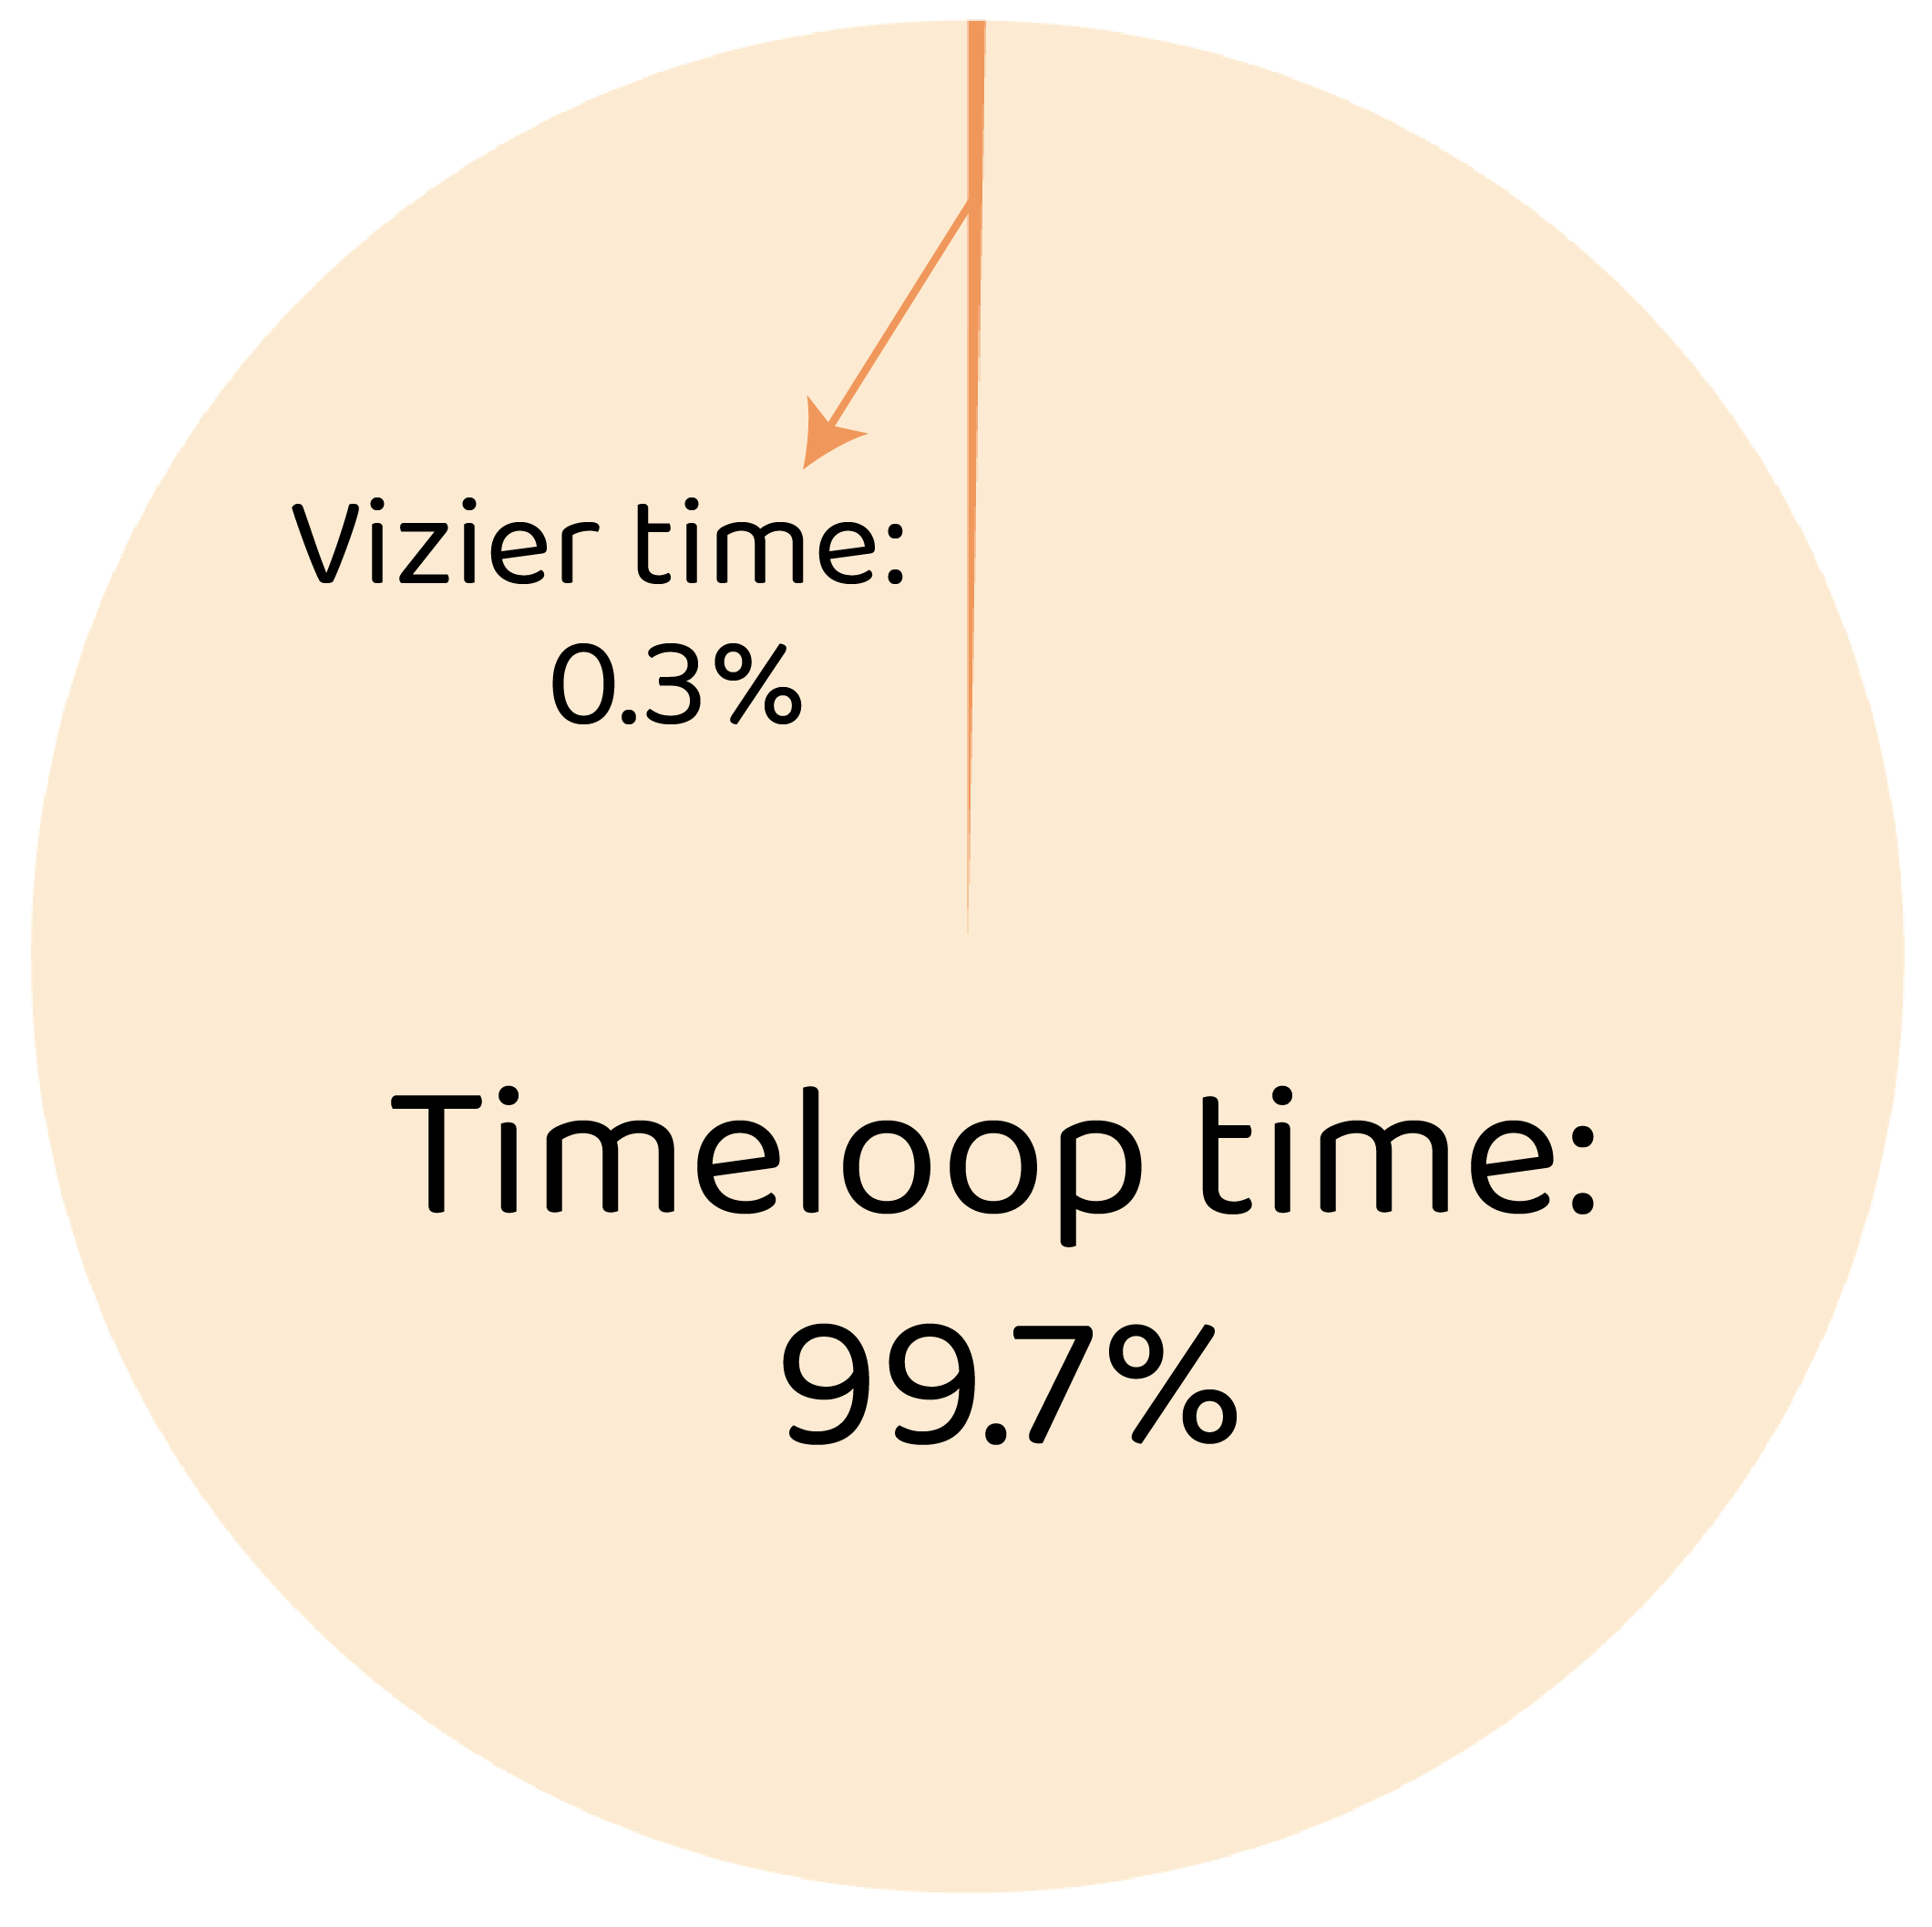
\includegraphics[width=\linewidth]{fig3/timeloop_vs_vizier.png}
%     \caption{Per-trial wall-clock breakdown.}
%     \label{fig:timeloop-time}
%     \vspace{-10pt}
% \end{wrapfigure}
% Despite V0's improvements, it inherits the sequential dependence on external tiling tools (e.g., Timeloop) because it lacks a linear expression for non-linear tiling-fusion interactions. As shown in Figure~\ref{fig:timeloop-time}, Timeloop accounts for over 99\% of per-trial latency, creating a prohibitive bottleneck for multi-thousand-trial searches. To resolve this, CHEETAH-V1 internalizes tiling by precomputing Pareto-pruned configurations and encoding them as decision variables. This removes Timeloop from the critical path, collapsing each trial to a single Vizier-proposal and LP-solve step. We start with introducing the preprocessing stage below before presenting the full formulation in Section~\ref{sec::v1}.

% % The limitations of prior work is still inherited in the V0 formulation due to the difficulty of expressing non-linear relationships as linear constraints. Therefore tiling decisions $(\Tmax_i, \Tmin_i, t_i^k)$ are fixed constants provided by additional software, such as Timeloop. A natural question is whether this sequential dependence also creates a \emph{runtime} bottleneck. Figure~\ref{fig:timeloop-time} confirms that it does: across different models, Timeloop scheduling on average accounts for over 99\% of per-trial wall-clock time, while the Vizier proposal and fusion ILP together consume less than 1\% on average. Because the outer loop requires thousands of trials to converge, the cumulative cost of repeated Timeloop invocations dominates the total search budget. This observation motivates a key design choice in CHEETAH-V1: rather than calling Timeloop online during each trial, we precompute a Pareto-pruned set of tiling configurations once (Section~\ref{sec:pareto}) and encode the tiling selection as decision variables \emph{inside} the LP. This eliminates Timeloop from the per-trial critical path entirely, reducing each trial to a single Vizier-proposal$\,\to\,$LP-solve step.

% % CHEETAH-V1 captures tiling as a \emph{decision variable} inside the LP, enabling the solver to jointly optimize tiling and fusion. We start with describing our preprocessing stage in Section~\ref{sec:pareto} before presenting the full formulation in Section~\ref{sec::v1}.


% \paragraph{Pareto Pruning Pre-Pass.} The raw tiling search space for a $7$-dimensional convolution loop with $3$ memory levels is $\mathcal O(10^7)$ configurations per operation. We reduce this to a tractable Pareto-optimal subset $\mathcal{C}_i$ for each operation $i$ via a pre-pass for (1) L1 feasibility where configurations whose tiled working set exceeds L1 scratchpad capacity $C_{L1}$ are discarded; (2) Pareto optimality where a configuration $c$ is retained only if no other configuration achieves both lower $\Tmax_i(c)$ \emph{and} smaller working-set size in the Global Buffer.

% In practice, Pareto pruning reduces $\mathcal O(10^7)$ raw configurations to $|\mathcal{C}_i| \approx 10^2$ to $10^3$ per operation. Timeloop is run once per (operation, configuration) pair, producing the triple $(\Tmin_i(c), \Tmax_i(c), t_i^k(c))$ for each retained configuration $c \in \mathcal{C}_i$. These are precomputed constants---the LP solver makes no Timeloop calls at solve time.

% \paragraph{Time-invariant Pareto fronts.}
% A key observation is that the Pareto front shape is invariant to memory time: configurations are ranked by compute cycles and working-set bytes, neither of which depends on bandwidth. Changing bandwidth rescales the DRAM access cost $t_i^k(c)$ uniformly. This means the Pareto-pruned configuration sets can be precomputed \emph{once} and reused across all Vizier trials that share the same compute configuration class, amortizing the expensive Timeloop precomputation.

% % \subsubsection{The Joint CHEETAH-V1 LP Formulation}\label{sec::v1}

% \paragraph{From fixed constants to decision variables.}
% In static and V0 formulations, Timeloop selects a single tiling per operation externally and passes the results to the LP as fixed constants $\Tmax_i$, $\Tmin_i$, $t_i^k$. The DRAM savings from pinning tensor $k$ of operation $i$ is then simply $t_i^k \cdot p_{i,o(i)}^k$---a constant times a variable, which is already linear. V1 brings this tiling choice \emph{inside} the LP by introducing \textbf{tiling selection variables} $y_{i,c} \in [0,1]$, one per Pareto-optimal configuration $c \in \mathcal{C}_i$ from the pre-pass, with the constraint $\sum_c y_{i,c} = 1$ (exactly one configuration is selected per operation). The Timeloop-precomputed constants $\Tmax_i(c)$, $\Tmin_i(c)$, $t_i^k(c)$ now become \emph{per-configuration coefficients} indexed by $c$. This means the DRAM savings term becomes $t_i^k(c) \cdot y_{i,c} \cdot p_{\text{assoc}(i,k),\, o(i)}$. This is a product of \emph{two} decision variables, which is bilinear and cannot be handled by a convex programming directly.
 
% % \paragraph{Linearization via McCormick envelopes.}
% % We linearize this product exactly via the classical McCormick substitution. Specifically,  we introduce \textbf{auxiliary variables} $w_{i,c,k} := y_{i,c} \cdot p_{\text{assoc}(i,k),\, o(i)}$ that represent the joint effect of selecting tiling $c$ \emph{and} pinning tensor $k$, constrained by:
% % \begin{equation}
% % \label{eq:mccormick}
% % \begin{aligned}
% %     w_{i,c,k} &\leq y_{i,c}, \qquad
% %     w_{i,c,k} \leq p_{\text{assoc}(i,k),\, o(i)} \\
% %     w_{i,c,k} &\geq y_{i,c} + p_{\text{assoc}(i,k),\, o(i)} - 1, \qquad
% %     w_{i,c,k} \geq 0
% % \end{aligned}
% % \end{equation}
% % Since both factors lie in $[0,1]$, these four constraints force $w_{i,c,k} = y_{i,c} \cdot p$ at any integer vertex, requiring no manually tuned constants. Together, $y_{i,c}$ and $w_{i,c,k}$ account for 1.6M of the 2.08M variables in the \Vone~ LP (Table~\ref{tab:v1_scale}). \todo{change to MoE?}

% \paragraph{Linearization via McCormick envelopes.}
% We linearize this product exactly via the classical McCormick substitution \citep{mccormick1976computability}. Specifically, we introduce \textbf{auxiliary variables} $w_{i,c,k} := y_{i,c} \cdot p_{\text{assoc}(i,k),\, o(i)}$ that represent the joint effect of selecting tiling $c$ \emph{and} pinning tensor $k$, constrained by:
% \begin{equation}
% \label{eq:mccormick}
% \begin{aligned}
%     w_{i,c,k} &\leq y_{i,c}, \qquad
%     w_{i,c,k} \leq p_{\text{assoc}(i,k),\, o(i)} \\
%     w_{i,c,k} &\geq y_{i,c} + p_{\text{assoc}(i,k),\, o(i)} - 1, \qquad
%     w_{i,c,k} \geq 0
% \end{aligned}
% \end{equation}
% Since both factors lie in $[0,1]$, these four constraints force $w_{i,c,k} = y_{i,c} \cdot p$ at any integer vertex, requiring no manually tuned constants. Together, $y_{i,c}$ and $w_{i,c,k}$ constitute the majority of V1's decision variables (Table~\ref{tab:v1_scale}).

% \paragraph{The Joint CHEETAH-V1 LP Formulation.}
% Combining tiling selection, time-indexed placement, rematerialization, and McCormick linearization, the full V1 formulation is:
% \begin{equation}
% \begin{aligned}
% \min \quad & \sum_{i \in \mathcal{N}} T_i + \sum_{i \in \mathcal{N}} \sum_{t \in \mathcal{T}} c_i^{\text{remat}} \, r_{i,t} \\[4pt]
% \text{s.t.} \quad
% & \sum_{c \in \mathcal{C}_i} y_{i,c} = 1 & \forall\, i \in \mathcal{N} \\[3pt]
% & T_i \geq \max\!\left(\sum_{c \in \mathcal{C}_i} \Tmin_i(c)\, y_{i,c},\;\; \sum_{c \in \mathcal{C}_i} \Tmax_i(c)\, y_{i,c} - \sum_{c \in \mathcal{C}_i} \sum_{k} t_i^k(c)\, w_{i,c,k}\right) & \forall\, i \in \mathcal{N} \\[3pt]
% & w_{i,c,k} \leq y_{i,c}, \quad w_{i,c,k} \leq p_{\text{assoc}(i,k),\, o(i)}, \quad w_{i,c,k} \geq y_{i,c} + p_{\text{assoc}(i,k),\, o(i)} - 1 & \forall\, i, c, k \\[3pt]
% & \sum_{e \in \mathcal{E}} d_e\, p_{e,t} + \sum_{i \in \mathcal{N}} d_i^W\, p_{i,t}^W \leq \CGM & \forall\, t \in \mathcal{T} \\[3pt]
% & p_{e,t} \leq p_{e,t-1} + r_{\text{src}(e),\, t} & \forall\, e,\, t > o(\text{src}(e)) \\
% & p_{i,t}^W \leq p_{i,t-1}^W & \forall\, i,\, t > o(i) \\[3pt]
% & r_{i,t} = 0 \;\; \forall\, t \leq o(i); \quad r_{i,t} \leq \min\!\big(p_{e,t},\, p_{i,t}^W\big) \;\; \forall\, e \in \text{in}(i),\, t > o(i) \\[3pt]
% & T_i,\, p_{e,t},\, p_{i,t}^W,\, r_{i,t},\, w_{i,c,k} \geq 0 &
% \end{aligned}
% \tag{V1}\label{eq:v1}
% \end{equation}

% \paragraph{Variable and constraint digest.}
% The V1 formulation inherits all the features of the V0 formulation, and additionally captures tiling by introducing selection variables
% $y_{i,c} \in [0,1]$, constrained by $\sum_c y_{i,c} = 1$, to choose
% from $|\mathcal{C}_i|$ Pareto-optimal configurations.
% Each configuration defines compute costs $T_i^{\max}(c)$,
% $T_i^{\min}(c)$, and per-tensor DRAM savings $t_i^k(c)$.
% We linearize the resulting bilinear DRAM-savings term exactly via
% McCormick auxiliary variables $w_{i,c,k}$, which enforce $w_{i,c,k} \;=\; y_{i,c} \cdot p_{\mathrm{assoc}(i,k),\,o(i)}$ at integer vertices without a relaxation gap.

% Per-operation latency $T_i$ is lower-bounded by the weighted
% configuration floor $\sum_c T_i^{\min}(c)\, y_{i,c}$ and the weighted
% off-chip cost $\sum_c T_i^{\max}(c)\, y_{i,c}$ minus achievable savings
% $\sum_{c,k} t_i^k(c)\, w_{i,c,k}$.
% This coupling enables the solver to accept sub-optimal local tiling
% (higher $T_i^{\max}$) if its smaller memory footprint unlocks global
% fusion gains that outweigh the compute-utilization loss.
% Capacity and persistence constraints carry over from V0, utilizing
% edge-indexed placement $p_{e,t}$ to handle multi-fanout nodes.
% For DeepSeek-V3, the V1 LP scales to approximately 2.5M variables,
% 3.0M constraints and 6.1M nonzeros. Table~\ref{tab:v1_scale} provides a representative breakdown, Table~\ref{tab:comparison} summarizes features of each formulation; full per-model sizes are in Table~\ref{tab:exp1_lp_sizes} and \ref{tab:exp2_cluster_lp_sizes}. 



% % The V1 formulation extends V0 by making the tiling configuration a decision variable. The selection variables $y_{i,c} \in [0,1]$, with $\sum_c y_{i,c} = 1$, choose among $|\mathcal{C}_i|$ Pareto-optimal tiling configurations precomputed by Timeloop (Section~\ref{sec:pareto}). Each configuration $c$ determines the operation's compute cost $T_i^{\max}(c)$, on-chip floor $T_i^{\min}(c)$, and per-tensor DRAM savings $t_i^k(c)$.
% % The DRAM savings term $t_i^k(c) \cdot y_{i,c} \cdot p_{\text{assoc}(i,k),\,o(i)}$ 
% % is bilinear in the tiling selection and placement variables; we linearize it 
% % via McCormick auxiliary variables $w_{i,c,k}$, constrained by 
% % $w_{i,c,k} \leq y_{i,c}$, $w_{i,c,k} \leq p_{\text{assoc}(i,k),\,o(i)}$, and 
% % $w_{i,c,k} \geq y_{i,c} + p_{\text{assoc}(i,k),\,o(i)} - 1$. 
% % These three inequalities force $w_{i,c,k} = y_{i,c} \cdot p_{\text{assoc}(i,k),\,o(i)}$ 
% % at any integer-feasible point (\cref{prop:mccormick_exact}), so the LP exactly captures the 
% % bilinear interaction without introducing any relaxation gap at integer vertices.
% % The $T_i$ lower bound now takes the maximum of two configuration-dependent terms: the weighted on-chip floor $\sum_c T_i^{\min}(c)\, y_{i,c}$ and the weighted off-chip cost minus achievable savings $\sum_c T_i^{\max}(c)\, y_{i,c} - \sum_{c,k} t_i^k(c)\, w_{i,c,k}$.
% % This coupling is the core novelty of V1: the solver can accept a tiling with higher $T_i^{\max}(c)$ (lower compute utilization) if its smaller working set enables pinning decisions that reduce total DRAM traffic by more than the utilization loss.
% % All remaining constraints---memory capacity, persistence, and rematerialization---carry over from V0 with edge-indexed placement variables $p_{e,t}$ replacing per-tensor $p_{i,t}^k$ to correctly handle skip connections and multi-fanout nodes. For our largest workload, DeepSeek-V3 ($L \approx 6{,}300$ operations), the V1 LP contains approximately 2.5M variables, 3.0M constraints, and 6.1M nonzeros. Table~\ref{tab:v1_scale} provides a representative breakdown; full per-model sizes are in Table~\ref{tab:v1_scale}. 
% % \paragraph{Key constraint interactions.}
% % The execution-time constraints (lines 2--3: the upper and lower bounds for $T_i$) capture the central trade-off that is unique to \Vone: the LP must commit to a tiling configuration $c$ (via $y_{i,c}$) that sets both the baseline compute cost $\Tmax_i(c)$ and the achievable DRAM savings $t_i^k(c)$. A configuration with smaller tiles may have higher $\Tmax_i(c)$ (lower compute utilization) but smaller working sets, enabling more aggressive pinning. The LP balances these trade-offs simultaneously---precisely the cross-stage interaction that the sequential pipeline cannot discover.
 
% % The edge-indexed persistence constraint (line 8: $p_{e,t} \leq p_{e,t-1} + r_{\text{src}(e),\, t}$) and the memory capacity constraint (line 7: lower bound on $\CGM$) are inherited from \Vzero, which introduced per-edge placement variables $p_{e,t}$ to correctly model skip connections. \Vone~ extends this by coupling edge sizes to the tiling selection---since different configurations $c$ produce different activation working sets, the LP can now jointly reason about how tiling choices affect memory pressure across skip connections.


% \begin{figure}[ht!]
% \begin{minipage}[t]{0.48\textwidth}
% \vspace{0pt}
% \centering
% \captionof{table}{V1 variable and constraint counts
% (representative, DeepSeek-V3).}
% \label{tab:v1_scale}
% \footnotesize
% \begin{tabular}{@{}ll@{}}
% \toprule
% \textbf{Variable} & \textbf{Role} \\
% \midrule
% $T_i$       & Per-operation execution time \\
% $y_{i,c}$   & Tiling config selection ($|\mathcal{C}_i|$ options) \\
% $p_{e,t}$   & Edge-indexed activation placement \\
% $p_{i,t}^W$ & Weight placement \\
% $r_{i,t}$   & Rematerialization indicator \\
% $w_{i,c,k}$ & McCormick auxiliaries ($y_{i,c} \cdot p$) \\
% % \midrule
% % \multicolumn{2}{@{}l}{\textbf{DeepSeek-V3 totals}
% %                        ($L \approx 6{,}300$)} \\
% % \midrule
% % Variables   & $2{,}504{,}019$ \\
% % Constraints & $2{,}983{,}450$ \\
% % Nonzeros    & $6{,}094{,}156$ \\
% \bottomrule
% \end{tabular}
% \end{minipage}%
% \hspace{0.02\textwidth}%
% \begin{minipage}[t]{0.48\textwidth}
% \vspace{0pt}
% \centering
% \captionof{table}{Comparison of static, V0, and V1 formulations.}
% \label{tab:comparison}
% \footnotesize
% \begin{tabular}{@{}lccc@{}}
% \toprule
% \textbf{Property} & \textbf{Static} & \textbf{V0} & \textbf{V1} \\
% \midrule
% Joint tiling + fusion    & $\times$ & $\times$   & \checkmark \\
% Time-indexed placement   & $\times$ & \checkmark & \checkmark \\
% Rematerialization        & $\times$ & \checkmark & \checkmark \\
% Relaxed skip connections & $\times$ & Partial    & \checkmark \\
% \bottomrule
% \end{tabular}

% \medskip
% \raggedright
% \footnotesize
% % \textbf{Comparison across formulations.}
% % Table~\ref{tab:comparison} summarizes the progression from the
% % static formulation through V0 to V1.
% \end{minipage}
% \end{figure}


% % \begin{table}[ht!]
% % \centering
% % \caption{V1 variable and constraint counts (representative, DeepSeek-V3).}
% % \label{tab:v1_scale}
% % \small
% % \begin{tabular}{lrl}
% % \toprule
% % \textbf{Variable} & \textbf{Role} \\
% % \midrule
% % $T_i$ & Per-operation execution time \\
% % $y_{i,c}$ & Tiling configuration selection ($|\mathcal{C}_i|$ options per op) \\
% % $p_{e,t}$ & Edge-indexed activation placement \\
% % $p_{i,t}^W$ & Weight placement \\
% % $r_{i,t}$ & Rematerialization indicator \\
% % $w_{i,c,k}$ & McCormick auxiliaries ($y_{i,c} \cdot p$) \\
% % \midrule
% % \multicolumn{2}{l}{\textbf{DeepSeek-V3 totals} ($L \approx 6{,}300$)} \\
% % \midrule
% % Variables & 2,504,019 \\
% % Constraints & 2,983,450 \\
% % Nonzeros & 6,094,156 \\
% % \bottomrule
% % \end{tabular}
% % \end{table}
% % \paragraph{Comparison across formulations.}
% % Table~\ref{tab:comparison} summarizes the progression from static through V0 to V1.
% % \begin{table}[ht!]
% % \centering
% % \caption{Comparison of static, V0, and V1 formulations.}
% % \label{tab:comparison}
% % \small
% % \begin{tabular}{lccc}
% % \toprule
% % \textbf{Property} & \textbf{static} & \textbf{V0} & \textbf{V1} \\
% % \midrule
% % Joint tiling + fusion & \texttimes & \texttimes & \checkmark \\
% % Time-indexed placement & \texttimes & \checkmark & \checkmark \\
% % Rematerialization & \texttimes & \checkmark & \checkmark \\
% % Relaxed skip connections & \texttimes & Partial & \checkmark \\
% % % Config-dependent DRAM savings & \texttimes & \texttimes & \checkmark \\ 
% % % Bilinear linearization & --- & --- & McCormick \\
% % \bottomrule
% % \end{tabular}
% % \end{table}

% % \paragraph{Structural invariance for efficient LLM integration.}
% % A practical advantage of both our LP formulations is that the constraint matrix sparsity pattern is invariant across hardware configurations---only the numerical coefficients change. This means:
% % \begin{itemize}
% %     \item The LP solver's preconditioner can be designed once per neural network model and reused across all Vizier trials.
% %     \item An LLM-Architect can reason about constraint structure (which constraints are binding, which variables are fractional) without needing to understand the full LP.
% %     \item Warm-starting from a previous trial's LP solution is straightforward since the variable indexing is stable.
% % \end{itemize}

% \subsection{Strategic Intelligence: LLM-Guided Outer Search}
% \label{sec:llm_outer}
% We use Google Vizier as a black-box Bayesian optimizer to propose hardware configurations. While effective, vanilla Vizier treats search as pure function optimization, often requiring thousands of iterations to identify suboptimal regions without leveraging structural hardware-workload knowledge. To address this, we introduce an LLM-guided outer-loop controller based on SkyDiscovery that reasons about co-design decisions. This integration is enabled by the CHEETAH-V1 formulation, which removes the Timeloop bottleneck to reduce trial times from days to hours.

% In this hybrid loop, the LLM acts as a \emph{Causal Architect}: it reads a compact \emph{Causal Ledger} of past trials---containing hardware parameters, validity, Perf/TDP, LP duals/slacks, MFU, and roofline diagnostics---and emits a \emph{campaign patch} that constrains Vizier's search to a workload-appropriate architectural neighborhood (e.g., adjusting Global Memory floors, DRAM bandwidth ranges, or systolic shapes). A deterministic \emph{Campaign Validator} clips or rejects each patch to enforce physical constraints (TDP caps, area limits, MAC/bandwidth coupling), preventing the LLM from proposing implausible regions. Vizier then performs local Bayesian optimization within the approved patch, and the V1 LP evaluates each concrete candidate. A \emph{Roofline Auditor} rejects any result whose predicted latency falls below the physical lower bound $\mathrm{LB} = \max(t_{\text{compute}}, t_{\text{memory}})$. The ledger records each intervention and outcome, preventing redundant exploration and ensuring full auditability. The online Architect is implemented as Qwen2.5-7B-Instruct with a LoRA adapter trained on past trial logs; a larger teacher model (DeepSeek-V3.2) was used offline for campaign label generation. The full loop details are in Appendix~\ref{app:llm_loop}.


% page edit

% \section{Methodology}
% \label{sec:methods}

% We present the CHEETAH (\acroletter{C}o-designed \acroletter{H}ardware \acroletter{E}xploration via \acroletter{E}fficient \acroletter{T}hroughput and \acroletter{H}ybrid-search) framework in three parts: Section~\ref{sec:v0} introduces CHEETAH-V0, which extends the static fusion ILP with time-indexed placement and rematerialization. Section~\ref{sec:v1} presents CHEETAH-V1, which jointly optimizes tiling and fusion via McCormick linearization. Section~\ref{sec:llm_outer} describes the LLM-Architect outer loop.


% % \subsection{\Vzero~: Multi-Period Placement with Rematerialization}
% \subsection{CHEETAH-V0: Multi-Period Placement with Rematerialization}
% \label{sec:v0}

% Our first extension models the neural network's execution as a sequence of $T$ discrete timesteps (one per operation in execution order). This decides at which time, which tensor is pinned, evicted, or recomputed to optimally minimize cycle counts. The key features are:

% \paragraph{Time-indexed placement.}
% Instead of a single binary $p_i^k$ per tensor, we introduce $p_{i,t}^k \in [0,1]$ for each tensor $k$ of layer $i$ at each timestep $t$. A tensor can be pinned at timestep $t=5$, and evicted at $t=10$. This models a dynamic memory manager within a single inference pass.

% \paragraph{Rematerialization.}
% Rather than always paying DRAM bandwidth to reload an evicted tensor, we introduce variables $r_{i,t} \in [0,1]$ indicating that layer $i$ is recomputed at timestep $t$ to restore its output to the Global Buffer. This is particularly valuable for models such as EfficientNet, where depthwise convolutions account for only ${\sim}5\%$ of total FLOPs but produce large activation tensors. Recomputing a depthwise layer to avoid re-reading 6\,MiB from DRAM at 256\,GB/s can be faster than the DRAM reload itself.

% \paragraph{Relaxed skip-connection handling.}
% We lift the limitation of our baseline original ILP, which restricts activation pinning to consecutively-executed operations and limits multi-fanout nodes so that at most one consumer benefits from on-chip data. CHEETAH-V0 uses edge-indexed placement variables $p_{e,t}$ for each edge $e \in \mathcal{E}$ of the dataflow graph, correctly modeling the case where one consumer of a skip connection benefits from on-chip data while another does not.

% The CHEETAH-V0 LP formulation is:
% \begin{equation}
% % \label{eq:v0}
% \begin{aligned}
% \min \quad & \sum_{i \in \mathcal{N}} T_i + \sum_{i \in \mathcal{N}} \sum_{t \in \mathcal{T}} c_i^{\text{remat}} \, r_{i,t} \\
% \text{s.t.} \quad
% & T_i \geq \Tmax_i - \sum_{k \in \{I,O,W\}} t_i^k \cdot p_{i,o(i)}^k & \forall\, i \in \mathcal{N} \\
% & T_i \geq \Tmin_i & \forall\, i \in \mathcal{N} \\
% & \sum_{i \in \mathcal{N}} \sum_{k} d_i^k \, p_{i,t}^k \leq \CGM & \forall\, t \in \mathcal{T} \\
% & p_{i,t}^k \leq p_{i,t-1}^k + r_{i,t} & \forall\, i, t, k \in \{I,O\} \\
% & p_{i,t}^W \leq p_{i,t-1}^W & \forall\, i, t \\
% & r_{i,t} = 0 & \forall\, i, t \leq o(i) \\
% & 0 \leq p_{i,t}^k, r_{i,t} \leq 1 &
% \end{aligned}
% \tag{V0}\label{eq:v0}
% \end{equation}


% where $o(i)$ is the execution order of operation $i$, $d_i^k$ is the byte size of tensor $k$ for layer $i$, and $c_i^{\text{remat}}$ is the recomputation cost.

% \paragraph{Variable and constraint digest.}
% The V0 objective minimizes the sum of execution times $\sum_i T_i$ and
% rematerialization costs $c_i^{\text{remat}}\, r_{i,t}$.
% Per-operation latency $T_i$ is lower-bounded by the physical on-chip
% floor $T_i^{\min}$ and the off-chip time $T_i^{\max}$ adjusted for DRAM
% savings $t_i^k \cdot p_{i,o(i)}^k$ from pinned tensors.
% Placement variables $p_{i,t}^k \in [0,1]$ track Global Memory residency
% for inputs, outputs, and weights at each timestep, subject to a global
% capacity constraint $C_{\text{GM}}$. Persistence is governed by $p_{i,t}^k \;\leq\; p_{i,t-1}^k + r_{i,t},$ enforcing that activations are either resident from the previous timestep
% or recomputed; weight tensors satisfy the stricter monotone constraint
% $p_{i,t}^W \leq p_{i,t-1}^W$, as weights cannot be rematerialized.
% Rematerialization $r_{i,t}$ is only permitted post-execution
% ($t > o(i)$) and requires on-chip availability of both inputs and
% weights.
% For DeepSeek-V3 ($L \approx 6{,}300$), this formulation yields a
% large-scale program with approximately 3.3M variables and 3.7M
% constraints.


% % \subsection{\textcolor{skyblue}{V1}: Joint Tiling and Fusion via McCormick Linearization}
% \subsection{CHEETAH-V1: Joint Tiling and Fusion via McCormick Linearization}
% \label{sec:v1}

% \begin{wrapfigure}{r}{0.2\linewidth}
%     \vspace{-12pt}
%     \centering
%     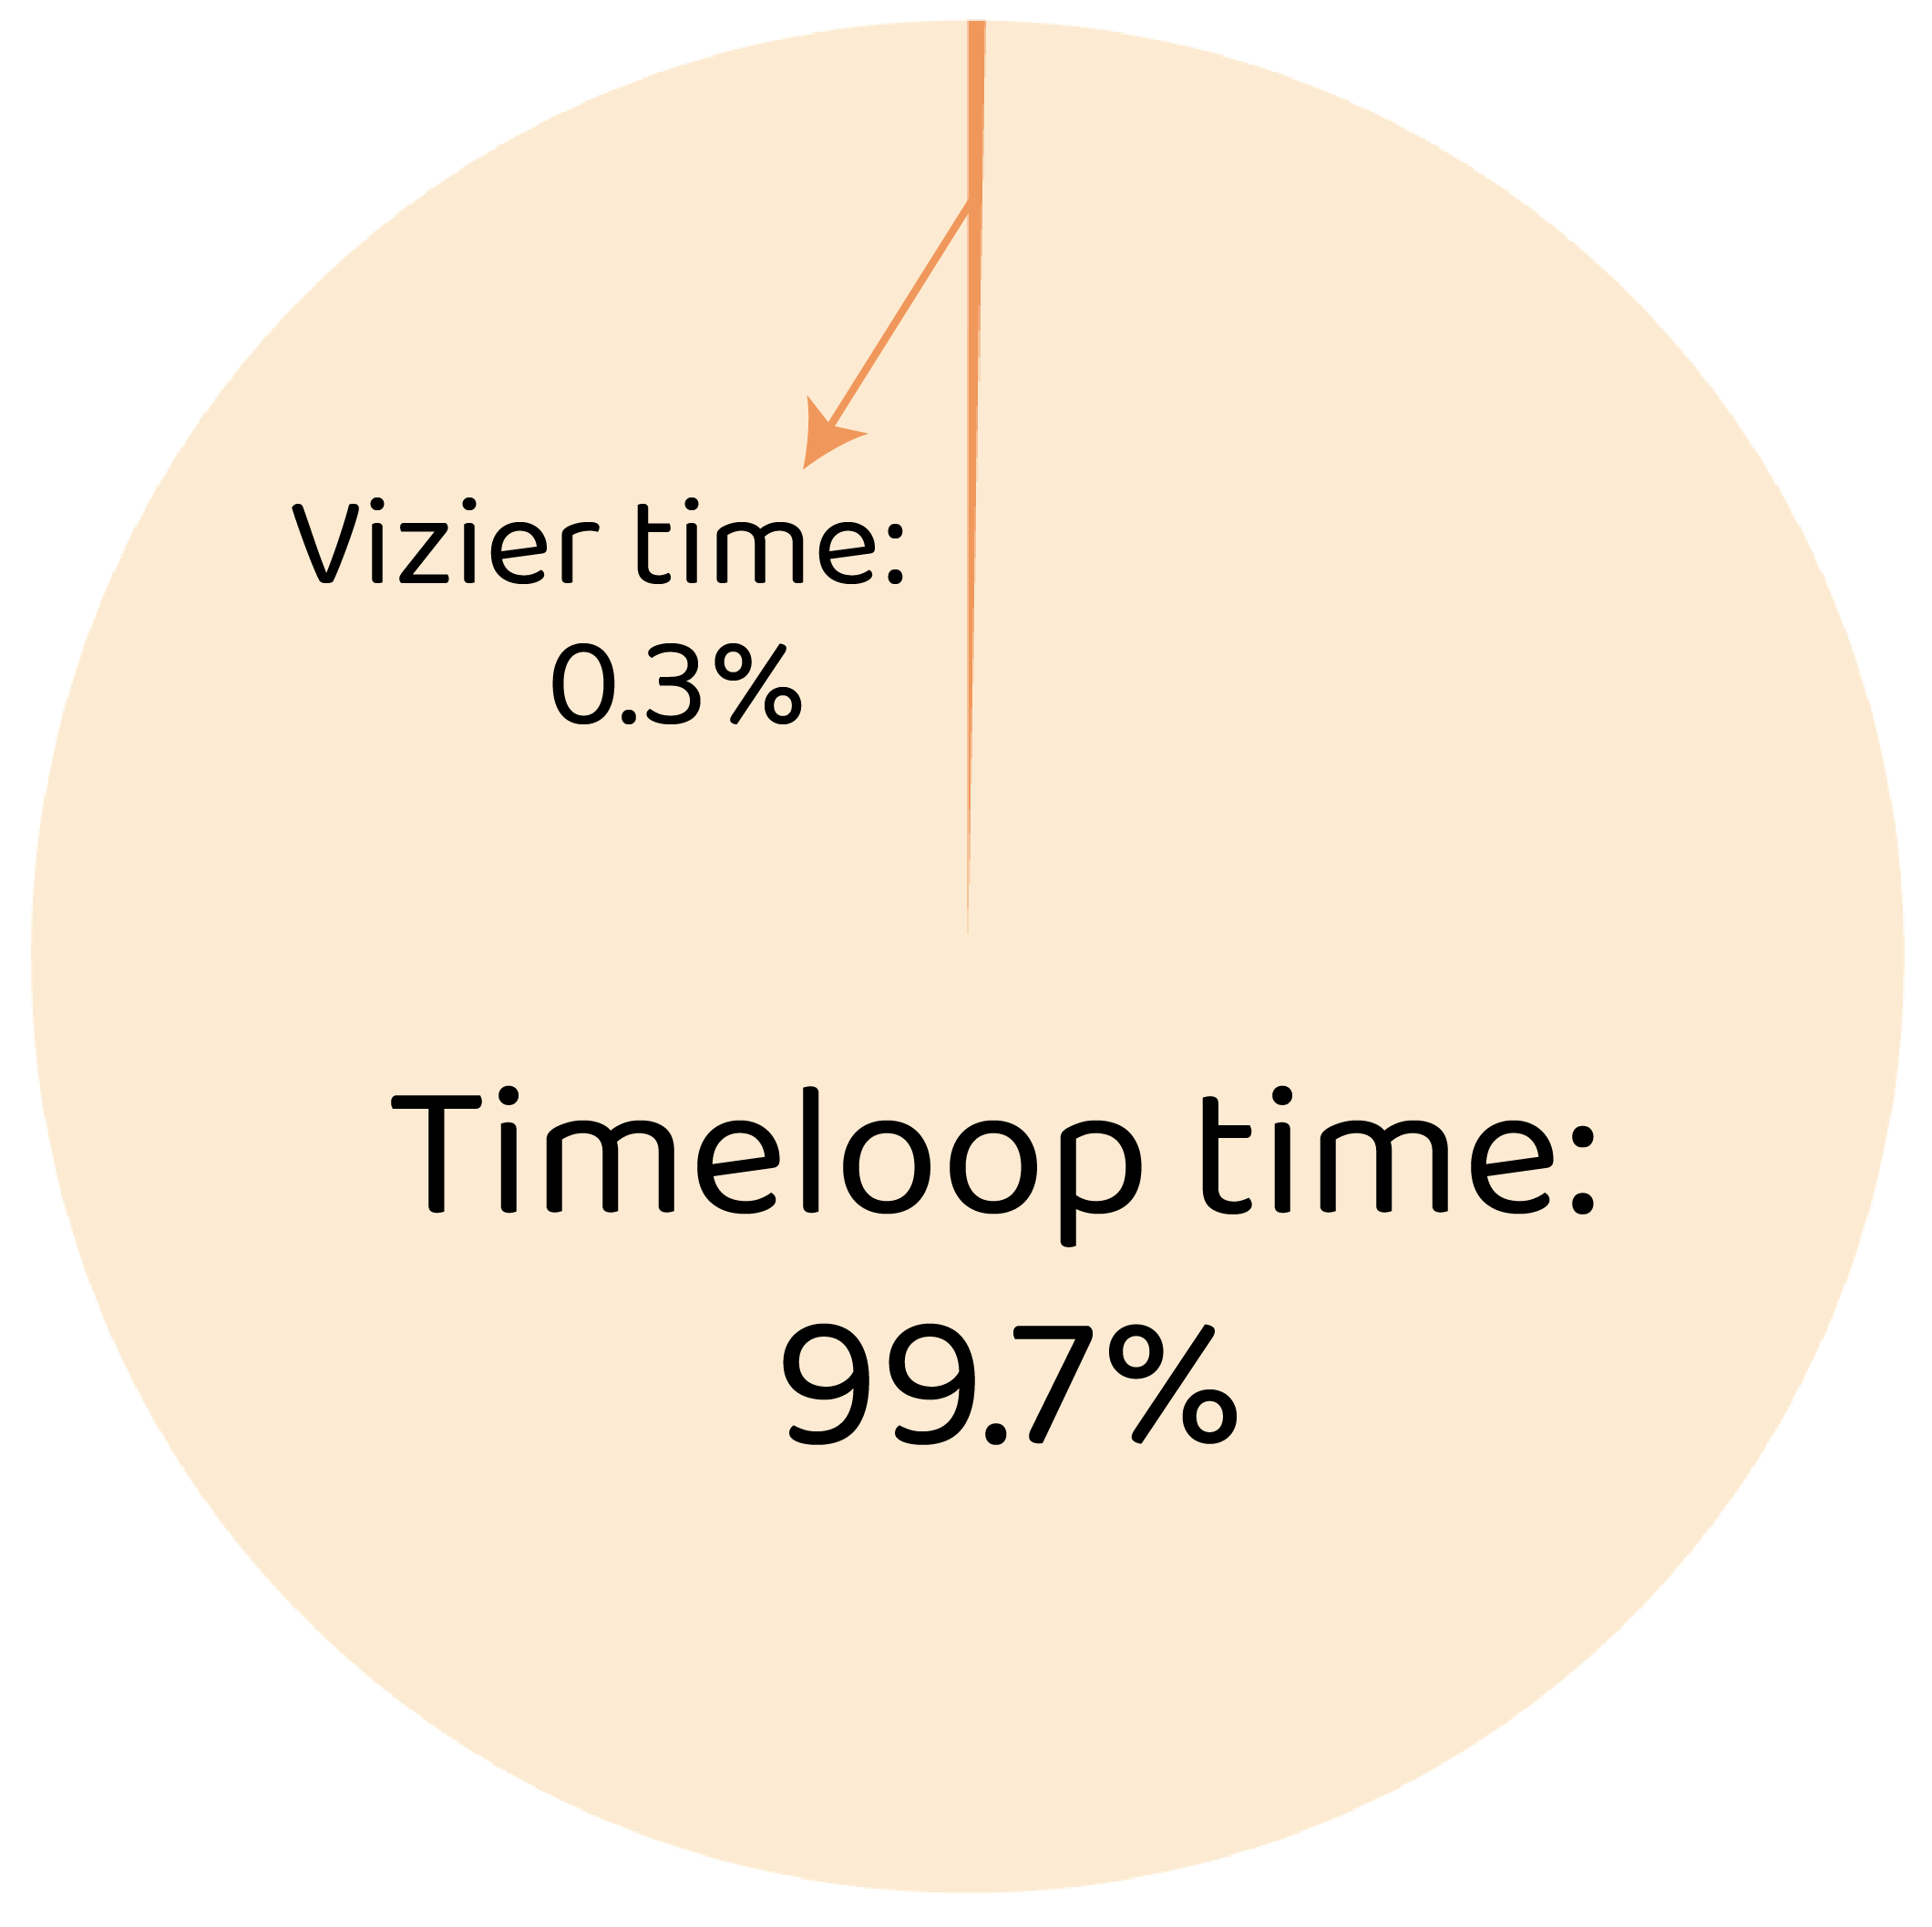
\includegraphics[width=\linewidth]{fig3/timeloop_vs_vizier.png}
%     \caption{Per-trial wall-clock breakdown.}
%     \label{fig:timeloop-time}
%     \vspace{-10pt}
% \end{wrapfigure}
% Despite V0's improvements, it inherits the sequential dependence on external tiling tools (e.g., Timeloop) because it lacks a linear expression for non-linear tiling-fusion interactions. As shown in Figure~\ref{fig:timeloop-time}, Timeloop accounts for over 99\% of per-trial latency, creating a prohibitive bottleneck for multi-thousand-trial searches. To resolve this, CHEETAH-V1 internalizes tiling by precomputing Pareto-pruned configurations and encoding them as decision variables. This removes Timeloop from the critical path, collapsing each trial to a single Vizier-proposal and LP-solve step. We start with introducing the preprocessing stage below before presenting the full formulation in Section~\ref{sec::v1}.

% % The limitations of prior work is still inherited in the V0 formulation due to the difficulty of expressing non-linear relationships as linear constraints. Therefore tiling decisions $(\Tmax_i, \Tmin_i, t_i^k)$ are fixed constants provided by additional software, such as Timeloop. A natural question is whether this sequential dependence also creates a \emph{runtime} bottleneck. Figure~\ref{fig:timeloop-time} confirms that it does: across different models, Timeloop scheduling on average accounts for over 99\% of per-trial wall-clock time, while the Vizier proposal and fusion ILP together consume less than 1\% on average. Because the outer loop requires thousands of trials to converge, the cumulative cost of repeated Timeloop invocations dominates the total search budget. This observation motivates a key design choice in CHEETAH-V1: rather than calling Timeloop online during each trial, we precompute a Pareto-pruned set of tiling configurations once (Section~\ref{sec:pareto}) and encode the tiling selection as decision variables \emph{inside} the LP. This eliminates Timeloop from the per-trial critical path entirely, reducing each trial to a single Vizier-proposal$\,\to\,$LP-solve step.

% % CHEETAH-V1 captures tiling as a \emph{decision variable} inside the LP, enabling the solver to jointly optimize tiling and fusion. We start with describing our preprocessing stage in Section~\ref{sec:pareto} before presenting the full formulation in Section~\ref{sec::v1}.


% \paragraph{Pareto Pruning Pre-Pass} The raw tiling search space for a $7$-dimensional convolution loop with $3$ memory levels is $\mathcal O(10^7)$ configurations per operation. We reduce this to a tractable Pareto-optimal subset $\mathcal{C}_i$ for each operation $i$ via a pre-pass for (1) L1 feasibility where configurations whose tiled working set exceeds L1 scratchpad capacity $C_{L1}$ are discarded; (2) Pareto optimality where a configuration $c$ is retained only if no other configuration achieves both lower $\Tmax_i(c)$ \emph{and} smaller working-set size in the Global Buffer.

% In practice, Pareto pruning reduces $\mathcal O(10^7)$ raw configurations to $|\mathcal{C}_i| \approx 10^2$ to $10^3$ per operation. Timeloop is run once per (operation, configuration) pair, producing the triple $(\Tmin_i(c), \Tmax_i(c), t_i^k(c))$ for each retained configuration $c \in \mathcal{C}_i$. These are precomputed constants---the LP solver makes no Timeloop calls at solve time.

% \paragraph{Time-invariant Pareto fronts.}
% A key observation is that the Pareto front shape is invariant to memory time: configurations are ranked by compute cycles and working-set bytes, neither of which depends on bandwidth. Changing bandwidth rescales the DRAM access cost $t_i^k(c)$ uniformly. This means the Pareto-pruned configuration sets can be precomputed \emph{once} and reused across all Vizier trials that share the same compute configuration class, amortizing the expensive Timeloop precomputation.

% \subsubsection{The Joint CHEETAH-V1 LP Formulation}\label{sec::v1}

% \paragraph{From fixed constants to decision variables.}
% In static and V0 formulations, Timeloop selects a single tiling per operation externally and passes the results to the LP as fixed constants $\Tmax_i$, $\Tmin_i$, $t_i^k$. The DRAM savings from pinning tensor $k$ of operation $i$ is then simply $t_i^k \cdot p_{i,o(i)}^k$---a constant times a variable, which is already linear. V1 brings this tiling choice \emph{inside} the LP by introducing \textbf{tiling selection variables} $y_{i,c} \in [0,1]$, one per Pareto-optimal configuration $c \in \mathcal{C}_i$ from the pre-pass, with the constraint $\sum_c y_{i,c} = 1$ (exactly one configuration is selected per operation). The Timeloop-precomputed constants $\Tmax_i(c)$, $\Tmin_i(c)$, $t_i^k(c)$ now become \emph{per-configuration coefficients} indexed by $c$. This means the DRAM savings term becomes $t_i^k(c) \cdot y_{i,c} \cdot p_{\text{assoc}(i,k),\, o(i)}$. This is a product of \emph{two} decision variables, which is bilinear and cannot be handled by a convex programming directly.
 
% % \paragraph{Linearization via McCormick envelopes.}
% % We linearize this product exactly via the classical McCormick substitution. Specifically,  we introduce \textbf{auxiliary variables} $w_{i,c,k} := y_{i,c} \cdot p_{\text{assoc}(i,k),\, o(i)}$ that represent the joint effect of selecting tiling $c$ \emph{and} pinning tensor $k$, constrained by:
% % \begin{equation}
% % \label{eq:mccormick}
% % \begin{aligned}
% %     w_{i,c,k} &\leq y_{i,c}, \qquad
% %     w_{i,c,k} \leq p_{\text{assoc}(i,k),\, o(i)} \\
% %     w_{i,c,k} &\geq y_{i,c} + p_{\text{assoc}(i,k),\, o(i)} - 1, \qquad
% %     w_{i,c,k} \geq 0
% % \end{aligned}
% % \end{equation}
% % Since both factors lie in $[0,1]$, these four constraints force $w_{i,c,k} = y_{i,c} \cdot p$ at any integer vertex, requiring no manually tuned constants. Together, $y_{i,c}$ and $w_{i,c,k}$ account for 1.6M of the 2.08M variables in the \Vone~ LP (Table~\ref{tab:v1_scale}). \todo{change to MoE?}

% \paragraph{Linearization via McCormick envelopes.}
% We linearize this product exactly via the classical McCormick substitution \citep{mccormick1976computability}. Specifically, we introduce \textbf{auxiliary variables} $w_{i,c,k} := y_{i,c} \cdot p_{\text{assoc}(i,k),\, o(i)}$ that represent the joint effect of selecting tiling $c$ \emph{and} pinning tensor $k$, constrained by:
% \begin{equation}
% \label{eq:mccormick}
% \begin{aligned}
%     w_{i,c,k} &\leq y_{i,c}, \qquad
%     w_{i,c,k} \leq p_{\text{assoc}(i,k),\, o(i)} \\
%     w_{i,c,k} &\geq y_{i,c} + p_{\text{assoc}(i,k),\, o(i)} - 1, \qquad
%     w_{i,c,k} \geq 0
% \end{aligned}
% \end{equation}
% Since both factors lie in $[0,1]$, these four constraints force $w_{i,c,k} = y_{i,c} \cdot p$ at any integer vertex, requiring no manually tuned constants. Together, $y_{i,c}$ and $w_{i,c,k}$ constitute the majority of V1's decision variables (Table~\ref{tab:v1_scale}).
 

% % \paragraph{Full formulation.}
% % Combining tiling selection, time-indexed placement, rematerialization, and McCormick linearization, the full V1  formulation is:

% % \begin{equation}
% % % \label{eq:v1}
% % \begin{aligned}
% % \min \quad & \sum_{i \in \mathcal{N}} T_i + \sum_{i \in \mathcal{N}} \sum_{t \in \mathcal{T}} c_i^{\text{remat}} \, r_{i,t} \\[4pt]
% % \text{s.t.} \quad
% % & \sum_{c \in \mathcal{C}_i} y_{i,c} = 1 & \forall\, i \in \mathcal{N} \\[3pt]
% % & T_i \geq \sum_{c \in \mathcal{C}_i} \Tmax_i(c)\, y_{i,c} - \sum_{c \in \mathcal{C}_i} \sum_{k} t_i^k(c)\, w_{i,c,k} & \forall\, i \in \mathcal{N} \\[3pt]
% % & T_i \geq \sum_{c \in \mathcal{C}_i} \Tmin_i(c)\, y_{i,c} & \forall\, i \in \mathcal{N} \\[3pt]
% % & w_{i,c,k} \leq y_{i,c} & \forall\, i, c, k \\
% % & w_{i,c,k} \leq p_{\text{assoc}(i,k),\, o(i)} & \forall\, i, c, k \\
% % & w_{i,c,k} \geq y_{i,c} + p_{\text{assoc}(i,k),\, o(i)} - 1 & \forall\, i, c, k \\[3pt]
% % & \sum_{e \in \mathcal{E}} d_e\, p_{e,t} + \sum_{i \in \mathcal{N}} d_i^W\, p_{i,t}^W \leq \CGM & \forall\, t \in \mathcal{T} \\[3pt]
% % & p_{e,t} \leq p_{e,t-1} + r_{\text{src}(e),\, t} & \forall\, e, t > o(\text{src}(e)) \\
% % & p_{i,t}^W \leq p_{i,t-1}^W & \forall\, i, t > o(i) \\[3pt]
% % & r_{i,t} = 0 & \forall\, i, t \leq o(i) \\
% % & r_{i,t} \leq p_{e,t} & \forall\, e \in \text{in}(i), t > o(i) \\
% % & r_{i,t} \leq p_{i,t}^W & \forall\, i, t > o(i) \\[3pt]
% % & T_i, p_{e,t}, p_{i,t}^W, r_{i,t}, w_{i,c,k} \geq 0 &
% % \end{aligned}
% % \tag{\textcolor{skyblue}{V1}}\label{eq:v1}
% % \end{equation}
% % full formulation below in appendix 
% % \begin{equation}
% % \begin{aligned}
% % \min \quad & \sum_{i \in \mathcal{N}} T_i + \sum_{i \in \mathcal{N}} \sum_{t \in \mathcal{T}} c_i^{\text{remat}} \, r_{i,t} \\[4pt]
% % \text{s.t.} \quad
% % & \sum_{c \in \mathcal{C}_i} y_{i,c} = 1 & \forall\, i \in \mathcal{N} \\[3pt]
% % & T_i \geq \max\!\left(\sum_{c \in \mathcal{C}_i} \Tmin_i(c)\, y_{i,c},\;\; \sum_{c \in \mathcal{C}_i} \Tmax_i(c)\, y_{i,c} - \sum_{c \in \mathcal{C}_i} \sum_{k} t_i^k(c)\, w_{i,c,k}\right) & \forall\, i \in \mathcal{N} \\[3pt]
% % & w_{i,c,k} \leq y_{i,c}, \quad w_{i,c,k} \leq p_{\text{assoc}(i,k),\, o(i)}, \quad w_{i,c,k} \geq y_{i,c} + p_{\text{assoc}(i,k),\, o(i)} - 1 & \forall\, i, c, k \\[3pt]
% % & \sum_{e \in \mathcal{E}} d_e\, p_{e,t} + \sum_{i \in \mathcal{N}} d_i^W\, p_{i,t}^W \leq \CGM & \forall\, t \in \mathcal{T} \\[3pt]
% % & p_{e,t} \leq p_{e,t-1} + r_{\text{src}(e),\, t} & \forall\, e,\, t > o(\text{src}(e)) \\
% % & p_{i,t}^W \leq p_{i,t-1}^W & \forall\, i,\, t > o(i) \\[3pt]
% % & r_{i,t} = 0 \;\; \forall\, t \leq o(i); \quad r_{i,t} \leq \min\!\big(p_{e,t},\, p_{i,t}^W\big) \;\; \forall\, e \in \text{in}(i),\, t > o(i) \\[3pt]
% % & T_i,\, p_{e,t},\, p_{i,t}^W,\, r_{i,t},\, w_{i,c,k} \geq 0 &
% % \end{aligned}
% % \tag{\textcolor{skyblue}{V1}}\label{eq:v1}
% % \end{equation}

% \paragraph{Variable and constraint digest.}
% The V1 formulation inherits all the features of the V0 formulation, and additionally captures tiling by introducing selection variables
% $y_{i,c} \in [0,1]$, constrained by $\sum_c y_{i,c} = 1$, to choose
% from $|\mathcal{C}_i|$ Pareto-optimal configurations.
% Each configuration defines compute costs $T_i^{\max}(c)$,
% $T_i^{\min}(c)$, and per-tensor DRAM savings $t_i^k(c)$.
% We linearize the resulting bilinear DRAM-savings term exactly via
% McCormick auxiliary variables $w_{i,c,k}$, which enforce $w_{i,c,k} \;=\; y_{i,c} \cdot p_{\mathrm{assoc}(i,k),\,o(i)}$ at integer vertices without a relaxation gap.

% Per-operation latency $T_i$ is lower-bounded by the weighted
% configuration floor $\sum_c T_i^{\min}(c)\, y_{i,c}$ and the weighted
% off-chip cost $\sum_c T_i^{\max}(c)\, y_{i,c}$ minus achievable savings
% $\sum_{c,k} t_i^k(c)\, w_{i,c,k}$.
% This coupling enables the solver to accept sub-optimal local tiling
% (higher $T_i^{\max}$) if its smaller memory footprint unlocks global
% fusion gains that outweigh the compute-utilization loss.
% Capacity and persistence constraints carry over from V0, utilizing
% edge-indexed placement $p_{e,t}$ to handle multi-fanout nodes.
% For DeepSeek-V3, the V1 LP scales to approximately $2{,}504{,}019$ variables, $2{,}983{,}450$ constraints, and $6{,}094{,}156$ non-zeros. Table~\ref{tab:v1_scale} provides a representative breakdown, Table~\ref{tab:comparison} summarizes features of each more powerful formulation; full per-model sizes are in Table~\ref{tab:exp1_lp_sizes} and \ref{tab:exp2_cluster_lp_sizes}. 



% % The V1 formulation extends V0 by making the tiling configuration a decision variable. The selection variables $y_{i,c} \in [0,1]$, with $\sum_c y_{i,c} = 1$, choose among $|\mathcal{C}_i|$ Pareto-optimal tiling configurations precomputed by Timeloop (Section~\ref{sec:pareto}). Each configuration $c$ determines the operation's compute cost $T_i^{\max}(c)$, on-chip floor $T_i^{\min}(c)$, and per-tensor DRAM savings $t_i^k(c)$.
% % The DRAM savings term $t_i^k(c) \cdot y_{i,c} \cdot p_{\text{assoc}(i,k),\,o(i)}$ 
% % is bilinear in the tiling selection and placement variables; we linearize it 
% % via McCormick auxiliary variables $w_{i,c,k}$, constrained by 
% % $w_{i,c,k} \leq y_{i,c}$, $w_{i,c,k} \leq p_{\text{assoc}(i,k),\,o(i)}$, and 
% % $w_{i,c,k} \geq y_{i,c} + p_{\text{assoc}(i,k),\,o(i)} - 1$. 
% % These three inequalities force $w_{i,c,k} = y_{i,c} \cdot p_{\text{assoc}(i,k),\,o(i)}$ 
% % at any integer-feasible point (\cref{prop:mccormick_exact}), so the LP exactly captures the 
% % bilinear interaction without introducing any relaxation gap at integer vertices.
% % The $T_i$ lower bound now takes the maximum of two configuration-dependent terms: the weighted on-chip floor $\sum_c T_i^{\min}(c)\, y_{i,c}$ and the weighted off-chip cost minus achievable savings $\sum_c T_i^{\max}(c)\, y_{i,c} - \sum_{c,k} t_i^k(c)\, w_{i,c,k}$.
% % This coupling is the core novelty of V1: the solver can accept a tiling with higher $T_i^{\max}(c)$ (lower compute utilization) if its smaller working set enables pinning decisions that reduce total DRAM traffic by more than the utilization loss.
% % All remaining constraints---memory capacity, persistence, and rematerialization---carry over from V0 with edge-indexed placement variables $p_{e,t}$ replacing per-tensor $p_{i,t}^k$ to correctly handle skip connections and multi-fanout nodes. For our largest workload, DeepSeek-V3 ($L \approx 6{,}300$ operations), the V1 LP contains approximately 2.5M variables, 3.0M constraints, and 6.1M nonzeros. Table~\ref{tab:v1_scale} provides a representative breakdown; full per-model sizes are in Table~\ref{tab:v1_scale}. 
% % \paragraph{Key constraint interactions.}
% % The execution-time constraints (lines 2--3: the upper and lower bounds for $T_i$) capture the central trade-off that is unique to \Vone: the LP must commit to a tiling configuration $c$ (via $y_{i,c}$) that sets both the baseline compute cost $\Tmax_i(c)$ and the achievable DRAM savings $t_i^k(c)$. A configuration with smaller tiles may have higher $\Tmax_i(c)$ (lower compute utilization) but smaller working sets, enabling more aggressive pinning. The LP balances these trade-offs simultaneously---precisely the cross-stage interaction that the sequential pipeline cannot discover.
 
% % The edge-indexed persistence constraint (line 8: $p_{e,t} \leq p_{e,t-1} + r_{\text{src}(e),\, t}$) and the memory capacity constraint (line 7: lower bound on $\CGM$) are inherited from \Vzero, which introduced per-edge placement variables $p_{e,t}$ to correctly model skip connections. \Vone~ extends this by coupling edge sizes to the tiling selection---since different configurations $c$ produce different activation working sets, the LP can now jointly reason about how tiling choices affect memory pressure across skip connections.


% \begin{figure}[ht!]
% \begin{minipage}[t]{0.48\textwidth}
% \vspace{0pt}
% \centering
% \captionof{table}{V1 variable and constraint counts
% (representative, DeepSeek-V3).}
% \label{tab:v1_scale}
% \footnotesize
% \begin{tabular}{@{}ll@{}}
% \toprule
% \textbf{Variable} & \textbf{Role} \\
% \midrule
% $T_i$       & Per-operation execution time \\
% $y_{i,c}$   & Tiling config selection ($|\mathcal{C}_i|$ options) \\
% $p_{e,t}$   & Edge-indexed activation placement \\
% $p_{i,t}^W$ & Weight placement \\
% $r_{i,t}$   & Rematerialization indicator \\
% $w_{i,c,k}$ & McCormick auxiliaries ($y_{i,c} \cdot p$) \\
% % \midrule
% % \multicolumn{2}{@{}l}{\textbf{DeepSeek-V3 totals}
% %                        ($L \approx 6{,}300$)} \\
% % \midrule
% % Variables   & $2{,}504{,}019$ \\
% % Constraints & $2{,}983{,}450$ \\
% % Nonzeros    & $6{,}094{,}156$ \\
% \bottomrule
% \end{tabular}
% \end{minipage}%
% \hspace{0.02\textwidth}%
% \begin{minipage}[t]{0.48\textwidth}
% \vspace{0pt}
% \centering
% \captionof{table}{Comparison of static, V0, and V1 formulations.}
% \label{tab:comparison}
% \footnotesize
% \begin{tabular}{@{}lccc@{}}
% \toprule
% \textbf{Property} & \textbf{Static} & \textbf{V0} & \textbf{V1} \\
% \midrule
% Joint tiling + fusion    & $\times$ & $\times$   & \checkmark \\
% Time-indexed placement   & $\times$ & \checkmark & \checkmark \\
% Rematerialization        & $\times$ & \checkmark & \checkmark \\
% Relaxed skip connections & $\times$ & Partial    & \checkmark \\
% \bottomrule
% \end{tabular}

% \medskip
% \raggedright
% \footnotesize
% % \textbf{Comparison across formulations.}
% % Table~\ref{tab:comparison} summarizes the progression from the
% % static formulation through V0 to V1.
% \end{minipage}
% \end{figure}


% % \begin{table}[ht!]
% % \centering
% % \caption{V1 variable and constraint counts (representative, DeepSeek-V3).}
% % \label{tab:v1_scale}
% % \small
% % \begin{tabular}{lrl}
% % \toprule
% % \textbf{Variable} & \textbf{Role} \\
% % \midrule
% % $T_i$ & Per-operation execution time \\
% % $y_{i,c}$ & Tiling configuration selection ($|\mathcal{C}_i|$ options per op) \\
% % $p_{e,t}$ & Edge-indexed activation placement \\
% % $p_{i,t}^W$ & Weight placement \\
% % $r_{i,t}$ & Rematerialization indicator \\
% % $w_{i,c,k}$ & McCormick auxiliaries ($y_{i,c} \cdot p$) \\
% % \midrule
% % \multicolumn{2}{l}{\textbf{DeepSeek-V3 totals} ($L \approx 6{,}300$)} \\
% % \midrule
% % Variables & 2,504,019 \\
% % Constraints & 2,983,450 \\
% % Nonzeros & 6,094,156 \\
% % \bottomrule
% % \end{tabular}
% % \end{table}
% % \paragraph{Comparison across formulations.}
% % Table~\ref{tab:comparison} summarizes the progression from static through V0 to V1.
% % \begin{table}[ht!]
% % \centering
% % \caption{Comparison of static, V0, and V1 formulations.}
% % \label{tab:comparison}
% % \small
% % \begin{tabular}{lccc}
% % \toprule
% % \textbf{Property} & \textbf{static} & \textbf{V0} & \textbf{V1} \\
% % \midrule
% % Joint tiling + fusion & \texttimes & \texttimes & \checkmark \\
% % Time-indexed placement & \texttimes & \checkmark & \checkmark \\
% % Rematerialization & \texttimes & \checkmark & \checkmark \\
% % Relaxed skip connections & \texttimes & Partial & \checkmark \\
% % % Config-dependent DRAM savings & \texttimes & \texttimes & \checkmark \\ 
% % % Bilinear linearization & --- & --- & McCormick \\
% % \bottomrule
% % \end{tabular}
% % \end{table}

% % \paragraph{Structural invariance for efficient LLM integration.}
% % A practical advantage of both our LP formulations is that the constraint matrix sparsity pattern is invariant across hardware configurations---only the numerical coefficients change. This means:
% % \begin{itemize}
% %     \item The LP solver's preconditioner can be designed once per neural network model and reused across all Vizier trials.
% %     \item An LLM-Architect can reason about constraint structure (which constraints are binding, which variables are fractional) without needing to understand the full LP.
% %     \item Warm-starting from a previous trial's LP solution is straightforward since the variable indexing is stable.
% % \end{itemize}

% \subsection{Strategic Intelligence: LLM-Guided Outer Search}
% \label{sec:llm_outer}
% We use Google Vizier as a black-box Bayesian optimizer to propose hardware configurations. While effective, vanilla Vizier treats search as pure function optimization, often requiring thousands of iterations to identify suboptimal regions without leveraging structural hardware-workload knowledge. To address this, we introduce an LLM-guided outer-loop controller based on SkyDiscovery that reasons about co-design decisions. By learning from a causal ledger of past trials and Lagrangian dual signals from the LP solver, the LLM proposes meaningful, constrained search-space candidates. This integration is enabled by the CHEETAH-V1 formulation, which removes the Timeloop bottleneck to reduce trial times from days to hours.The LLM-Architect reduces wasted trials by intelligently steering Vizier’s search without altering the inner solver or its optimality certificates. In this hybrid loop, the LLM determines global architectural regions, Vizier performs local Bayesian optimization within those patches, and the large-scale V1 LP solver evaluates each concrete candidate. The LLM-Architect loop proceeds as follows: 
% % We use Vizier as a black-box Bayesian optimizer to propose candidate hardware configurations. While effective, Vizier search strategies (LCS, UCB, etc) requires thousands of iterations explore and learn which regions are suboptimal and treats the search as a pure function optimization problem without leveraging structural knowledge about hardware-workload interactions.
% % We leverage an LLM-guided outer-loop controller that learns from logs of thousands of past co-design trials to propose meaningful search-space candidates for Vizier. This is a SkyDiscovery based outer LLM layer which reasons about hardware-software co-design decisions and learns from a causal ledger of constantly updated logs across trials, as well as feed-back signal such as dual variables through the LP solve. This is possible for CHEETAH-V1 LP formulation, since it removes the Timeloop-in-the-loop constraint, thus reducing the co-design problem from days to hours, and permitting the LLM outer loop. 

% % The LLM-Architect does not change the inner solver, and retains all the optimal certificates of the V1 LP formulation, but intelligently changes where the Vizier outer hardware optimizer searches to reduce wasted trials. The LLM proposes global decisions to determine constrained regions of the hardware search space; Vizier then performs local Bayesian optimization inside those regions; which then passes downstream into a large scale LP solver for the V1 formulation to evaluate each concrete candidate. The LLM-Architect loop proceeds as follows:

% \begin{enumerate}[leftmargin=1.6em, itemsep=4pt]

% \item \textbf{Extraction.}
% Deterministic scripts summarize recent trials into a \emph{Causal
% Ledger}. Each record includes hardware parameters, validity, Perf/TDP,
% LP cycles, capacity duals/slacks, bandwidth sensitivity, MFU, memory
% utilization, roofline gap, failure class, and LP solver metrics.

% \item \textbf{Context building.}
% The last $N$ trials and the Causal Ledger are compressed into a compact
% JSON context for the Architect. The context emphasizes empirical
% feasibility, observed invalid regions, best known valid designs, and
% physical audit signals.

% \item \textbf{Architect.}
% The online Architect, implemented as Qwen2.5-7B-Instruct with a LoRA
% adapter trained on past trial logs, diagnoses the dominant bottleneck
% and emits a campaign patch. The patch constrains macro-architectural
% search decisions such as Global Memory, DRAM bandwidth, total MACs,
% systolic shape, PE grid, and batch size. A larger teacher model,
% DeepSeek-V3.2, was used offline to generate or critique campaign labels
% but is not in the live loop.

% \item \textbf{Campaign validation.}
% A deterministic validator clips or rejects the LLM patch to enforce
% legal hardware ranges, TDP and area limits, MAC caps, CGM feasibility
% floors, compute/bandwidth coupling, and roofline constraints. This
% prevents the LLM from proposing physically implausible regions such as
% maximum-MAC/minimum-bandwidth designs.

% \item \textbf{Local optimization.}
% Vizier is initialized inside the validated patch and warm-started with
% prior trials that lie in the same region. Vizier then samples concrete
% hardware candidates within the approved campaign. The LLM therefore
% chooses the high-level architectural neighbourhood, while Vizier
% performs local adaptive optimization.

% \item \textbf{Unified V1 evaluation.}
% The large-scale LP solver evaluates each candidate by solving the V1
% joint tiling-fusion-placement LP using saved Pareto $\mathcal{C}$-sets.
% It returns the objective, cycles, selected tiling configurations,
% placement/rematerialization decisions, dual/slack summaries, and
% solver-quality diagnostics.

% \item \textbf{Roofline audit.}
% A deterministic Roofline Auditor checks whether the predicted latency
% is physically plausible. For each candidate we compute
% \begin{align}
%     t_{\text{compute}} &=
%         \frac{\text{useful FLOPs}}{\text{peak FLOPs/s}},
%     \qquad
%     t_{\text{memory}}  =
%         \frac{\text{post-placement DRAM bytes}}{\text{peak bandwidth}},
%     \nonumber\\
%     t_{\text{ideal}}   &=
%         \max\!\left(t_{\text{compute}},\, t_{\text{memory}}\right).
%     \label{eq:roofline_audit}
% \end{align}
% A candidate is rejected if the solver-reported latency falls below this
% lower bound, or if MFU or memory utilization exceeds 1.0 within
% tolerance.

% \item \textbf{Ledger update.}
% The loop records the campaign hypothesis, intervention, observed
% invalid-rate change, MFU change, roofline validity, and best Perf/TDP
% change. The ledger also records forbidden regions when a campaign
% produces excessive invalid trials.

% \end{enumerate}

% \noindent The Architect receives workload summaries, invalid-rate
% history, MFU, roofline signals, prior valid regions, normalized LP duals,
% and bandwidth sensitivities. The system starts from a safe empirically
% valid patch and permits duals only to make bounded edits, such as raising
% the CGM floor, increasing bandwidth, reducing MAC count, or changing
% systolic shapes. The validator rejects any dual-guided patch that
% excludes known high-performing valid regions or predicts a substantially
% worse feasible rate. This provides controlled architectural feedback in
% addition to prompt input.


% % \todo{Expand this section once the LLM+RL experimental protocol is finalized. Key questions to address: (1) Which LLM is used and how is it prompted? (2) How are LLM proposals integrated with Vizier's Bayesian model? (3) What is the sample efficiency improvement over pure Vizier?}





% edit for page limit 
\section{Methodology}
\label{sec:methods}
We present the \textbf{CHEETAH} (\acroletter{C}o-designed \acroletter{H}ardware \acroletter{E}xploration via \acroletter{E}fficient \acroletter{T}hroughput and \acroletter{H}ybrid-search) framework in three parts: Section~\ref{sec:v0} introduces CHEETAH-V0, which extends the static fusion ILP with time-indexed placement and rematerialization. Section~\ref{sec:v1} presents CHEETAH-V1, which jointly optimizes tiling and fusion via McCormick linearization. Section~\ref{sec:llm_outer} describes the LLM-Architect outer loop. Appendix~\ref{sec:theory} provides theoretical analysis on the exactness of our mathematical modeling, and Appendix~\ref{app:invar} provides details on structured constraint matrices, and Appendix~\ref{app:llm_loop} presents the LLM Architect outer loop design details.

\paragraph{What the program optimizes over: static structure, dynamic dimensions.}
A single model's compute graph is \emph{structurally static}: the layers and
dependencies of, say, Llama-70B do not change from request to request. What
varies at inference is the \emph{data and the dimensions}: sequence length, batch
size, mixture-of-experts routing, and the number of decode steps. CHEETAH is
therefore a \emph{design-time} program, solved offline over the static structure
at a representative operating point (context, batch, generation length) together
with workload statistics (per-expert routing frequency $f_e$, the prefix
cache-hit profile). The chip is designed once for the operating envelope, not
re-solved per request. Data-dependent routing enters as a distribution: the
expected number of distinct experts touched at the deployed batch (a
balls-in-bins occupancy model), with load-balancing and token-drop caps bounding
the tail. When a deployment spans a wide range of shapes, the same program is
solved over a distribution of operating points (a few weighted
$(\text{context},\text{batch},\text{routing})$ samples) to yield a design robust
across the dynamic range rather than overfit to one point; such a stochastic
objective is the weighted sum $\sum_k w_k T^{(k)}$ over the samples, and the
robust one the epigraph $T \ge T^{(k)}$ for every sample; both are linear rows
of the same LP. Per-request scheduling of one realized dynamic graph is
a separate problem (a fixed-hardware compiler), not the co-design program studied
here.


% \subsection{\Vzero~: Multi-Period Placement with Rematerialization}
\subsection{CHEETAH-V0: Multi-Period Placement with Rematerialization}
\label{sec:v0}

Our first extension models the neural network's (NN) execution as a sequence of $T$ discrete timesteps (one per operation in execution order). This decides at which time, which tensor is pinned, evicted, or recomputed to optimally minimize cycle counts. The key features are:

\paragraph{Time-indexed placement.}
Instead of a single binary $p_i^k$ per tensor, we introduce $p_{i,t}^k \in [0,1]$ for each tensor $k$ of layer $i$ at each timestep $t$. A tensor can be pinned at timestep $t=5$, and evicted at $t=10$. This models a dynamic memory manager within a single inference pass.

\paragraph{Rematerialization.}
Rather than always paying DRAM bandwidth to reload an evicted tensor, we introduce variables $r_{i,t} \in [0,1]$ indicating that layer $i$ is recomputed at timestep $t$ to restore its output to the Global Buffer. This is particularly valuable for models such as EfficientNet, where depthwise convolutions account for only ${\sim}5\%$ of total FLOPs but produce large activation tensors. Recomputing a depthwise layer to avoid re-reading 6\,MiB from DRAM at 256\,GB/s can be faster than the DRAM reload itself.

\paragraph{Relaxed skip-connection handling.}
CHEETAH-V0 lifts the baseline's restriction to consecutive operations by using edge-indexed placement variables $p_{e,t}$ for each edge $e \in \mathcal{E}$, correctly modeling multi-fanout skip connections where consumers independently benefit from on-chip data.

The CHEETAH-V0 LP formulation is:
\begin{equation}
% \label{eq:v0}
\begin{aligned}
\min \quad & \sum_{i \in \mathcal{N}} T_i + \sum_{i \in \mathcal{N}} \sum_{t \in \mathcal{T}} c_i^{\text{remat}} \, r_{i,t} \\
\text{s.t.} \quad
& T_i \geq \Tmax_i - \sum_{k \in \{I,O,W\}} t_i^k \cdot p_{i,o(i)}^k & \forall\, i \in \mathcal{N} \\
& T_i \geq \Tmin_i & \forall\, i \in \mathcal{N} \\
& \sum_{i \in \mathcal{N}} \sum_{k} d_i^k \, p_{i,t}^k \leq \CGM & \forall\, t \in \mathcal{T} \\
& p_{i,t}^k \leq p_{i,t-1}^k + r_{i,t} & \forall\, i, t, k \in \{I,O\} \\
& p_{i,t}^W \leq p_{i,t-1}^W & \forall\, i, t \\
& r_{i,t} = 0 & \forall\, i, t \leq o(i) \\
& 0 \leq p_{i,t}^k, r_{i,t} \leq 1 &
\end{aligned}
\tag{V0}\label{eq:v0}
\end{equation}


where $o(i)$ is the execution order of operation $i$, $d_i^k$ is the byte size of tensor $k$ for layer $i$, and $c_i^{\text{remat}}$ is the recomputation cost.

\paragraph{Variable and constraint digest.}
The objective minimizes total execution time $\sum_i T_i$ plus rematerialization costs. Per-operation latency $T_i$ is lower-bounded by the on-chip floor $T_i^{\min}$ and the off-chip time $T_i^{\max}$ adjusted for DRAM savings from pinned tensors. Persistence constraints enforce monotone eviction for weights and allow recomputation-based restoration for activations; rematerialization is only permitted post-execution and requires on-chip availability of both inputs and weights.
For DeepSeek-V3 ($L \approx 6{,}300$), this formulation yields a large-scale program with approximately 3.3M variables and 3.7M constraints. See Appendix~\ref{sec:lps} for a detailed breakdown. 


% \subsection{\textcolor{skyblue}{V1}: Joint Tiling and Fusion via McCormick Linearization}
% \vspace{-6pt}
\subsection{CHEETAH-V1: Joint Tiling, Fusion, and Hardware Sizing Inside the Program}
\label{sec:v1}

\begin{wrapfigure}{r}{0.2\linewidth}
    % \vspace{-12pt}
    \centering
    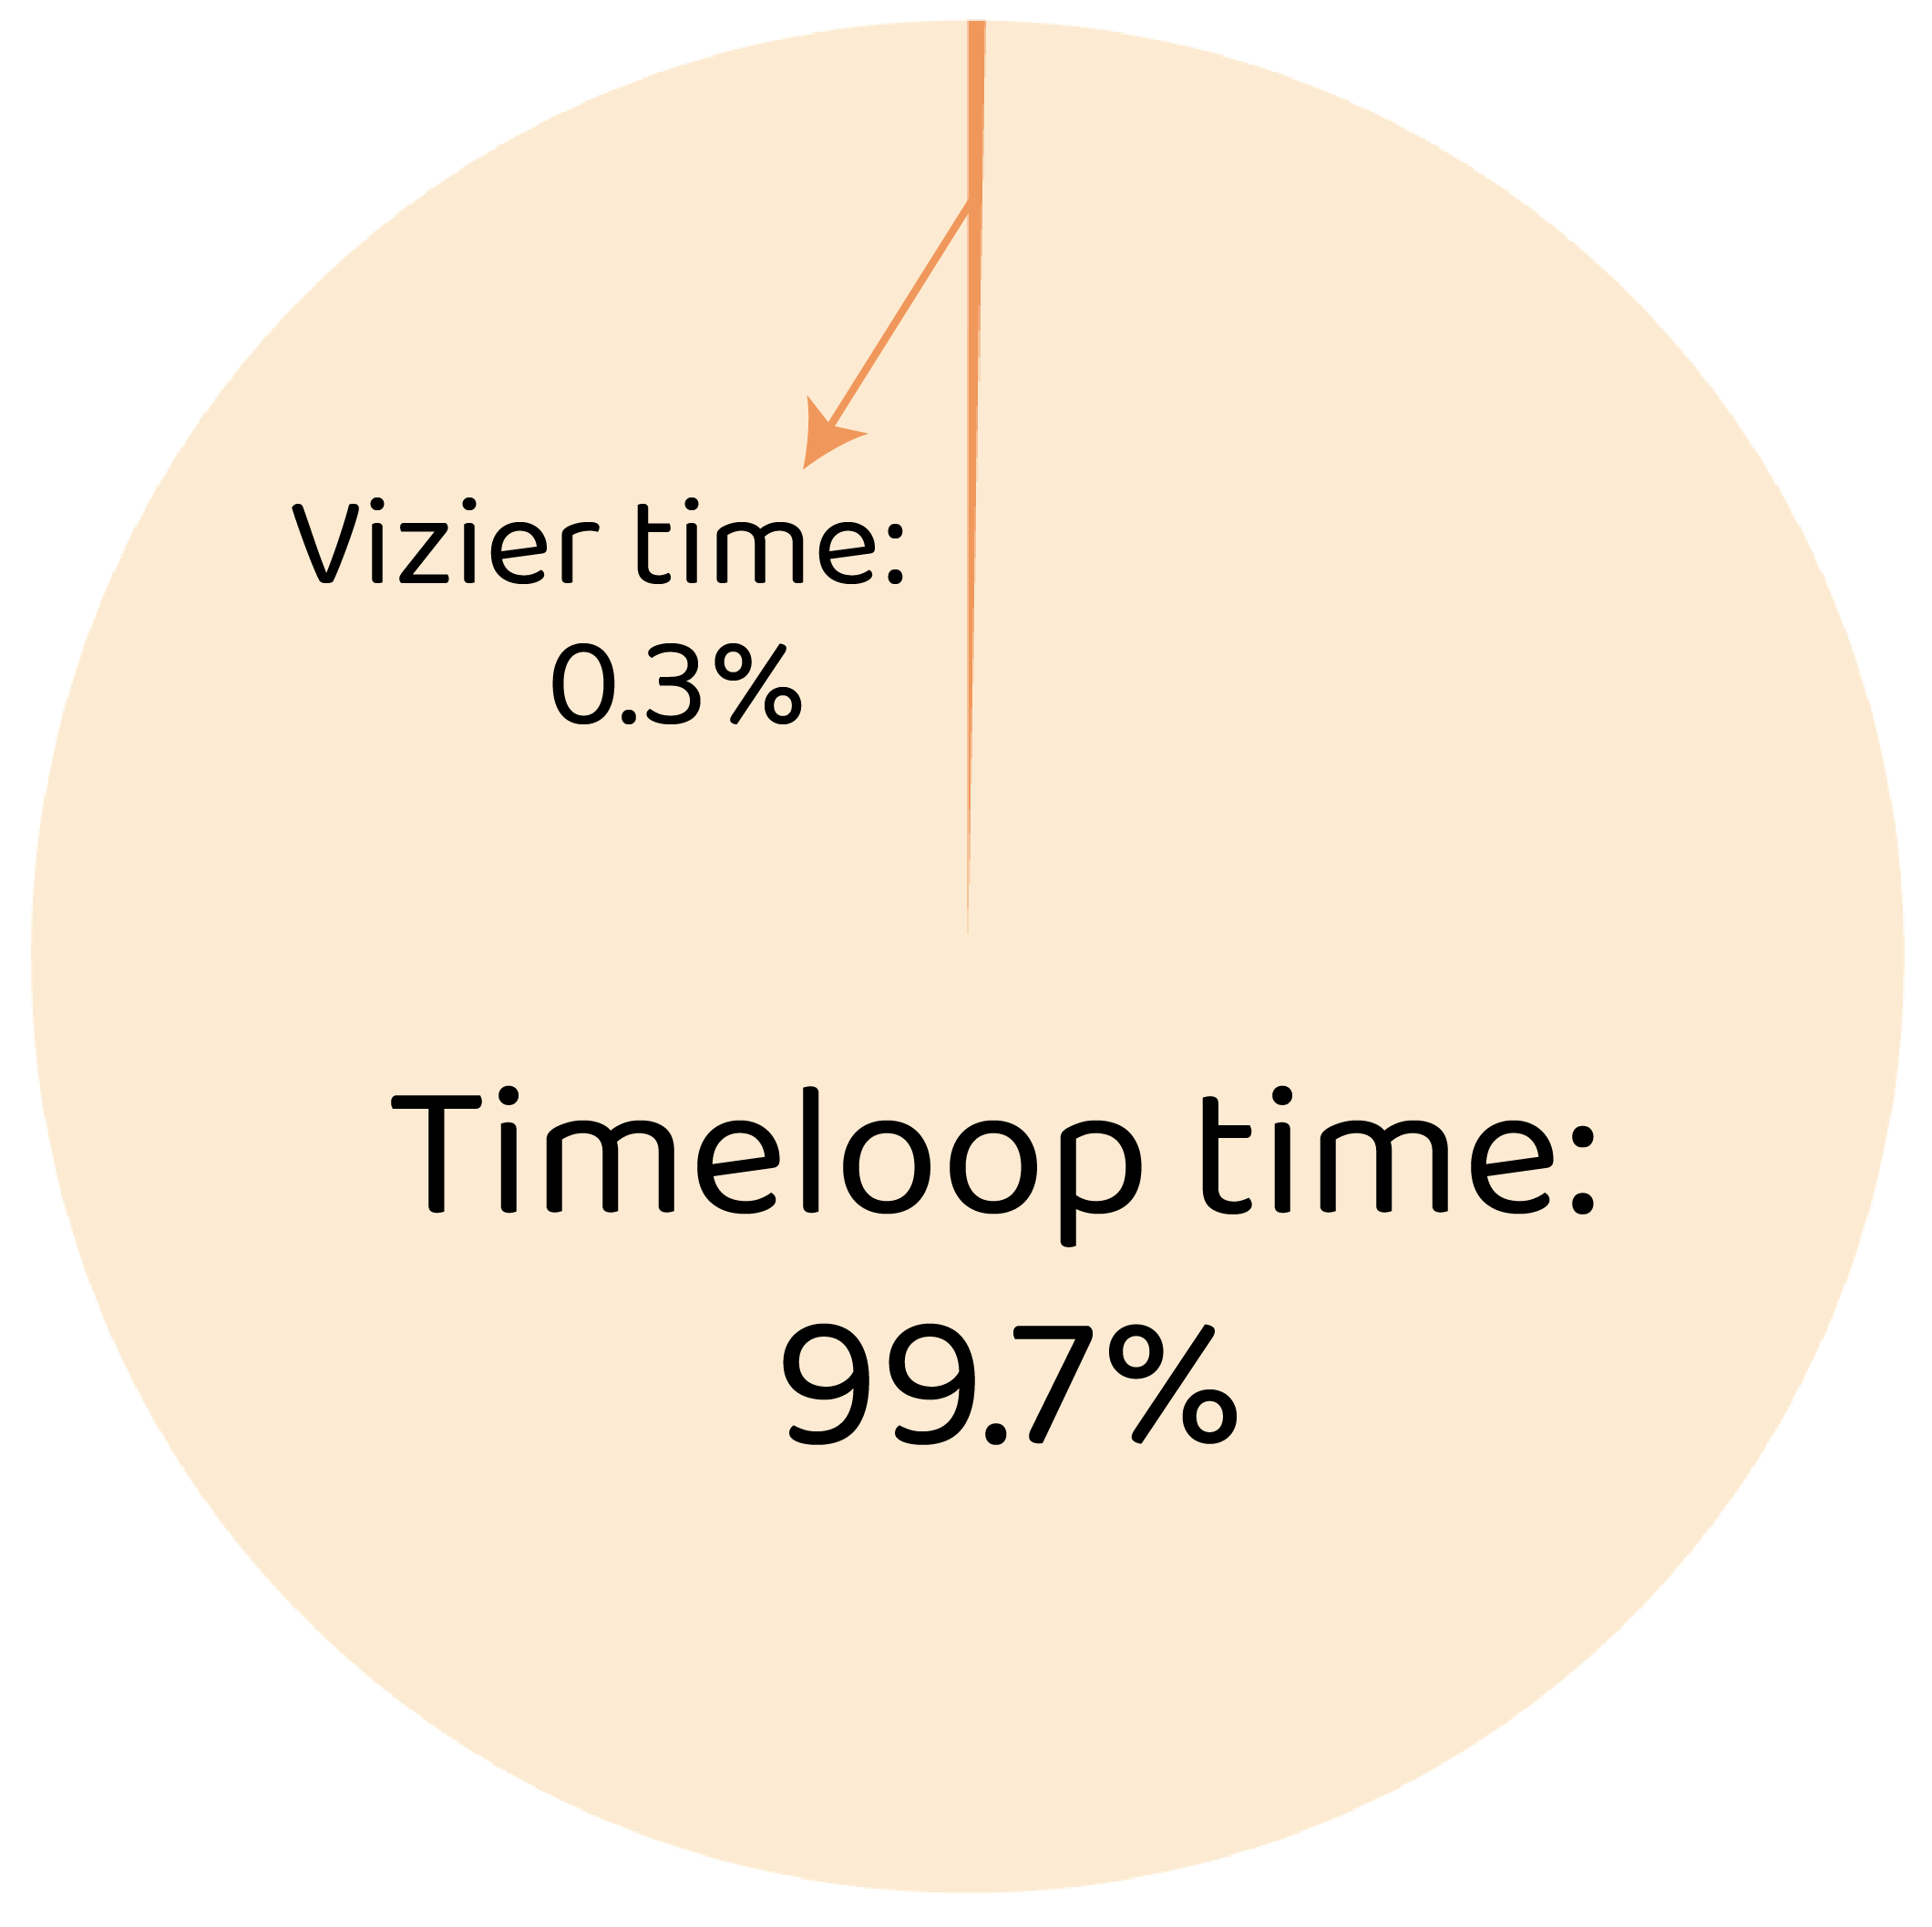
\includegraphics[width=\linewidth]{fig3/timeloop_vs_vizier.png}
    \caption{Per-trial wall-clock breakdown.}
    \label{fig:timeloop-time}
    % \vspace{-10pt}
\end{wrapfigure}
Despite V0's improvements, it inherits the sequential dependence on external tiling tools (e.g., Timeloop) because it lacks a linear expression for non-linear tiling-fusion interactions. As shown in Figure~\ref{fig:timeloop-time}, Timeloop accounts for over 99\% of per-trial latency, creating a prohibitive bottleneck for multi-thousand-trial searches. To resolve this, CHEETAH-V1 internalizes tiling by precomputing Pareto-pruned configurations and encoding them as decision variables. This removes Timeloop from the critical path, collapsing each trial to a single Vizier-proposal and LP-solve step. We start with introducing the preprocessing stage below before presenting the full formulation.

% The limitations of prior work is still inherited in the V0 formulation due to the difficulty of expressing non-linear relationships as linear constraints. Therefore tiling decisions $(\Tmax_i, \Tmin_i, t_i^k)$ are fixed constants provided by additional software, such as Timeloop. A natural question is whether this sequential dependence also creates a \emph{runtime} bottleneck. Figure~\ref{fig:timeloop-time} confirms that it does: across different models, Timeloop scheduling on average accounts for over 99\% of per-trial wall-clock time, while the Vizier proposal and fusion ILP together consume less than 1\% on average. Because the outer loop requires thousands of trials to converge, the cumulative cost of repeated Timeloop invocations dominates the total search budget. This observation motivates a key design choice in CHEETAH-V1: rather than calling Timeloop online during each trial, we precompute a Pareto-pruned set of tiling configurations once (Section~\ref{sec:pareto}) and encode the tiling selection as decision variables \emph{inside} the LP. This eliminates Timeloop from the per-trial critical path entirely, reducing each trial to a single Vizier-proposal$\,\to\,$LP-solve step.

% CHEETAH-V1 captures tiling as a \emph{decision variable} inside the LP, enabling the solver to jointly optimize tiling and fusion. We start with describing our preprocessing stage in Section~\ref{sec:pareto} before presenting the full formulation in Section~\ref{sec::v1}.


\paragraph{Pareto pruning pre-pass.} The raw tiling search space for a $7$-dimensional convolution loop with $3$ memory levels is $\mathcal O(10^7)$ configurations per operation. We reduce this to a tractable Pareto-optimal subset $\mathcal{C}_i$ for each operation $i$ via a pre-pass for (1) L1 feasibility where configurations whose tiled working set exceeds L1 scratchpad capacity $C_{L1}$ are discarded; (2) Pareto optimality where a configuration $c$ is retained only if no other configuration achieves both lower $\Tmax_i(c)$ \emph{and} smaller working-set size in the Global Buffer.

In practice, Pareto pruning reduces $\mathcal O(10^7)$ raw configurations to $|\mathcal{C}_i| \approx 10^2$ to $10^3$ per operation. Timeloop is run once per (operation, configuration) pair, producing the triple $(\Tmin_i(c), \Tmax_i(c), t_i^k(c))$ for each retained configuration $c \in \mathcal{C}_i$. These are precomputed constants: the LP solver makes no Timeloop calls at solve time. Appendix~\ref{app:details} provides more details.

\paragraph{Time-invariant Pareto fronts.}
A key observation is that the Pareto front shape is invariant to memory time: configurations are ranked by compute cycles and working-set bytes, neither of which depends on bandwidth. Changing bandwidth rescales the DRAM access cost $t_i^k(c)$ uniformly. This means the Pareto-pruned configuration sets can be precomputed \emph{once} and reused across all Vizier trials that share the same compute configuration class, amortizing the expensive Timeloop precomputation.

% \subsubsection{The Joint CHEETAH-V1 LP Formulation}\label{sec::v1}

\paragraph{From fixed constants to decision variables.}
V1 brings the tiling choice \emph{inside} the LP by introducing \textbf{tiling selection variables} $y_{i,c} \in [0,1]$, one per Pareto-optimal configuration $c \in \mathcal{C}_i$ from the pre-pass, with the constraint $\sum_c y_{i,c} = 1$ (exactly one configuration is selected per operation). The Timeloop-precomputed constants $\Tmax_i(c)$, $\Tmin_i(c)$, $t_i^k(c)$ now become \emph{per-configuration coefficients} indexed by $c$, so the DRAM savings term becomes $t_i^k(c) \cdot y_{i,c} \cdot p_{\text{assoc}(i,k),\, o(i)}$, a bilinear product that we linearize below.
 
% \paragraph{Linearization via McCormick envelopes.}
% We linearize this product exactly via the classical McCormick substitution. Specifically,  we introduce \textbf{auxiliary variables} $w_{i,c,k} := y_{i,c} \cdot p_{\text{assoc}(i,k),\, o(i)}$ that represent the joint effect of selecting tiling $c$ \emph{and} pinning tensor $k$, constrained by:
% \begin{equation}
% \label{eq:mccormick}
% \begin{aligned}
%     w_{i,c,k} &\leq y_{i,c}, \qquad
%     w_{i,c,k} \leq p_{\text{assoc}(i,k),\, o(i)} \\
%     w_{i,c,k} &\geq y_{i,c} + p_{\text{assoc}(i,k),\, o(i)} - 1, \qquad
%     w_{i,c,k} \geq 0
% \end{aligned}
% \end{equation}
% Since both factors lie in $[0,1]$, these four constraints force $w_{i,c,k} = y_{i,c} \cdot p$ at any integer vertex, requiring no manually tuned constants. Together, $y_{i,c}$ and $w_{i,c,k}$ account for 1.6M of the 2.08M variables in the \Vone~ LP (Table~\ref{tab:v1_scale}). \todo{change to MoE?}

\paragraph{Linearization via McCormick envelopes.}
We linearize this product exactly via the classical McCormick substitution \citep{mccormick1976computability}. For a bilinear term whose factors live in the unit box, the McCormick system is not merely \emph{a} linear relaxation but the convex hull of the product's graph $\{(y,p,w) : w = y\,p,\ 0 \le y,p \le 1\}$: no tighter linear description exists without lifting to additional variables, and it is exact whenever either factor is integral. Relaxation looseness can therefore enter only through fractional $(y,p)$ pairs, a quantity our rounding-and-replay audits measure per workload.
Specifically, we introduce \textbf{auxiliary variables} $w_{i,c,k} := y_{i,c} \cdot p_{\text{assoc}(i,k),\, o(i)}$ that represent the joint effect of selecting tiling $c$ \emph{and} pinning tensor $k$, constrained by:
% \vspace{-4pt}
\begin{equation}
\label{eq:mccormick}
\begin{aligned}
    w_{i,c,k} &\leq y_{i,c}, \qquad
    w_{i,c,k} \leq p_{\text{assoc}(i,k),\, o(i)} \\
    w_{i,c,k} &\geq y_{i,c} + p_{\text{assoc}(i,k),\, o(i)} - 1, \qquad
    w_{i,c,k} \geq 0
\end{aligned}
\end{equation}
Since both factors lie in $[0,1]$, these four constraints force $w_{i,c,k} = y_{i,c} \cdot p$ at any integer vertex, requiring no manually tuned constants.
Geometrically (Figure~\ref{fig:mccormick}), the two upper inequalities are the concave envelope of the bilinear term $w = y\,p$ over the unit box and the two lower ones its convex envelope: the tightest concave over-estimator and convex under-estimator of the product. Because the product is bilinear over a box, these envelopes coincide with the convex hull and are exact at the integer corners, so an integral tile choice is credited with exactly its true DRAM savings, whereas a fractional blend of tiles can be over-credited by up to one quarter of the savings coefficient (at $y = p = \tfrac12$). This over-credit is one of the two mechanisms behind the relaxation gap in V1 and V2, the other being the aggregate roofline row that Section~\ref{sec:v1} disaggregates, and it is exactly what the rounding-and-replay audits measure. Together, $y_{i,c}$ and $w_{i,c,k}$ constitute the majority of V1's decision variables (Table~\ref{tab:v1_scale}).

\begin{figure}[h!]
\centering
\begin{tikzpicture}[x=3.8cm, y=2.8cm, >=stealth, font=\footnotesize]
  % feasible McCormick region on the slice p = 0.2 + 0.6y: a kite with 4 distinct edges
  \fill[red!8] (0,0) -- (0.5,0.5) -- (1,0.8) -- (0.5,0) -- cycle;
  \draw[->] (0,0) -- (1.12,0) node[right] {$y$};
  \draw[->] (0,0) -- (0,1.0) node[above] {$w$};
  \foreach \t in {0,0.5,1} { \draw (\t,0.012) -- (\t,-0.012) node[below] {$\t$}; }
  \foreach \t in {0.5,0.8} { \draw (0.012,\t) -- (-0.012,\t) node[left] {$\t$}; }
  % upper pair: w <= y (slope 1) and w <= p = 0.2 + 0.6y
  \draw[red, dashed, thick] (0,0) -- (0.5,0.5);
  \draw[red, dashed, thick] (0.5,0.5) -- (1,0.8);
  \node[red, above left] at (0.21,0.24) {$w \le y$};
  \node[red, above left, xshift=2pt] at (0.86,0.72) {$w \le p$};
  % lower pair: w >= 0 and w >= y + p - 1 = 1.6y - 0.8
  \draw[red, dashed, thick] (0,0) -- (0.5,0);
  \draw[red, dashed, thick] (0.5,0) -- (1,0.8);
  \node[red, below] at (0.25,-0.05) {$w \ge 0$};
  \node[red, below right] at (0.74,0.30) {$w \ge y + p - 1$};
  % true product along the slice: w = y(0.2 + 0.6y)
  \draw[blue, very thick, domain=0:1, samples=60, smooth] plot (\x, {\x*(0.2+0.6*\x)});
  \node[blue] at (0.67,0.50) {$w = y\,p$};
  % maximal gap at y = p = 1/2
  \draw[<->, gray] (0.5,0.27) -- (0.5,0.48);
  \node[gray, left] at (0.49,0.38) {gap $\tfrac14$};
  % exact at the integer corners
  \fill (0,0) circle (1.4pt);
  \fill (1,0.8) circle (1.4pt);
  \node[above right, yshift=2pt] at (0,0) {exact};
  \node[above, yshift=2pt] at (1,0.8) {exact};
\end{tikzpicture}
\caption{McCormick envelope of the bilinear term $w = y\,p$ on the unit box, drawn along the slice $p = 0.2 + 0.6\,y$ so that all four inequalities of \eqref{eq:mccormick} are distinct lines: the upper pair $w \le y$, $w \le p$ forms the roof and the lower pair $w \ge 0$, $w \ge y + p - 1$ the floor of the shaded feasible region, and the true product (blue) lies inside, touching the envelope only at the integer corners $y \in \{0,1\}$. The largest over-credit is $\tfrac14$, attained at $y = p = \tfrac12$.}
\label{fig:mccormick}
\end{figure}
% \vspace{-4pt}
\paragraph{The Joint CHEETAH-V1 LP Formulation.}
Combining tiling selection, time-indexed placement, rematerialization, and McCormick linearization yields the full V1 program. We do not display it separately: it is the special case of the flagship program \eqref{eq:v1} with the hardware reciprocals $v,u$ pinned to the proposed chip, the CGM one-hot $h_{\mathrm{GM}}$ pinned to its memory, and the tile-dependent families $z^{\mathrm{act}}, z^{W}$ dropped; it in turn contains the fixed-chip program \eqref{eq:v0}, and \eqref{eq:v1} is displayed in full at the end of Section~\ref{sec:v1}.

\paragraph{Tile-dependent residency.}
Extending V1's linearization, V2 introduces two additional McCormick families
for the bilinear products that couple tile choice to on-chip residency:
\begin{equation}
\label{eq:mccormick_v2}
\begin{aligned}
z^{\mathrm{act}}_{e,c,t} \equiv y_{\mathrm{dst}(e),c}\, p_{e,t}: \quad
& z^{\mathrm{act}}_{e,c,t} \leq y_{\mathrm{dst}(e),c}, \quad
  z^{\mathrm{act}}_{e,c,t} \leq p_{e,t}, \\
& z^{\mathrm{act}}_{e,c,t} \geq y_{\mathrm{dst}(e),c} + p_{e,t} - 1, \quad
  z^{\mathrm{act}}_{e,c,t} \geq 0, \\[3pt]
z^{W}_{i,c,t} \equiv y_{i,c}\, p^{W}_{i,t}: \quad
& z^{W}_{i,c,t} \leq y_{i,c}, \quad
  z^{W}_{i,c,t} \leq p^{W}_{i,t}, \\
& z^{W}_{i,c,t} \geq y_{i,c} + p^{W}_{i,t} - 1, \quad
  z^{W}_{i,c,t} \geq 0.
\end{aligned}
\end{equation}
V2 also promotes the CGM size itself to an LP decision.  Let $\{2^k \text{ MiB}
: k = 0, \ldots, K-1\}$ be a discrete size grid and $h_{\mathrm{GM},k} \in [0,1]$
a one-hot selector; the chip's on-chip global-buffer capacity is then
$\sum_{k} 2^{k}\, h_{\mathrm{GM},k}$ bytes.
% \vspace{-4pt}

\paragraph{Hardware sizing inside the same program.}\label{sec:v3}
The rows above optimize the schedule for a \emph{fixed} chip proposed by the
outer loop. CHEETAH-V1 closes the final decoupling in the same program: it
promotes the chip's compute and bandwidth to LP decisions and replaces the
aggregate roofline with its exact convex hull. Fixing the hardware knobs and
collapsing the disaggregated variables recovers the fixed-chip case exactly, so
this single formulation subsumes CHEETAH-V0 and is our flagship program.

\paragraph{Hardware as decision variables.}
Alongside the one-hot CGM selector $h_{\mathrm{GM},k}$, the flagship program
\eqref{eq:v1} sizes the MAC array
and DRAM bandwidth \emph{inside} the program. Writing the reference-normalized
reciprocals $v = M_{\mathrm{ref}}/\mathrm{MACs}$ and
$u = \mathrm{BW_{ref}}/\mathrm{BW}$ (so a tile's compute time is $\Tmin_i(c)\,v$
and its memory time is $\Tmax_i(c)\,u$), the chip must respect the same-silicon
area and power envelopes
\begin{equation}
\kappa_{\mathrm{MAC}}\,\mathrm{MACs}
 + \kappa_{\mathrm{SRAM}}\!\sum_{k} 2^{k} h_{\mathrm{GM},k}
 + \kappa_{\mathrm{BW}}\,\mathrm{BW} \;\le\; A_{\mathrm{cap}},
\qquad
\pi_{\mathrm{MAC}}\,\mathrm{MACs} \;\le\; P_{\mathrm{cap}} .
\label{eq:v3_caps}
\end{equation}
The reciprocals are convex epigraphs, and the program is a linear program.
Bandwidth \emph{is} a finite menu: $\mathrm{BW}$ is a one-hot selection
$\nu_\ell$ over the gate-feasible legal points $\mathrm{BW}_\ell$
($8$ of the $12$ catalogue points on DeepSeek-V3 pass the pin gate
$\mathrm{BW}/0.8\le 4096$ pins), so
$u=1/\mathrm{BW}=\sum_\ell \nu_\ell/\mathrm{BW}_\ell$ is exact at integral
$\nu$ and the LP relaxation of the menu is a valid lower bound. The compute
reciprocal $v \ge 1/m$ is bracketed by tangent rows on a geometric grid of $m$
(a valid relaxation, hence a certified lower bound) and by chord rows on the
same grid (an inner approximation); with 89 grid rows each envelope is within
$10^{-3}$ of $1/m$, so the bracket is at most $2\times10^{-3}$ wide, and no
auxiliary variable is needed. Every product of a
menu selector with a continuous quantity is written as its convex hull
(disaggregated copies with a linking equality), which is exact at integral
selectors; McCormick envelopes are used only in that hull form. The chord
(inner) LP yields an achievable design only once every menu selector is pinned
to an integral value and the pinned solution passes an exact-lift check
(reciprocals and products set to their true values, every original row
re-verified); with relaxed selectors it is neither a lower nor an upper bound,
so every ``exact'' below means exact at integral selectors. This internalizes the hardware proposal the outer loop previously
made, so a single solve sizes chip \emph{and} schedule jointly under a hard
area/TDP budget.

\paragraph{Disaggregated perspective epigraph.}
The aggregate roofline row
$T_i \ge \max\!\big(\sum_c \Tmin_i(c)\,y_{i,c}\,v,\; \sum_c (\Tmax_i(c){-}\mathrm{save})\,y_{i,c}\,u\big)$,
the form used before the per-tile split below,
is loose once $y$ is fractional: it lets the solver blend a compute-bound tile
against a bandwidth-bound tile and hide \emph{both} bottlenecks
(the source of a large relaxation gap on weight-heavy models). The flagship
program \eqref{eq:v1} replaces it
with the disaggregated perspective form
\begin{equation}
\begin{aligned}
&\textstyle\sum_c v_{i,c}=v,\quad \sum_c u_{i,c}=u;\qquad
 \underline v\,y_{i,c}\le v_{i,c}\le \overline v\,y_{i,c},\quad
 \underline u\,y_{i,c}\le u_{i,c}\le \overline u\,y_{i,c};\\[2pt]
&\tau_{i,c}\ge \Tmin_i(c)\,v_{i,c},\quad
 \tau_{i,c}\ge \big(\Tmax_i(c)-\mathrm{save}_{i,c}\big)\,u_{i,c},\quad
 T_i\ge \textstyle\sum_c \tau_{i,c},
\end{aligned}
\label{eq:v3_epigraph}
\end{equation}
which is the closed convex hull of the per-op ``pick one tile, pay its roofline
maximum'' disjunction: it enforces $T_i \ge \sum_c \max(\cdot,\cdot)$ rather than
the weaker $\max(\sum,\sum)$, tightening the certified lower bound at no cost to
feasibility and preserving exactness at every integer vertex.

\paragraph{Certified column generation.}
The Pareto tile set $\mathcal C_i$ is a column \emph{pool}: a candidate
tiling/mapping enters only when its reduced cost against the converged LP dual
variables is negative. The native mapper (or the LLM-Architect outer loop,
which reads exactly these Lagrangian duals) can therefore \emph{propose}
columns while the LP \emph{scores and certifies} them. The oracle can reshape
where the search looks; it can never weaken the optimality certificate. This is
the mechanism that makes ``the LLM proposes, the solver certifies'' rigorous,
and it is what the outer loop of the next subsection exploits.

\paragraph{The joint CHEETAH-V1 LP formulation.}
Collecting the pieces, the full V1 program takes the fixed-chip rows above with the aggregate
roofline row replaced by the disaggregated perspective epigraph, the reciprocals
$v,u$ and the memory one-hot promoted to decisions under the same-silicon caps,
and one further hull family $X_{i,c,\ell}$, the bandwidth-menu copies of the
memory-time numerator $X_{i,c}=\Tmax_i(c)\,y_{i,c}-\sum_k t_i^k(c)\,w_{i,c,k}$,
so that the DRAM savings scale with bandwidth exactly at integral $\nu$. Writing $m = \mathrm{MACs}/M_{\mathrm{ref}}$ and
$\beta = \mathrm{BW}/\mathrm{BW_{ref}}$, the program is \eqref{eq:v1}.
The CHEETAH-V1 LP formulation is:
\begin{equation}
\begin{aligned}
\min \quad & \sum_{i \in \mathcal{N}} T_i \;+\;
             \sum_{i \in \mathcal{N}} \sum_{t \in \mathcal{T}} c_i^{\text{remat}}\, r_{i,t}
             \;+\; \varepsilon_{\mathrm{CGM}} \sum_{k=0}^{K-1} k \, h_{\mathrm{GM},k} \\[3pt]
\text{s.t.} \quad
& \sum_{c \in \mathcal{C}_i} y_{i,c} = 1 \;\;\forall\, i, \qquad
  \sum_{k=0}^{K-1} h_{\mathrm{GM},k} = 1 \\[3pt]
& v \;\geq\; \tfrac{2}{m_j} - \tfrac{m}{m_j^{2}} \quad \forall\, j \in \mathcal{J}
  \quad\text{(tangent rows; chord rows for the inner LP)} \\[3pt]
& \beta = \textstyle\sum_{\ell} \nu_\ell\, \beta_\ell, \qquad
  u = \textstyle\sum_{\ell} \nu_\ell/\beta_\ell, \qquad
  \textstyle\sum_{\ell} \nu_\ell = 1 \quad\text{(bandwidth menu)} \\[3pt]
& \kappa_{\mathrm{MAC}}\,\mathrm{MACs} + \kappa_{\mathrm{SRAM}}\!\sum_{k} 2^{k} h_{\mathrm{GM},k}
  + \kappa_{\mathrm{BW}}\,\mathrm{BW} \leq A_{\mathrm{cap}}, \qquad
  \pi_{\mathrm{MAC}}\,\mathrm{MACs} \leq P_{\mathrm{cap}} \\[3pt]
& \sum_{c \in \mathcal{C}_i} v_{i,c} = v, \qquad \sum_{c \in \mathcal{C}_i} u_{i,c} = u
  \quad \forall\, i \\[3pt]
& \underline v\, y_{i,c} \leq v_{i,c} \leq \overline v\, y_{i,c}, \qquad
  \underline u\, y_{i,c} \leq u_{i,c} \leq \overline u\, y_{i,c}
  \quad \forall\, i, c \\[3pt]
& \tau_{i,c} \geq \Tmin_i(c)\, v_{i,c}, \qquad
  \tau_{i,c} \geq \textstyle\sum_{\ell} X_{i,c,\ell}/\beta_\ell, \qquad
  T_i \geq \sum_{c \in \mathcal{C}_i} \tau_{i,c} \quad \forall\, i, c \\[3pt]
& \text{Envelopes~\eqref{eq:mccormick} for } w_{i,c,k};\;
  X_{i,c} = \Tmax_i(c)\,y_{i,c} - \textstyle\sum_k t_i^k(c)\,w_{i,c,k} = \textstyle\sum_{\ell} X_{i,c,\ell}
  \quad \forall\, i, c \\[3pt]
& \underline X_{i,c}\,\nu_\ell \le X_{i,c,\ell} \le \Tmax_i(c)\,\nu_\ell
  \quad \forall\, i, c, \ell \\[3pt]
& 
  \text{\eqref{eq:mccormick_v2} for } z^{\mathrm{act}}_{e,c,t}, z^{W}_{i,c,t} \\[3pt]
& \sum_{e \in \mathcal{E}_{\mathrm{live}}(t)} \sum_{c}
    d^{\mathrm{act}}_{e,c}\, z^{\mathrm{act}}_{e,c,t}
  + \sum_{i} \sum_{c} d^{W}_{i,c}\, z^{W}_{i,c,t}
  \leq \sum_{k=0}^{K-1} 2^{k}\, h_{\mathrm{GM},k}
  \quad \forall\, t \\[3pt]
& p_{e,t} \leq p_{e,t-1} + r_{\text{src}(e),\, t} \;\;\forall\, e,\, t > o(\text{src}(e)); \qquad
  p_{i,t}^W \leq p_{i,t-1}^W \;\;\forall\, i,\, t > o(i) \\[3pt]
& r_{i,t} = 0 \;\;\forall\, t \leq o(i); \qquad
  r_{i,t} \leq \min\!\big(p_{e,t},\, p_{i,t}^W\big)
  \;\;\forall\, e \in \text{in}(i),\, t > o(i) \\[3pt]
& T_i,\, \tau_{i,c},\, v_{i,c},\, u_{i,c} \geq 0; \quad
  y, p, p^W, r, w, z, h_{\mathrm{GM}}, \nu \in [0,1]; \quad
  v \in [\underline v, \overline v],\; u \in [\underline u, \overline u]
\end{aligned}
\tag{V1}\label{eq:v1}
\end{equation}

Here $\underline X_{i,c}=\min\{0,\,\Tmax_i(c)-\sum_k t_i^k(c)\}$: in the
measured tile caches the per-tensor byte terms can exceed $\Tmax_i(c)$, so the
numerator box is not sign-restricted, and the bandwidth-menu rows
($X_{i,c,\ell}$, $\nu_\ell$) are exact at integral $\nu$.
Pinning $(v,u,h_{\mathrm{GM}})$ to a proposed chip makes the cap, tangent, and
link rows inert, turns the menu copies $X_{i,c,\ell}$ into the constant multiple
$X_{i,c}/\beta$, and leaves
\eqref{eq:v1} up to the tightening of Corollary~\ref{cor:v3_hull}; this is the
precise sense in which the flagship program subsumes V0. When an achievable
certified sub-problem is required, the compute tangent rows are replaced by the
chord rows with every menu selector pinned (the inner LP), whose solution is a
design once the exact-lift check passes; bandwidth is already a menu and needs no
replacement. This is the form used by the column-generation oracle.

\subsection{The Comprehensive CHEETAH-V1: Serving-Regime Co-Design Decisions}\label{sec:v3_levers}
Program~\eqref{eq:v1} sizes compute, bandwidth, and on-chip memory jointly with
the schedule. The memory-bound decode regime of LLM, MoE, and diffusion serving
admits four further decisions, each of which reduces the bytes moved or sets a
hardware capacity, hence is a linear (or McCormick-linearizable) addition to
the flagship program \eqref{eq:v1} rather than an outer-loop guess. We fold them in below. Every added block is
\emph{inert when pinned}: fixing its selector to a baseline policy leaves
\eqref{eq:v1}, and with it the V0 and V1 chain, exactly intact, so the subsumption
property is preserved. Decisions that only rescale coefficients (the decode batch
$N$, the speculative-decode width $K$) enter as workload parameters that reshape
the per-op dimensions and thus arithmetic intensity, and the flagship program
\eqref{eq:v1} evaluates any $(N,K)$ without deciding them; genuinely discrete or non-convex choices (draft
model, eviction policy, denoising-step schedule) remain columns the outer loop
proposes and the LP evaluates against its duals. Accuracy is never linearized: each
precision menu below is restricted to configurations the quantization literature
certifies as lossless-enough.

\paragraph{Precision as a decision (per phase, per expert).}
Let $\mathcal{Q}$ be an accuracy-vetted precision menu, each point $\rho$
carrying weight-, activation-, and KV-bit fractions $(b^W_\rho,b^A_\rho,
b^{\mathrm{KV}}_\rho)$ relative to the 8-bit baseline. We write a menu entry as
$\mathrm{W}w\mathrm{A}a$, meaning $w$-bit weights and $a$-bit activations, with a
trailing $/\mathrm{KV}k$ when the KV cache is additionally held at $k$ bits. The
menu used here is
\[
  \rho \in \{\;
  \underbrace{\mathrm{W8A8}}_{\text{8-bit weights, 8-bit activations}},\;
  \underbrace{\mathrm{W4A8}}_{\text{4-bit weights, 8-bit activations}},\;
  \underbrace{\mathrm{W4A8/KV4}}_{\text{as W4A8, plus a 4-bit KV cache}},\;
  \underbrace{\mathrm{W4A16}}_{\text{4-bit weights, 16-bit activations}}
  \;\},
\]
each admissible under AWQ, GPTQ and KVQuant
\citep{lin2024awq,frantar2023gptq,hooper2024kvquant}. Narrower weights reduce the
bytes a decode step must stream, which is the dominant cost; narrower activations
additionally reduce multiplier switching energy, and \cref{sec:energy_coeff}
reports the measured saving for each entry. Per phase
$\phi \in \{\mathrm{pre},\mathrm{dec}\}$ a one-hot selector chooses the operating
precision, inducing byte-scales:
\begin{equation}
\sum_{\rho} q_{\phi,\rho} = 1,\qquad
s^{W}_\phi = \sum_\rho b^W_\rho\, q_{\phi,\rho},\qquad
s^{\mathrm{KV}}_\phi = \sum_\rho b^{\mathrm{KV}}_\rho\, q_{\phi,\rho},\qquad
q_{\phi,\rho}\in\{0,1\}.
\label{eq:v3_prec}
\end{equation}
The weight and KV byte footprints $d^{W}_{i,c}$ and $d^{\mathrm{KV}}$ in the
capacity row and the DRAM-savings term are replaced by $s^{W}_{\phi}d^{W}_{i,c}$
and $s^{\mathrm{KV}}_{\phi}d^{\mathrm{KV}}$; the resulting selector-times-variable
products are written as hull disaggregations of the per-step byte aggregates
over the precision menu (exact at integral $q$). For a mixture-of-experts layer the phase index is
refined to an \emph{expert} index: each expert $e$ carries its own one-hot
$q_{e,\rho}$ and byte-scale $s^{W}_e=\sum_\rho b^W_\rho q_{e,\rho}$, so the solver
may place the lowest-bit points on the hottest experts, where weight-reload
traffic dominates.

\paragraph{Energy-aware same-silicon cap.}
Precision helps under a fixed power budget only if bandwidth actually costs
power, so the cap of~\eqref{eq:v3_caps} is extended to charge DRAM traffic at
$\pi_{\mathrm{bit}}$ joules per bit:
\begin{equation}
\pi_{\mathrm{MAC}}\,\mathrm{MACs} \;+\; \pi_{\mathrm{bit}}\, \varrho_{\mathrm{DRAM}}
\;\le\; P_{\mathrm{cap}},
\qquad
\varrho_{\mathrm{DRAM}} = \sum_{\text{class}\,\in\,\{W,A,\mathrm{KV}\}}
   s^{\text{class}}_{\phi}\,\beta_{\text{class}} ,
\label{eq:v3_power}
\end{equation}
where $\varrho_{\mathrm{DRAM}}$ is the precision-scaled DRAM byte-rate over the
weight, activation, and KV classes; each $\beta_{\text{class}}$ is a workload
constant (the bytes of that class streamed at the reference operating point),
so the row is linear in the precision selectors. Setting $\pi_{\mathrm{bit}}=0$ recovers
\eqref{eq:v3_caps}; a positive $\pi_{\mathrm{bit}}$ is precisely what makes
provisioned bandwidth ``cost power'' in the certified program, so the
byte-reducing decisions (precision, KV budget, expert residency) relax the same cap
that raw bandwidth tightens.

\paragraph{MoE expert residency (HBM pinning).}
Let $C_{\mathrm{HBM}}$ be the fast-memory capacity, a hardware decision entering
the area cap, and let $f_e\in[0,1]$ be expert $e$'s measured routing frequency (a
workload statistic). A pin variable $g_e$ is the resident fraction of expert
$e$'s weights: residency is knapsack-constrained, and an offloaded expert pays a
per-visit reload:
\begin{equation}
\sum_{e} g_e\, s^{W}_e\, W_e \;\le\; C_{\mathrm{HBM}},
\qquad
\Delta^{\mathrm{moe}}_{\mathrm{dram}} = \sum_{e} f_e\,(1-g_e)\, s^{W}_e\, W_e,
\qquad g_e \in [0,1],
\label{eq:v3_expres}
\end{equation}
with $W_e$ the expert weight bytes and $\Delta^{\mathrm{moe}}_{\mathrm{dram}}$ the
expert-reload traffic added to the decode memory term. Pinning the hottest
experts removes their reload; the dual variable $\lambda_{\mathrm{HBM}}$ of the
capacity row is the marginal value of fast memory the outer loop reads when
sizing $C_{\mathrm{HBM}}$.

\paragraph{KV budget (eviction as a resource cap).}
A retained-cache budget $B^{\mathrm{KV}} \in [B_{\min},L_{\mathrm{ctx}}]$ replaces
the growing context length in the attention-input traffic, with $B_{\min}$ the
quality floor of the eviction method (external). With per-token KV footprint
$d^{\mathrm{KV}}$ and an on-chip residency indicator $\sigma_{\mathrm{KV}}\in
\{0,1\}$, the budget is disaggregated over the joint one-hot $\pi_{\rho,s}$ of
decode precision $\rho$ and residency branch $s\in\{\mathrm{on},\mathrm{off}\}$
(with $\sum_{\rho,s}\pi_{\rho,s}=1$, $\sum_s\pi_{\rho,s}=q_{\mathrm{dec},\rho}$,
$\sum_\rho\pi_{\rho,\mathrm{on}}=\sigma_{\mathrm{KV}}$),
\begin{equation}
\begin{aligned}
&B^{\mathrm{KV}}=\textstyle\sum_{\rho,s}B_{\rho,s},\qquad
B_{\min}\,\pi_{\rho,s}\le B_{\rho,s}\le L_{\mathrm{ctx}}\,\pi_{\rho,s},\\[2pt]
&\Delta^{\mathrm{KV}}_{\mathrm{dram}} =
   d^{\mathrm{KV}}\textstyle\sum_\rho b^{\mathrm{KV}}_\rho\, B_{\rho,\mathrm{off}},
\qquad
d^{\mathrm{KV}}\textstyle\sum_\rho b^{\mathrm{KV}}_\rho\, B_{\rho,\mathrm{on}}
   \;\le\; \textstyle\sum_k 2^k h_{\mathrm{GM},k},
\end{aligned}
\label{eq:v3_kvbudget}
\end{equation}
a two-branch hull with no big-$M$, exact at integral $(q,\sigma_{\mathrm{KV}})$,
so that a small enough budget on the on-chip branch ($\sigma_{\mathrm{KV}}=1$)
lets the KV read be served on chip and leave the DRAM term, coupling the
eviction budget directly to CGM sizing through $\lambda_{\mathrm{CGM}}$.

\paragraph{Diffusion cross-step reuse (DeepCache).}
For an $S$-step denoiser, a per-block reuse variable $\chi_b\in[0,1]$ caches block
$b$'s slow-changing feature map across a window of $W$ steps instead of
recomputing it each step:
\begin{equation}
\widehat{\mathrm{cost}}_b = \big(1 - \chi_b(1 - \tfrac1W)\big)\,\mathrm{cost}_b,
\qquad
\sum_b \chi_b\, F_b \;\le\; \textstyle\sum_k 2^k h_{\mathrm{GM},k},
\label{eq:v3_deepcache}
\end{equation}
where $\mathrm{cost}_b$ is block $b$'s per-step compute and feature traffic, $F_b$
its cached-feature footprint, and the window $W$ and cacheable set are workload
statistics. This gives the otherwise fusion-inert diffusion workload a genuine
cross-step memory decision, the temporal analog of the KV cache.

The remaining decisions are drawn from production serving and kernel systems
(vLLM, SGLang, ThunderKittens, TensorRT-LLM); each enriches the \emph{software}
side of the model and, crucially, ties it more tightly to a \emph{hardware} knob,
so the LP models how the chip and the kernel react to one another.

\paragraph{Prefill--decode interleaving.}
Serving co-schedules compute-bound prefill chunks with memory-bound decode steps;
because their bottlenecks are complementary, an interleaved window fills both
rooflines at once. An interleave fraction $\theta\in[0,\theta_{\max}]$ (bounded by
the prefill backlog and a per-token latency SLA) folds prefill into the decode
window, and the additive $T^{\mathrm{pre}}+N\,T^{\mathrm{dec}}$ is replaced by a
mixed-window epigraph,
\begin{equation}
T_{\mathrm{serve}} \ge \theta\,C^{\mathrm{pre}} + N\,C^{\mathrm{dec}},
\qquad
T_{\mathrm{serve}} \ge \theta\,M^{\mathrm{pre}} + N\,M^{\mathrm{dec}},
\label{eq:v3_interleave}
\end{equation}
with $C^{\mathrm{ph}}$ the lifted compute streams (linear in the per-branch
copies of $v$), $M^{\mathrm{ph}}$ the bandwidth-menu memory streams (linear in
the copies $X_{i,c,\ell}$), and $\theta$ a scheduler constant rather than a
decision, so $T_{\mathrm{serve}}\ge\max(\cdot,\cdot)$ over the combined stream and the optimal
$(v,u)$ ratio now tracks the \emph{combined} arithmetic intensity rather than
either phase alone \citep{kwon2023vllm}.

\paragraph{Load-engine vs.\ compute-worker datapath split.}
Following the load/store-vs-compute worker split of tile kernels
\citep{spector2024thunderkittens}, the die is partitioned between MAC units and
data-movement (DMA/async-copy) engines, and the provisioned bandwidth is
realizable only if enough load engines back it. Adding a load-engine throughput
$B_{\mathrm{LD}}$ (area cost $\kappa_{\mathrm{LD}}$) to the area cap,
\begin{equation}
\kappa_{\mathrm{MAC}}\mathrm{MACs} + \kappa_{\mathrm{LD}}B_{\mathrm{LD}}
 + \kappa_{\mathrm{SRAM}}\!\sum_k 2^k h_{\mathrm{GM},k} + \kappa_{\mathrm{BW}}\mathrm{BW}
 \le A_{\mathrm{cap}},
\qquad
\mathrm{BW}_{\mathrm{eff}} \le \mathrm{BW},\;\; \mathrm{BW}_{\mathrm{eff}} \le B_{\mathrm{LD}},
\label{eq:v3_datapath}
\end{equation}
and the perspective reciprocal reads $u=\mathrm{BW_{ref}}/\mathrm{BW_{eff}}$: a
memory-bound decode buys load engines ($\lambda_{\mathrm{LD}}$ large), a
compute-bound prefill buys MACs, a split the solver makes per phase.

\paragraph{Prefix and KV cache reuse (RadixAttention).}
Shared prompt prefixes (system prompts, few-shot exemplars, chat history,
repeated images) let requests reuse cached KV, cutting both prefill compute and
KV traffic \citep{zheng2024sglang,kwon2023vllm}. With a cache capacity
$C_{\mathrm{cache}}$ (a hardware decision in the area cap) and a saturating
hit-rate profile $\eta_s\in[0,1)$ measured under cache-aware
(longest-shared-prefix-first) scheduling for the workload's sharing structure, a
one-hot over cache sizes $s\in\mathcal{S}$ scales the reused terms:
\begin{equation}
\sum_s \rho_s = 1,\quad \eta_{\mathrm{hit}} = \sum_s \eta_s\,\rho_s,\quad
\widehat C^{\mathrm{pre}} = (1-\eta_{\mathrm{hit}})\,C^{\mathrm{pre}},\quad
\widehat M^{\mathrm{pre}} = (1-\eta_{\mathrm{hit}})\,M^{\mathrm{pre}},
\label{eq:v3_radix}
\end{equation}
so the solver trades cache area against the prefill recompute and traffic it
removes. The credit applies to the prefill streams only: the decode KV traffic
$\Delta^{\mathrm{KV}}_{\mathrm{dram}}$ is not credited, because a shared prefix
is re-read at every decode step whether or not it was cached at prefill (the
convention of \cref{sec:decode_decomp}). The $\eta_{\mathrm{hit}}\,C^{\mathrm{pre}}$
and $\eta_{\mathrm{hit}}\,M^{\mathrm{pre}}$ products are exact by disaggregating
the prefill streams over the cache-size menu $\rho_s$; the LP relaxation of that
menu is the chord hypograph of the measured hit-rate curve.

\paragraph{Array shape and native tile granularity.}
Fixing MAC \emph{count} leaves the array \emph{shape} free, and utilization is
acutely shape-dependent (a square array idles on skinny decode GEMVs and
depthwise convs, the very cause of the mapper underutilization behind our
analytic compute floor). A one-hot $\alpha_a$ over aspect ratios / native-MMA
tiles $a\in\mathcal{A}$ ($16{\times}16$, WGMMA, TCGEN05) carries a precomputed
per-op utilization $\eta_{i,a}\in(0,1]$; disaggregating $v_{i,c}$ over $a$ as in
the perspective epigraph,
\begin{equation}
\textstyle\sum_a v^{a}_{i,c} = v_{i,c},\quad
0 \le v^{a}_{i,c} \le \overline v\,\alpha_a,\quad
\tau_{i,c} \ge \sum_a \tfrac{\Tmin_i(c)}{\eta_{i,a}}\, v^{a}_{i,c},
\label{eq:v3_arrayshape}
\end{equation}
which co-designs the array to the workload's matmul shapes and directly serves
LLM/MoE decode GEMVs and EfficientNet depthwise convs
\citep{spector2024thunderkittens}. The lower bound $\underline v\,y_{i,c}\le
v_{i,c}$ lives on the tile selector in \eqref{eq:v3_epigraph} and is inherited
by the copies through the linking sum, not placed on the aspect copies: since
$\sum_a\alpha_a=1$, a positive lower bound on every copy would force
$v_{i,c}\ge\underline v$ on every non-selected tile and make every integral tile
choice infeasible (this was found and fixed in the implementation on
2026-09-20). The DVFS copies $v^{f}_{i,c}$ of \eqref{eq:v3_dvfs} carry the same
one-sided bounds, $\sum_f v^{f}_{i,c}=v_{i,c}$ and $0\le v^{f}_{i,c}\le
\overline v\,\phi_{\mathrm{ph},f}$.

\paragraph{Per-phase clock and voltage (DVFS).}
Compute-bound prefill benefits from a high clock; memory-bound decode does not, so
per-phase frequency is a decision. A per-phase one-hot $\phi_{\mathrm{ph},f}$ over
a frequency menu (throughput scale $\gamma_f$, power factor $\pi_f/\pi_0$) scales
the phase compute time and enters the power cap:
\begin{equation}
\sum_f \phi_{\mathrm{ph},f}=1,\qquad
\tau^{\mathrm{ph}}_{i,c} \ge \sum_f \tfrac{\Tmin_i(c)}{\gamma_f}\,v^{f}_{i,c},\qquad
\pi_{\mathrm{MAC}}\mathrm{MACs}\!\sum_f\!\tfrac{\pi_f}{\pi_0}\phi_{\mathrm{dec},f}
 + \pi_{\mathrm{bit}}\varrho_{\mathrm{DRAM}} \le P_{\mathrm{cap}},
\label{eq:v3_dvfs}
\end{equation}
so the chip runs fast in prefill and slow in decode, freeing power for bandwidth
in the phase where compute is idle (the $\mathrm{MACs}\cdot\phi$ term is the hull
$\mathrm{MACs}=\sum_f \mathrm{MACs}_f$, $M_{\min}\phi_f\le\mathrm{MACs}_f\le
M_{\max}\phi_f$, exact at integral $\phi$).

\paragraph{Constrained and speculative decoding (parameters).}
Constrained decoding over a compressed grammar FSM \citep{zheng2024sglang} and
speculative/draft verification emit $K>1$ tokens per forward pass on deterministic
or accepted spans, raising decode arithmetic intensity toward the compute-bound
regime. Like the batch $N$, the effective width $K$ (and the deterministic or
accepted fraction) is a \emph{workload parameter} the program evaluates, not a
decision; the draft model and grammar remain outer-loop inputs.

\paragraph{The comprehensive program and its constraint signals.}
The comprehensive CHEETAH-V1 program is \eqref{eq:v1} augmented with the
precision, capacity, datapath, and scheduling families
\eqref{eq:v3_prec}--\eqref{eq:v3_dvfs}: the interleaved perspective epigraph now
reads the precision-scaled and cache-reduced bytes, the reload/eviction deltas
$\Delta^{\mathrm{moe}}_{\mathrm{dram}}+\Delta^{\mathrm{KV}}_{\mathrm{dram}}$,
and the shape-, frequency-, and load-engine-dependent compute in place of the
fixed footprints. Because every block is inert under a pinned policy, the
subsumption chain
\eqref{eq:v0}$\subseteq$\eqref{eq:v1}$\subseteq$(comprehensive program) holds by
construction. Its converged duals are exactly the resource-dual vector the
LLM-Architect outer loop consumes: $\lambda_{\mathrm{BW}}$ (large in decode)
values a GB/s, $\lambda_{\mathrm{MAC}}\!\approx\!0$ in decode makes added
multipliers visibly worthless (the anti-gaming property as a certificate, not a
claim), and $\lambda_{\mathrm{HBM}},\lambda_{\mathrm{CGM}},\lambda_{\mathrm{LD}},
\lambda_{\mathrm{cache}}$ value capacity for expert pinning, KV residency, load
engines, and prefix reuse. The outer loop then proposes only the genuinely
discrete and non-convex axes (interconnect radix, HBM-stack count, array aspect
ratio, whether to spend area on low-bit MAC units, draft model, denoising-step
schedule) as columns; the LP evaluates each by reduced cost and the same-silicon
caps make inflation infeasible, so the search is a dual-steered, certified column
generation rather than a blind sweep.

% \begin{equation}
% \begin{aligned}
% \min \quad & \sum_{i \in \mathcal{N}} T_i + \sum_{i \in \mathcal{N}} \sum_{t \in \mathcal{T}} c_i^{\text{remat}} \, r_{i,t} \\[4pt]
% \text{s.t.} \quad
% & \sum_{c \in \mathcal{C}_i} y_{i,c} = 1 & \forall\, i \in \mathcal{N} \\[3pt]
% & T_i \geq \max\!\left(\sum_{c \in \mathcal{C}_i} \Tmin_i(c)\, y_{i,c},\;\; \sum_{c \in \mathcal{C}_i} \Tmax_i(c)\, y_{i,c} - \sum_{c \in \mathcal{C}_i} \sum_{k} t_i^k(c)\, w_{i,c,k}\right) & \forall\, i \in \mathcal{N} \\[3pt]
% & w_{i,c,k} \leq y_{i,c}, \quad w_{i,c,k} \leq p_{\text{assoc}(i,k),\, o(i)}, \quad w_{i,c,k} \geq y_{i,c} + p_{\text{assoc}(i,k),\, o(i)} - 1 & \forall\, i, c, k \\[3pt]
% & \sum_{e \in \mathcal{E}} d_e\, p_{e,t} + \sum_{i \in \mathcal{N}} d_i^W\, p_{i,t}^W \leq \CGM & \forall\, t \in \mathcal{T} \\[3pt]
% & p_{e,t} \leq p_{e,t-1} + r_{\text{src}(e),\, t} & \forall\, e,\, t > o(\text{src}(e)) \\
% & p_{i,t}^W \leq p_{i,t-1}^W & \forall\, i,\, t > o(i) \\[3pt]
% & r_{i,t} = 0 \;\; \forall\, t \leq o(i); \quad r_{i,t} \leq \min\!\big(p_{e,t},\, p_{i,t}^W\big) \;\; \forall\, e \in \text{in}(i),\, t > o(i) \\[3pt]
% & T_i,\, p_{e,t},\, p_{i,t}^W,\, r_{i,t},\, w_{i,c,k} \geq 0 &
% \end{aligned}
% \tag{V1}\label{eq:v1}
% \end{equation}

% \vspace{-4pt}



\paragraph{Variable and constraint digest.}
Each tier of the hierarchy inherits every variable of the tiers before it: V0 contributes latency, residency, and rematerialization; V1 adds tile selection $y_{i,c} \in [0,1]$ (constrained by $\sum_c y_{i,c} = 1$ over $|\mathcal{C}_i|$ Pareto-optimal configurations) with its McCormick products; V2 adds memory sizing and tile-dependent residency products; V3 adds hardware sizing and the disaggregated epigraph. Table~\ref{tab:var_digest} collects the full digest; Appendix~\ref{app:lps} describes variables and constraints in detail.
Each configuration defines compute costs $T_i^{\max}(c)$,
$T_i^{\min}(c)$, and per-tensor DRAM savings $t_i^k(c)$; the resulting bilinear DRAM-savings term is linearized exactly via
McCormick auxiliary variables $w_{i,c,k}$, which enforce $w_{i,c,k} \;=\; y_{i,c} \cdot p_{\mathrm{assoc}(i,k),\,o(i)}$ at integer vertices without a relaxation gap.

\begin{table}[h!]
\centering
\caption{Decision-variable digest for the CHEETAH hierarchy. Each tier inherits all variables of the tiers above it in the table.}
\label{tab:var_digest}
\small
\begin{tabular}{llll}
\toprule
Variable & Index set & Tier & Role \\
\midrule
$T_i$ & op $i$ & V0 & per-operation latency (epigraph value) \\
$p_{e,t}$ & edge $e$, step $t$ & V0 & activation residency in on-chip memory \\
$p^{W}_{i,t}$ & op $i$, step $t$ & V0 & weight residency in on-chip memory \\
$r_{i,t}$ & op $i$, step $t$ & V0 & rematerialization trigger \\
\midrule
$y_{i,c}$ & op $i$, config $c\in\mathcal{C}_i$ & V1 & Pareto tile-config selection, $\sum_c y_{i,c}=1$ \\
$w_{i,c,k}$ & op $i$, config $c$, tensor $k$ & V1 & McCormick product $y_{i,c}\cdot p_{\mathrm{assoc}(i,k),o(i)}$ \\
\midrule
$h_{\mathrm{GM},k}$ & size level $k$ & V1 & one-hot on-chip (CGM) capacity selection \\
$z^{\mathrm{act}}_{e,c,t},\ z^{W}_{i,c,t}$ & edge/op, config, step & V1 & tile-dependent capacity products \\
\midrule
$\mathrm{MACs},\,\mathrm{BW}$ & chip scalars & V1 & compute/BW sizing via reciprocals $v,u$ \eqref{eq:v3_caps} \\
$v_{i,c},\ u_{i,c},\ \tau_{i,c}$ & op $i$, config $c$ & V1 & disaggregated perspective epigraph \eqref{eq:v3_epigraph} \\
$X_{i,c,\ell},\ \nu_\ell$ & op $i$, config $c$, menu point $\ell$ & V1 & bandwidth-menu copies; menu selector \\
\bottomrule
\end{tabular}
\end{table}

Per-operation latency $T_i$ is lower-bounded by the weighted
configuration floor $\sum_c T_i^{\min}(c)\, y_{i,c}$ and the weighted
off-chip cost $\sum_c T_i^{\max}(c)\, y_{i,c}$ minus achievable savings
$\sum_{c,k} t_i^k(c)\, w_{i,c,k}$.
This coupling enables the solver to accept sub-optimal local tiling
(higher $T_i^{\max}$) if its smaller memory footprint unlocks global
fusion gains that outweigh the compute-utilization loss.
Capacity and persistence constraints carry over from V0, utilizing
edge-indexed placement $p_{e,t}$ to handle multi-fanout nodes.
For DeepSeek-V3, the V1 LP scales to approximately 2.5M variables,
3.0M constraints and 6.1M nonzeros. Table~\ref{tab:v1_scale} provides a representative breakdown; full per-model sizes are in Table~\ref{tab:exp1_lp_sizes} and \ref{tab:exp2_cluster_lp_sizes} in \cref{append::lp_size}. 



% The V1 formulation extends V0 by making the tiling configuration a decision variable. The selection variables $y_{i,c} \in [0,1]$, with $\sum_c y_{i,c} = 1$, choose among $|\mathcal{C}_i|$ Pareto-optimal tiling configurations precomputed by Timeloop (Section~\ref{sec:pareto}). Each configuration $c$ determines the operation's compute cost $T_i^{\max}(c)$, on-chip floor $T_i^{\min}(c)$, and per-tensor DRAM savings $t_i^k(c)$.
% The DRAM savings term $t_i^k(c) \cdot y_{i,c} \cdot p_{\text{assoc}(i,k),\,o(i)}$ 
% is bilinear in the tiling selection and placement variables; we linearize it 
% via McCormick auxiliary variables $w_{i,c,k}$, constrained by 
% $w_{i,c,k} \leq y_{i,c}$, $w_{i,c,k} \leq p_{\text{assoc}(i,k),\,o(i)}$, and 
% $w_{i,c,k} \geq y_{i,c} + p_{\text{assoc}(i,k),\,o(i)} - 1$. 
% These three inequalities force $w_{i,c,k} = y_{i,c} \cdot p_{\text{assoc}(i,k),\,o(i)}$ 
% at any integer-feasible point (\cref{prop:mccormick_exact}), so the LP exactly captures the 
% bilinear interaction without introducing any relaxation gap at integer vertices.
% The $T_i$ lower bound now takes the maximum of two configuration-dependent terms: the weighted on-chip floor $\sum_c T_i^{\min}(c)\, y_{i,c}$ and the weighted off-chip cost minus achievable savings $\sum_c T_i^{\max}(c)\, y_{i,c} - \sum_{c,k} t_i^k(c)\, w_{i,c,k}$.
% This coupling is the core novelty of V1: the solver can accept a tiling with higher $T_i^{\max}(c)$ (lower compute utilization) if its smaller working set enables pinning decisions that reduce total DRAM traffic by more than the utilization loss.
% All remaining constraints---memory capacity, persistence, and rematerialization---carry over from V0 with edge-indexed placement variables $p_{e,t}$ replacing per-tensor $p_{i,t}^k$ to correctly handle skip connections and multi-fanout nodes. For our largest workload, DeepSeek-V3 ($L \approx 6{,}300$ operations), the V1 LP contains approximately 2.5M variables, 3.0M constraints, and 6.1M nonzeros. Table~\ref{tab:v1_scale} provides a representative breakdown; full per-model sizes are in Table~\ref{tab:v1_scale}. 
% \paragraph{Key constraint interactions.}
% The execution-time constraints (lines 2--3: the upper and lower bounds for $T_i$) capture the central trade-off that is unique to \Vone: the LP must commit to a tiling configuration $c$ (via $y_{i,c}$) that sets both the baseline compute cost $\Tmax_i(c)$ and the achievable DRAM savings $t_i^k(c)$. A configuration with smaller tiles may have higher $\Tmax_i(c)$ (lower compute utilization) but smaller working sets, enabling more aggressive pinning. The LP balances these trade-offs simultaneously---precisely the cross-stage interaction that the sequential pipeline cannot discover.
 
% The edge-indexed persistence constraint (line 8: $p_{e,t} \leq p_{e,t-1} + r_{\text{src}(e),\, t}$) and the memory capacity constraint (line 7: lower bound on $\CGM$) are inherited from \Vzero, which introduced per-edge placement variables $p_{e,t}$ to correctly model skip connections. \Vone~ extends this by coupling edge sizes to the tiling selection---since different configurations $c$ produce different activation working sets, the LP can now jointly reason about how tiling choices affect memory pressure across skip connections.




% \centering
% \caption{V1 variable and constraint counts (representative, DeepSeek-V3).}
% \label{tab:v1_scale}
% \small
% \begin{tabular}{lrl}
% \toprule
% \textbf{Variable} & \textbf{Role} \\
% \midrule
% $T_i$ & Per-operation execution time \\
% $y_{i,c}$ & Tiling configuration selection ($|\mathcal{C}_i|$ options per op) \\
% $p_{e,t}$ & Edge-indexed activation placement \\
% $p_{i,t}^W$ & Weight placement \\
% $r_{i,t}$ & Rematerialization indicator \\
% $w_{i,c,k}$ & McCormick auxiliaries ($y_{i,c} \cdot p$) \\
% \midrule
% \multicolumn{2}{l}{\textbf{DeepSeek-V3 totals} ($L \approx 6{,}300$)} \\
% \midrule
% Variables & 2,504,019 \\
% Constraints & 2,983,450 \\
% Nonzeros & 6,094,156 \\
% \bottomrule
% \end{tabular}
% \end{table}
% \paragraph{Comparison across formulations.}
% Table~\ref{tab:comparison} summarizes the progression from static through V0 to V1.
% \begin{table}[ht!]
% \centering
% \caption{Comparison of static, V0, and V1 formulations.}
% \label{tab:comparison}
% \small
% \begin{tabular}{lccc}
% \toprule
% \textbf{Property} & \textbf{static} & \textbf{V0} & \textbf{V1} \\
% \midrule
% Joint tiling + fusion & \texttimes & \texttimes & \checkmark \\
% Time-indexed placement & \texttimes & \checkmark & \checkmark \\
% Rematerialization & \texttimes & \checkmark & \checkmark \\
% Relaxed skip connections & \texttimes & Partial & \checkmark \\
% % Config-dependent DRAM savings & \texttimes & \texttimes & \checkmark \\ 
% % Bilinear linearization & --- & --- & McCormick \\
% \bottomrule
% \end{tabular}
% \end{table}

% \paragraph{Structural invariance for efficient LLM integration.}
% A practical advantage of both our LP formulations is that the constraint matrix sparsity pattern is invariant across hardware configurations---only the numerical coefficients change. This means:
% \begin{itemize}
%     \item The LP solver's preconditioner can be designed once per neural network model and reused across all Vizier trials.
%     \item An LLM-Architect can reason about constraint structure (which constraints are binding, which variables are fractional) without needing to understand the full LP.
%     \item Warm-starting from a previous trial's LP solution is straightforward since the variable indexing is stable.
% \end{itemize}

\begin{table}[t]
\centering
\caption{Decision variables of the merged CHEETAH-V1 program and its size at two
scales. The upper block lists every variable family: the schedule variables
inherited from V0, the joint tiling and fusion variables, and the hardware-sizing
variables that V1 promotes into the same program. The lower block gives the
resulting problem size for DeepSeek-V3 both per operation and after shape
aggregation (\cref{app:shape_agg}), which is what makes a single monolithic solve
tractable.}
\label{tab:v1_scale}
\footnotesize
\begin{tabular}{@{}llp{0.44\linewidth}@{}}
\toprule
\textbf{Variable} & \textbf{Index set} & \textbf{Role} \\
\midrule
\multicolumn{3}{@{}l}{\emph{Schedule (inherited from V0)}} \\
$T_i$              & op $i$                       & per-operation latency (epigraph value) \\
$p_{e,t}$          & edge $e$, step $t$           & activation residency on chip \\
$p^{W}_{i,t}$      & op $i$, step $t$             & weight residency on chip \\
$r_{i,t}$          & op $i$, step $t$             & rematerialization trigger \\
\midrule
\multicolumn{3}{@{}l}{\emph{Joint tiling and fusion}} \\
$y_{i,c}$          & op $i$, config $c$           & Pareto tile-config selection, $\sum_c y_{i,c}=1$ \\
$w_{i,c,k}$        & op $i$, config $c$, tensor $k$ & McCormick product $y_{i,c}\,p_{\mathrm{assoc}(i,k),o(i)}$ \\
$z^{\mathrm{act}}_{e,c,t},\, z^{W}_{i,c,t}$ & edge/op, config, step & tile-dependent capacity products \\
\midrule
\multicolumn{3}{@{}l}{\emph{Hardware sizing inside the program}} \\
$\mathrm{MACs},\,\mathrm{BW}$ & chip scalars       & compute and bandwidth sizing \\
$v,\,u$            & chip scalars                 & reciprocals $1/m$ (tangent/chord rows), $1/\beta$ (bandwidth menu) \\
$h_{\mathrm{GM},k}$ & size level $k$              & one-hot on-chip capacity selection \\
$v_{i,c},\,u_{i,c},\,\tau_{i,c}$ & op $i$, config $c$ & disaggregated perspective epigraph \\
$X_{i,c,\ell},\ \nu_\ell$ & op $i$, config $c$, menu point $\ell$ & bandwidth-menu copies of $X_{i,c}$; menu selector \\
\midrule
\multicolumn{3}{@{}l}{\textbf{DeepSeek-V3 problem size}} \\
Per operation ($N = 903$ ops) & \multicolumn{2}{l}{$2{,}504{,}019$ vars, $2{,}983{,}450$ rows, $6{,}094{,}156$ nnz} \\
Shape-aggregated ($S = 13$ shapes) & \multicolumn{2}{l}{$11{,}166$ vars, $32{,}230$ rows, ${\sim}103$k nnz} \\
\bottomrule
\end{tabular}
\end{table}

% \vspace{-0.1cm}
\subsection{Strategic Intelligence: LLM-Guided Outer Search}
\label{sec:llm_outer}
We use Google Vizier as a black-box Bayesian optimizer to propose hardware configurations. While effective, Vizier requires thousands of iterations to identify suboptimal regions without leveraging structural hardware-workload knowledge. To address this, we introduce an LLM-guided outer-loop controller based on SkyDiscovery that reasons about co-design decisions. This integration is enabled by the CHEETAH-V1 formulation, which removes the Timeloop bottleneck to reduce trial times from days to hours.

In this hybrid loop, the LLM acts as a \emph{Causal Architect}: it reads a compact \emph{Causal Ledger} of past trials (containing hardware parameters, validity, Perf/TDP, LP duals/slacks, MFU, and roofline diagnostics) and emits a \emph{campaign patch} that constrains Vizier's search to a workload-appropriate architectural neighborhood (e.g., adjusting Global Memory floors, DRAM bandwidth ranges, or systolic shapes). A deterministic \emph{Campaign Validator} clips or rejects each patch to enforce physical constraints (TDP caps, area limits, MAC/bandwidth coupling), preventing the LLM from proposing infeasible regions. 
Vizier then performs local Bayesian optimization within the approved patch, and the V1 LP evaluates each concrete candidate. A \emph{Roofline Auditor} rejects any result whose predicted latency falls below the physical lower bound $\mathrm{LB} = \max(t_{\text{compute}}, t_{\text{memory}})$. 
The ledger records each intervention and outcome, preventing redundant exploration. The online Architect is implemented as Qwen2.5-7B-Instruct \citep{qwen25technicalreport} with a LoRA \citep{hu2021lora} adapter trained on past trial logs; a larger teacher model (DeepSeek-V3.2) was used offline for campaign label generation. The full loop details are in Appendix~\ref{app:llm_loop}.  
